\documentclass{template/openetcs_report}
% Use the option "nocc" if the document is not licensed under Creative Commons
%\documentclass[nocc]{template/openetcs_article} 
\usepackage{lipsum,url}
\usepackage{supertabular}
\usepackage{multirow}
\usepackage{color, colortbl}
\definecolor{gray}{rgb}{0.8,0.8,0.8}
\usepackage[modulo]{lineno}

\usepackage{xspace}
\usepackage{graphicx}
\usepackage{fixme}
\usepackage{lscape} 
\usepackage{pgfgantt}
\usepackage{adjustbox}
\usepackage{datetime}
\usepackage{appendix}
\usepackage{enumerate}
\usepackage{tikz}
\usepackage{hyperref}
\usepackage{breakurl}
\usepackage{color, colortbl}
\definecolor{myblue}{rgb}{0.6,.6,1}
\definecolor{mydarkblue}{rgb}{0,0,0.5}
\definecolor{mylightblue}{rgb}{0.8,0.8,1}
\usetikzlibrary{arrows,shapes,automata,petri,calc}


%user specified macros


\newcommand{\VV}{Verification \& Validation\xspace}
\newcommand{\vv}{verification \& validation\xspace}

\def\CC{{C\nolinebreak[4]\hspace{-.05em}\raisebox{.4ex}{\tiny\bf ++}}}

\newcommand{\adhesion}{\mbox{\inl{AdhesionFactor}}\xspace}

\newcommand{\bitwalker}{\mbox{\texttt{Bitwalker}}\xspace}

\newcommand{\poke}{\mbox{\texttt{Bitwalker\_Poke}}\xspace}
\newcommand{\peek}{\mbox{\texttt{Bitwalker\_Peek}}\xspace}
\newcommand{\acsl}{\mbox{\textsf{ACSL}}\xspace}
\newcommand{\isoc}{\mbox{\textsf{C}}\xspace}
\newcommand{\framac}{\mbox{\textsf{Frama-C}}\xspace}
\newcommand{\framacwp}{\mbox{\textsf{Frama-C\slash WP}}\xspace}
\newcommand{\why}{\mbox{\textsf{Why}}\xspace}
\newcommand{\wpframac}{\mbox{\textsf{WP}}\xspace}
\newcommand{\altergo}{\mbox{\textsf{Alt-Ergo}}\xspace}
\newcommand{\qed}{\mbox{\textsf{Qed}}\xspace}
\newcommand{\cvc}{\mbox{\textsf{CVC4}}\xspace}
\newcommand{\z}{\mbox{\textsf{Z3}}\xspace}
\newcommand{\coq}{\mbox{\textsf{Coq}}\xspace}
\newcommand{\cealist}{\mbox{\textsf{CEA LIST}}\xspace}
\newcommand{\fokus}{\mbox{\textsf{Fraunhofer FOKUS}}\xspace}

\newcommand{\inl}[1]{\lstinline[style=inline]{#1}}


%% Requirements.


\newcounter{reqnum}
\setcounter{reqnum}{0}
\newcounter{subreqnum}
\newcounter{subsubreqnum}
\newlength{\partopbuf}
\newlength{\topbuf}

% Automated numbering versions of the macros
\newcommand{\req}[1]{\addtocounter{reqnum}{1} \setcounter{subreqnum}{0}
	\begin{description}\item[{\small\reqt-X-\thereqnum}] #1\end{description}
}

\newcommand{\subreq}[1]{
	\addtocounter{subreqnum}{1} \setcounter{subsubreqnum}{0}
	\addtolength{\leftmargini}{1cm}
	\begin{description}
	\item[\hspace{0.5cm}{\small\reqt-X-\thereqnum.\thesubreqnum}] #1
	\end{description}
	\addtolength{\leftmargini}{-1cm}
}

\newcommand{\subsubreq}[1]{
	\addtocounter{subsubreqnum}{1}
	\addtolength{\leftmargini}{2cm}
	\begin{description}
	\item[\hspace{1cm}{\small\reqt-X-\thereqnum.\thesubreqnum.\thesubsubreqnum}] #1
	\end{description}
	\addtolength{\leftmargini}{-2cm}
}

% Fixed version of the commands
\newcommand{\reqfixed}[3]{\addtocounter{reqnum}{1} \setcounter{subreqnum}{0}
	\begin{description}\item[{\small\reqt-#1-#2}] #3\end{description}
}

\newcommand{\subreqfixed}[4]{
	\addtocounter{subreqnum}{1} \setcounter{subsubreqnum}{0}
	\addtolength{\leftmargini}{1cm}
	\begin{description}
	\item[\hspace{0.5cm}{\small\reqt-#1-#2.#3}] #4
	\end{description}
	\addtolength{\leftmargini}{-1cm}	
}

\newcommand{\subsubreqfixed}[5]{
	\addtocounter{subsubreqnum}{1}
	\addtolength{\leftmargini}{2cm}
	\begin{description}
	\item[\hspace{1cm}{\small\reqt-#1-#2.#3.#4}] #5
	\end{description}
	\addtolength{\leftmargini}{-2cm}	
}

% Citation of the requirement

% Citation of the reference (for markup purpose)
%\newcommand{\refreq}[1]{\textbf{#1}}

% Citation of the reference and text (for markup purpose)
% The purpose of this is to automatically replace the placeholder by the 
% full text. \fullrefreq{R-xxx}{} or \fullrefreq{R-xxx}{blabla} 
% will be replaced by \fullrefreq{R-xxx}{text of the R-xxx requirement} 
%\newcommand{\fullrefreq}[2]{\textbf{#1}: \textrm{#2}}

\def\reqt{R-WP2/D2.6}
\newenvironment{justif}{
	\begin{quote}
	\begin{itshape}Justification. 
}{
	\end{itshape}
	\end{quote}
}

\renewcommand{\tbd}[1]{\nthng{#1}}


\graphicspath{{./template/}{.}{./images/}}
\begin{document}
\frontmatter
\project{openETCS}

%Please do not change anything above this line
%============================
% The document metadata is defined below
\newcommand{\crrntMnVrsn}{03}
\newcommand{\crrntSbVrsn}{01}
\newcommand{\crrntVrsn}{\crrntMnVrsn.\crrntSbVrsn}

%assign a report number here
\reportnum{OETCS/WP4/D4.1V\crrntVrsn}

%define your workpackage here
\wp{Work Package 4: ``Validation \& Verification Strategy''}

%set a title here
\title{openETCS Validation \& Verification Plan}

%set a subtitle here
\subtitle{Version \crrntVrsn}

%set the date of the report here
\date{13 Nov, 2015}

%document approval
%define the name and affiliation of the people involved in the documents approbation here
\creatorname{Hardi Hungar}
\creatoraffil{DLR}

\techassessorname{Marc Behrens}
\techassessoraffil{DLR}

\qualityassessorname{Jens Gerlach}
\qualityassessoraffil{Fraunhofer FOKUS}

\approvalname{Klaus-R\"udiger Hase}
\approvalaffil{DB Netz}


%define a list of authors and their affiliation here

\author{
Hardi Hungar (Ed.)\\
\small
{\it Contributions by:} \\
 Frederic Badeau (Systerel), Marc Behrens (DLR),\\
 Cecile Braunstein (U Bremen), Mirko Caspar (DLR),\\
 Cyril Cornu (All4Tec),\\
 Christophe Gaston (CEA), Jens Gerlach (Fraunhofer),\\
 Ainhoa Gracia (SQS), Hardi Hungar (DLR),\\
Stephan Jagusch (AEbt), Alexander Nitsch (U Rostock),\\
 Jan Peleska (U Bremen), Marielle Petit-Doche (Systerel),\\
 Virgile Prevosto (CEA),  Stefan Rieger (TWT),\\ 
Izaskun de la Torre (SQS), Jan Welte(TU-BS)}

\affiliation{DLR\\
  Lilienthalplatz 7\\
  38108 Brunswick, Germany
   \\eMail:hardi.hungar@dlr.de }

  
% define the coverart
\coverart[width=350pt]{openETCS_EUPL}

%define the type of report
\reporttype{Deliverable}



\begin{abstract}
%define an abstract here

  This document describes strategy and plan of the verification and
  validation in the development of the software of the EVC (European
  Vital Computer) in the openETCS approach. It revises the previous
  versions (V01, V01.01) of this document. This document refers to the
  process for openETCS as defined in \cite{openETCS:D2.3a-V02}. It
  comprises the current versions of the artifacts ``0-03~Verification
  Plan'' and ``0-04~Validation Plan'' as defined there.

  The structure of the document follows the distinction from
  \cite{openETCS:D2.3a-V02} between the current \emph{openETCS project},
  funded as part of the EUREKA cluster programme ITEA~2, and the
  \emph{openETCS activity} as a whole, which encompasses the project.

  In its three main parts, the current document addresses:
%
  \begin{itemize}
    \item  verification and validation for the full
  development (openETCS activity) 
    \item verification and validation for the current ITEA~2 project
    \item details about \vv tools and methods   
  \end{itemize}
%
  The current document shall provide an important part of the basis
  for deliverable D4.4, the Final Report of the project on \VV.

\bgcmmnt{Some of the revision work needed to be done for this version
  is indicated in the form of comments like this one. Most of the
  comments are missing themselves, though.}
\end{abstract}

%=============================
%Do not change the next three lines
\maketitle\tableofcontents
\listoffiguresandtables
\newpage
%=============================




\chapter{Document Control}

\begin{tabular}{|p{4.4cm}|p{8.7cm}|}
  \hline
  \multicolumn{2}{|c|}{Document information} \\
  \hline
  Work Package &  WP4  \\
  Deliverable ID or doc.\ ref.\ & D4.1\\
  \hline
  Document title & openETCS Validation \& Verification Plan\\
  Document version & \crrntVrsn \\
  Document authors (org.)  &
  Frederic Badeau (Systerel), Marc Behrens (DLR), Cecile Braunstein (U Bremen),
  Mirko Caspar (DLR), Cyril Cornu (All4Tec), Christophe Gaston (CEA), Jens Gerlach 
  (Fraunhofer), Ainhoa Gracia (SQS), Hardi Hungar (DLR), Stephan Jagusch
  (AEbt), Alexander Nitsch (U Rostock), Jan Peleska (U Bremen),
  Marielle Petit-Doche (Systerel), Virgile Prevosto (CEA), Stefan
  Rieger (TWT), Izaskun de la Torre (SQS), Jan Welte(TU-BS)\\
  \hline
\end{tabular}


\begin{tabular}{|p{4.4cm}|p{8.7cm}|}
\hline
\multicolumn{2}{|c|}{Review information} \\
\hline
Last version reviewed & -- \\
\hline
Main reviewers & -- \\
\hline
\end{tabular}

\begin{tabular}{|p{2.2cm}|p{4cm}|p{4cm}|p{2cm}|}
\hline
\multicolumn{4}{|c|}{Approbation} \\
\hline
  &  Name & Role & Date   \\
\hline  
Written by    &  Hardi Hungar & WP4-T4.1 Task Leader  & November 2015\\
\hline
Approved by & Marc Behrens & WP4 Leader & \emph{tbd}\\
\hline
\end{tabular}

\begin{tabular}{|p{1.5cm}|p{2cm}|p{3.5cm}|p{6cm}|}
\hline
\multicolumn{4}{|c|}{Document evolution} \\
\hline
Version &  Date & Author(s) & Comment  \\
\hline  
03.01 & 13/11/2015 & H. Hungar &  Revision of document structure and
content (partially) based on V01.01 and on D4.2.1, D4.2.2
\\ 
\hline
03.02 & &  &
\\\hline
03.03 & & &
\\\hline
03. & dd.mm.2015 & M. Behrens & Review and approval
\\\hline
\end{tabular}

% The actual document starts below this line
%=============================


%Start here

\mainmatter

\part{General Definitions}

\chapter{Purpose and Structure of the Document}
\label{sec:purpose}

This document describes strategy and plan of the verification and
validation in openETCS. It revises the previous versions (V01, V01.01)
of this document.  This document refers to the process for openETCS as
defined in \cite{openETCS:D2.3a-V02}. It comprises the current versions
of the artifacts ``0-03~Verification Plan'' and ``0-04~Validation
Plan'' as defined there.

The structure of the document follows the distinction from
\cite{openETCS:D2.3a-V02} between the current \emph{openETCS project},
funded as part of the EUREKA cluster programme ITEA~2, and the
\emph{openETCS activity} as a whole, which encompasses the project.


\begin{enumerate}
\item The first part defines (in this section) the role and purpose of
  the document. It provides basic definitions of verification and
  validation and provides a generic description of how to perform
  them.
\item The second part defines verification and validation for the full
  development. In its final version, it shall be a CENELEC-compliant
  plan for verification and validation of the openETCS EVC software.
\item The third part plans those activities which will actually
  be performed within the current project. These are related to
  the overall plan from the second part. They focus on the particular
  instantiation of the development in the project. They define concrete
  verification activities for the artifacts which are produced.
\item A fourth part collects descriptions of methods and tools. Most of
  these are already available from project partners or third
  parties. Some of them are subject to adaptations or even further
  development within openETCS. The second and third part refer to
  relevant methods and tools from the fourth part---ones which are used
  or could be used for verification or validation. Vice versa, the
  descriptions specify for which activity they can be used.
\end{enumerate}
  
In both the second and third part, the \vv strategy, the verification
plan and the validation plan are defined. Verification and validation
share some of their methods and tools, and in some case are applied to
the same design artifacts. Therefore, the plans for both are included
in this document. Nevertheless, these activities are intended to be
and remain independent.

Verification and validation play an important role in the safety
case. This document identifies the V\&V activities which do contribute
and refers to the safety plan for further details on the additional
requirements to be met and a precise statement of what has to be
established.

\chapter{Definitions}
\label{sec:definitions}

%\todo{Further Info, perhaps put the project context here }

\section{Verification}
\label{sec:definition-verification}

According to \cite[3.1.48]{EN50128:2011}, verification is an activity
to check whether the output of a development phase meets the
requirements. This concerns the following aspects.
%
\begin{description}
\item[Formalities:] \cite[5.3.2.7 to 10]{EN50128:2011}
  \begin{enumerate}
  \item The unambiguous identifiability of the artifacts which make up
    the objects of verification, their versions and their relationship
    with other artifacts by the consistent use of unique reference numbers.
\item Consistency in the usage of terms, names, descriptions
\item Formal completeness in addressing all applicable 
  requirements laid down in the process plan.  
  \end{enumerate}
\item[Traceability:] \cite[6.5.4.14 to 17]{EN50128:2011} Most of the
  artifacts subjected to verification must provide detailed tracing information which
  establishes a relation between the constituting items of each object
  of verification and other artifacts, in particular the input
  artifacts of the design step whose output is verified. 
\item[Completeness, Correctness and Consistency:] These properties
  refer to the specific content of the artifact.
\end{description}
%
 The openETCS process \cite{openETCS:D2.3a-V02} requires
verification to be done in each of the phases. Verification has to check aspects of
formal nature and those that refer to the content of the artifacts.

A typical example of verification is the check of a design
refinement. The refined design must cover all required aspects, refine
all requirements coming from the previous design step, and provide
adequate tracing information.  The requirements must all be correctly
refined, and the refined design must in itself be consistent. Though
correctness and consistently are not independent, it is usually
beneficial to address both aspects explicitly. Furthermore, the
refining artifacts must be readable and clearly structured.

Tracing information must be provided by the Quality Assurance Plan
(0-01), the Verification Plan (0-03), the Validation Plan (0-04), the
SW Requirement Specification (3-16), the Overall SW Test Specification
(3-17), the SW Architecture and Design
Specification (4-19), the SW Interface Specification (4-20), the SW
Integration Test Specification (4-21), the SW Component Test
Specification (4-22), the SW Components (5-24), the SW Component Test
Report (5-25), the SW Integration Test Report (6-27), the Overall SW
Test Report (7-29), the Validation Report (7-30).


\section{Validation}
\label{sec:definition-validation}
%\nocite{*}
Validation is name for the activity by which the compliance of an
artifact with the user requirements is checked. Here, this means that
the developed SW of the EVC is fit for its purpose: correct, safe,
operational and fills its role in the EVC architecture.

\nthng{For openETCS, this means that the demonstrator (or parts of it) are
checked against the SS~026 or one of its close descendants (i.e.,
SSRS), taking also further sources of requirements from operational
scenarios and TSIs into accoutn. This will consist of testing the
equipment according to a test plan derived from the requirements and
detailed into concrete test cases at some later stage. Tool support
for validation will thus mainly concern test execution and evaluation,
perhaps supplemented by test derivation or test management. Ambitious
techniques like formal proof are most likely not applicable here.

Thus, the tool support for validation will not differ substantially
from that for similar verification activities.}

One might also consider ``early'' validation activities, e.g.\
``validating'' an executable model against requirements from the
SS~026. These are not mandated by the standards and can per se neither
replace  verification nor validation steps. They may be worthwhile
as means for early defect detection, and may also be integrated into
verification activities, but they are not made parts of the current
verification and validation plans. 

Further (mostly complementary) information on V\&V can be found in the
report on the CENELEC standards (D2.2).

\section{Review}
\label{sec:review}

Most verification and validation activities consist in reviewing
artifacts produced in the development process.

A \emph{review} is 
\begin{itemize}
\item a systematic analysis
\item of a document or set of documents, the object of the review,
\item performed by suitably trained personnel
\item to determine the satisfaction of a specified set of properties
\item potentially taking into account evidential material
\item producing a documentation in a defined, structured format.
\end{itemize}
%
The \emph{object of the review}  may be text or structured text, can
contain graphics, include formal notations of logical or mathematical
nature, may be formal or semi-formal descriptions, programs or
engineering descriptions.

The \emph{documentation} classifies results as positive, negative or
inconclusive with detailed references which items of the objects of
the review and the properties to be checked these verdicts
concern. Verdicts may be required to be substantiated by explanations. 

% \chapter{Document Evolution}

% The verification and validation plan shall be revised in the course of
% the project as the design progresses and gets detailed and experiences
% with verification and validation are made. This is in accordance with
% the EN~50128, where it is required that the plan shall be maintained
% throughout the development cycle.

% \begin{description}
% \item[V01, T0+18:] First version of the plan. 
% \item[V02, T0+22:] First revision (this document), based on the 1st
%   V\&V interim reports on applicability of the V\&V approach to model
%   and implementation/code (D4.2.1, D4.2.2), and a definition of the
%   hazard and risk analysis methodology (D4.2.3)
% \item[V03, T0+30:] Second revision, based on the internal reports on
%   the applicability of the V\&V approach to prototypes of design
%   models and code
% \item[V04, T0+42:] Final version as part of the final V\&V report (D4.4) 
% \end{description}

% \oldtext{
% The first version of the plan was based on the available information of
% the design process. This is not yet very detailed as also the
% description in Chapter~\ref{cha:vv-design-process} of this report
% shows. In particular, the nature of the SSRS is yet to be defined
% precisely, and the architecture description including the HW/SW
% partitioning needs to be revised.}

% \oldtext{Concrete plans of activities are thus still to be made, and methods
% and tools to be applied will have to be selected. Only the first phase
% of V\&V activities is described in Sec.~\ref{sec:first-level-verif}.}

% \chapter{\VV in the Design Process}
% \label{cha:vv-design-process}

% D2.3 defines the openETCS process on an abstract level. It already
% defines the main steps. A slightly more detailed picture than the one
% given in D2.3 is given in Fig.~\ref{fig:openETCSProcess}. 

% \begin{figure}[htb]
%   \centering
%   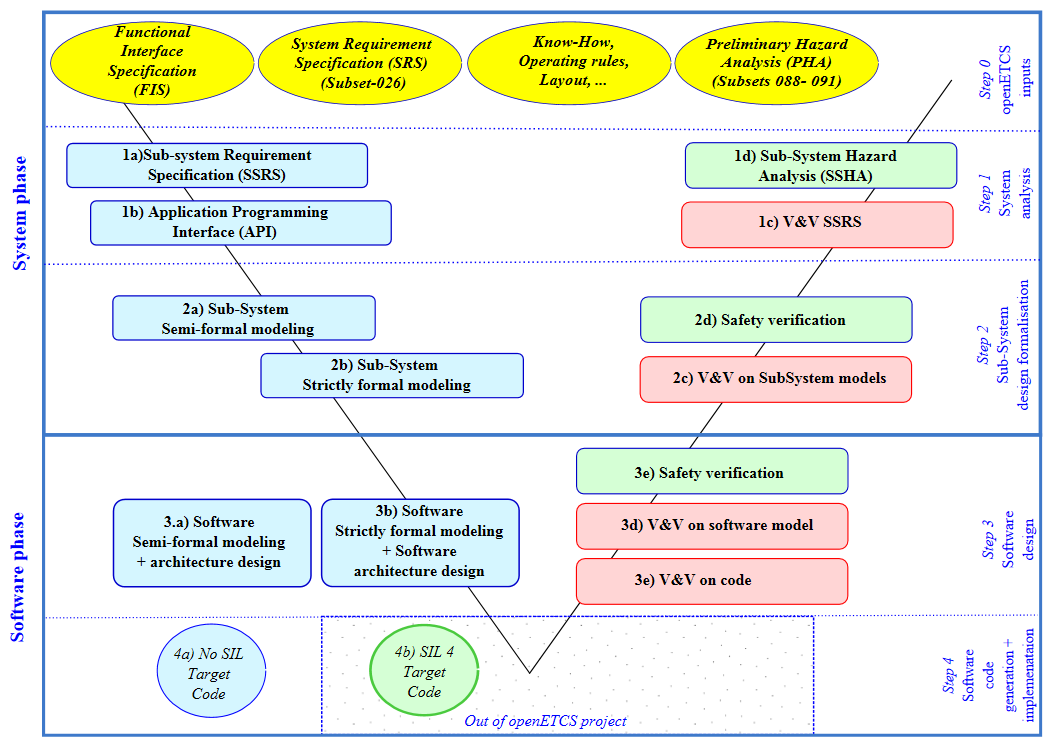
\includegraphics[width=.9\textwidth]{images/ProcessOpenETCS-BeM.png}
%   \caption{openETCS Process (rough view)}
%   \label{fig:openETCSProcess}
% \end{figure}
% %
% As a basis for planning the V\&V activities, the process sketch
% permits to name the main phases. Planning will need a
% better definition of the stages (scope of the design artifacts,
% level of detail, respective system boundaries), detailed planning a
% specification of the artifacts to be produced. Version V01 of this
% document will in these respects be of an accordingly preliminary
% nature. 
 

\part{\VV for a Full Development }



\nthng{
W.r.t.\ \vv, openETCS shall achieve two goals:
\begin{enumerate}
\item Design a tool-supported method with which the EVC software can
  be developed and maintained so that it is suitable for integration
  in (SIL-4) certified products. This will be described in
  Sec.~\ref{sec:vv-strategy-full}, ``\VV Strategy for a Full Development''.
\item Perform part of the development (including tool and method
  evaluation and the study of tool qualification questions) on
  representative parts of the design. The plans for that will be
  detailed in Sec.~\ref{sec:vv-strategy-project}, ``\VV Strategy for openETCS''.
\end{enumerate}}

\nthng{
In more detail, the verification and validation have to consider the
following aspects throughout the development process.
%
\begin{itemize}
\item functionalities of the system and the sub-system,
\item system and sub-system architecture,
\item external and internal interfaces of the sub-system,
\item software components,
\item performance and Safety objectives and constraints,
\item functional properties,
\item safety properties.
\end{itemize}}

\chapter{\VV in the openETCS Process}
\label{sec:vv-openETCS-process}

%\input{WP41-V03-Full-Process.tex}

\chapter{\VV Strategy for a Full Development }
\label{sec:vv-strategy-full}

%% \chapter{\VV Strategy for a Full Development }
% \label{sec:vv-strategy-full}



The overall strategy is to support the design process as specified in
D2.3 and its partial instantiations within openETCS. In accordance
with the project approach, V\&V shall be done in a FLOSS style, and it
has to suit a model-based development. A further main consideration
shall be to strive for conformance with the requirements of the
standards (EN~50128 and further). Of particular importance in that
respect is of course the interface to the safety considerations and
the contribution of V\&V to the safety case.

Here, the ideal shall be described: How will the V\&V part of a FLOSS
development of the open-source EVC software look like, what are its
constituents, and how do they act together in developing and
maintaining this software within the openETCS ecosystem.

\section{Verification Strategy for a Full Development}
\label{sec:verif-strategy-full}

This section defines the strategy for verifying a full development of
the EVC software from the requirements source
(ss~026+TSIs+\ldots). This ends with the verification of the
software/hardware integration. In current view, the API defines the
interface and relevant properties of the hardware. Thus, SW/HW
integration for openETCS will most probably done virtually with an
instantiation of the API playing the role of the hardware. 

\subsection{System Test Campaigns}
Testing is one of the main means for verification. The three main
features of test campaigns which need to be specified are:
\begin{itemize}
\item Definition of the different campaigns for each design phase and
  their characteristics.
\item Definition of the campaign objectives, and of the kind of test
  to be performed in order to achieve these objectives.
\item Traceability matrix between characteristics to check/ validate
  and test cases.
\end{itemize}

\subsection{V\&V Actions Criteria}
These criteria shall define the acceptance of system or component
modification, and the interruption criteria shall define the condition
under which a test campaign should be stopped for instance. These
criteria have to bet set during the V\&V plan redaction.  During the
verification phase, these items are verified thanks to the actions
criteria list described in the subpart related to the development
phases and items verification.

\subsection{Organization Charts and Responsibilities} 
The plan shall define the roles and responsibilities of people
involved in the V\&V activities (according to standards and project
needs). Must also be defined the teams compositions, and the
deliverables product owners, as well as the group and committee for
modification.  These items are verified during the verification phase.

\subsection{Internal Means and Tools} 
The plan shall list and define the means and tools needed for V\&V
actions (also when they are needed).  These items are verified during
the verification phase.

\subsection{External Means and Tools} 
The plan shall list and define the means and the tools used by the
interfaces with the project, and which company or structure is using
them.  These items are verified during the verification phase.

\subsection{Development Phases and Item Verification}
\bgcmmnt{Needs to be revised. }

The plan for the development phases verification is based on
requiement coverage at system and sub-system level.  The requirements
are usually decomposed and gathered in a table, and this table
constitutes a road-map for verification activities, and is closely
followed in order to figure out if the required items are covered, and
if so, in which document.  The following items give an overview of
items checked during verification phases, regarding the kind of
prescriptions checked, and the appropriate related development phase.

\begin{description}
\item[Introduction:] This part gives an overview of Verification
  general purposes, of main verification phases (Safety Specification
  of Software, architecture, and overall test campaign), and
  verification support formalism (harmonized against different
  Verification activities, can be a simple table).
\item[ Software Security/Safety Prescriptions Specification Phase:]
  Gives a list of prescriptions (specifications top level from a top
  level specification providing the customer needs), and trace their
  coverage (justification and in which document this justification is
  provided).  Here is an example: ``Prescription specification related
  to Software safety should come out from upper level system safety
  prescriptions and from prescriptions from Security schedule.  This
  information should be communicated to the Software developer.''
\item[Design Phases and Software Development:] This phase is based on
  the same approach of the previous part, and prescriptions are
  gathered in a table.  The different categories considered are
  defined in the following parts: (), , detailed design and
  development prescriptions, coding prescriptions, Software modular
  tests and Software integration tests prescriptions.
\item[General Requiements:] For instance: design representations shall
  be based on a clearly defined notations, or limited to clearly
  stated characteristics
\item[Software Architecture Related Requirements:]. For instance: Any
  System Safety prescription modification related to security should
  be documented and acknowledged by the developer.
\item[Support Tools and Coding Languages Requirements:]. For instance:
  According to the type of development, the compliance with the given
  prescriptions is under the software supplier responsibility.
\item[Detailed Design and Development Prescriptions:] For instance:
  ``The Software shall be produced in order to insure the required
  modularity, testability and modification ease.''
\item[Coding Prescriptions:] For instance: ``Each Software code
  module shall be reviewed''
\item[Software Modular Tests Prescriptions:] For instance: ``Modular
  tests shall be documented''
\item[Software Integration Tests Requirements:] For instance:
  ``Integration test specification shall encompass: integration groups
  easily manageable, test cases and test data, test kinds,
  environment, tools configuration on test program, test acceptance
  criteria, corrective actions procedures''
\item[Software Security Validation Planning:] The same formalism as
  previous parts can be used, and this part sums up the different
  requirements/specification for the planning regarding the safety
  activity. For instance: ``Planning shall be managed in order to
  specify technical and process steps necessary to prove that the
  software is compliant with safety prescriptions''.
\item[Programmed Electronic Components (Hardware and Software):] This
  part is specifically related to the integration conditions. This
  part is not supposed to be considered in openETCS, as no
  integration is planned in the project so far.
\item[Software Safety Validation:] For instance: ``Validation
  activities shall be performed as specified in the validation plan''.
\item[Conclusion:] (related to the requirements coverage). In our
  case, the prescriptions are the requirements explained in the WP4
  (these prescriptions have to be refined from the different project
  inputs, such as CENELEC, SRS, FPP\ldots).
\end{description}


\section{Validation Strategy for a Full Development}
\label{sec:valid-strategy-full}

Validation, according to the standard, starts after SW/HW
integration. In this section, it shall be detailed how this should
look like for the openETCS architecture approach (with SSRS and
API). Ideal would be a description of how a full openETCS EVC software
could be taken up by some manufacturer and brought to life in a
product (validation aspect only, of course). Validation will use tests
covering operational scenarios.  

Not-so-classical validation can start earlier when executable models
become available. If a model can be animated to run an operational
scenario (perhaps with some additional environment/rest-of-system
modeling), design defects may get unveiled before the real
validation. This is, however, not an activity which is mentioned as a
development activity in the standard EN~50128. Thus, to use results of
``early validation'' in a validation report requires a definition of
its role and an argument for its usefulness.

\subsection{Validation Case}
The aim of the Validation Report is to demonstrate that the objectives
of validation which have been set in the validation plan have been
achieved. This concerns the adequacy of the software design
documentation and that components and system behavior is compliant
with the software requirements.

The inputs for validation at system level are:
\begin{itemize}
\item Software Requirement Specification (design, architecture),
\item Sub-System Requirement Specification (encompassing the architecture, 
interface description and requirement allocation),
\item Application Programming Interface,
\item Internal and External constraints,
\item Validation constraints list,
\item Validation Plan,
\end{itemize}

The inputs for validation at software level are:
\begin{itemize}
\item Components Requirements Specification,
\item Integration Specification,
\item Integration Report,
\item Test Specifications,
\item Test reports.
\end{itemize}


The outputs are:
\begin{itemize}
\item Software Validation Report (Verdict on software ability to fulfill 
the objectives and functionalities defined in the requirement specification.),
\item Software Validation Verification Report,
\end{itemize}

\section{Safety Interface}
\label{sec:safety-interface}

\bgcmmnt{There are two aspects: (1) Safety requirements come from a hazard
and risk analysis. (2) The main contribution of \vv of the openETCS SW
of the EVC for the safety case of the
EVC (HW and SW) should be the validation report of the software. This
has to prove that the software as implement achieves all its safety
goals which have been assigned to it. These two aspects are adressed
(partly) in D4.2.3. The following text should be adapted.}

The safety activities in the software development process are closely
connected to the \vv activities as these provide the overall system
safety requirements, derive corresponding safety related design
specifications and collect the \vv documentation to build the safety
case. The safety activities are identifying unwanted accidents
resulting in harm and analyses the potential hazards, which could lead
to the harm. Resulting from this in depth analysis certain
requirements are derived, which provide the overall safety goals for
the system. If the initial risk of a hazard resulting in harm has to
be reduced or the possibility of harm shall be eliminated at all
specific safety designs are developed to reach the required risk. The
\vv process has to verify these specifications and validated that the
requirements hold for the developed software. Respectively, a complete
documentation is needed to show in the safety case that this steps
have been done according to the overall \vv plan.

Therefore three main interfaces to the safety activities have to be
maintained in the \vv process:
\begin{itemize}
\item \textbf{Verification of safety design specification}: Based on
  risk control measures documented in the Hazard Log specific safety
  design specifications are derived and written in the backlogs for
  model and code development. As it is done for the overall model and
  code specification the verification activities have to demonstrate
  that all of the safety specifications have been implemented
  properly.
\item \textbf{Validation of safety requirements}: The overall software
  validation has to demonstrated that the safety goals are met by the
  developed product. Therefore the safety requirements which have been
  stated based on potential accidents and accepted risk levels have to
  be validated. As these in many cases requires proof for the absence
  of certain conditions, it is important that \vv activities work in a
  close iterations with the safety activities to ensure that the
  safety requirements are stated in a way that can be validated.
\item \textbf{Creation of \vv documentation}: As the safe case has to
  provide the complete argumentation that all needed steps to ensure a
  qualified and safe development process have been performed properly,
  it is important that the \vv plan and all resulting \vv reports are
  coherent and allow to show a close chain of arguments.
\end{itemize}




\chapter{Verification Plan for a Full Development}
\label{sec:verification-plan-full}

%% \chapter{Verification Plan for a Full Development}
% \label{sec:verification-plan-full}

\nthng{
\texttt{Contributors to this chapter:
  \begin{description}
  \item[DLR] Overall coherence, revise structure of the Verification Report
  \item[All4Tec] Role of model-based testing, \qq{hopefully more}
  \item[SQS] Overall coherence
  \item[CEA] Tools and methods Sec.~\ref{sec:methods-tools})
  \item[U Bremen] Tools and methods (model based testing, bounded
    model checking Sec.~\ref{sec:methods-tools}),
    V\&V process steps
  \item[Fraunhofer] Tools and methods Sec.~\ref{sec:methods-tools})
  \item[TUBS] Safety Interface, general tool list
  \item[TWT, URO] Tools and methods Sec.~\ref{sec:methods-tools})
  \item[DB, SNCF, NS] operator role (end user scenarios, validation
    requirements and contribution)
  \item[Institut Telecom] Methods and Tools Sec.~\ref{sec:methods-tools})
  \end{description}
}
}

The section is going to instantiate the generic \VV plan from the standard to
the EVC development in openETCS-style (FLOSS). This entails the organisation,
a definition of the requirements, 
generic schedule covering all design steps, resources, responsibilities, 
tools, techniques, and methodologies to be 
deployed in order to perform the verification activities, and all the
documents which are to be produced.

The result must conform to the requirements of the standards for a
SIL~4 development.

  As D2.3 gives only a rough description of the development steps and
  not yet a complete list of design artifacts, nor one of methods
  applied and formats to be used, this first version (V01) of the V\&V plan
  will also lack detail which will to be added in later revisions as
  these informations become more concrete.

\section{\VV Plan Overview}
\label{sec:plan-overview}

This section gives an overview of the \vv plan for a full development. 

\subsection{\VV Organisation}
\label{sec:vv-organisation}

This section defines the relationship of verification and validation
to other efforts such as development, project management, quality
assurance, and configuration management. It defines the lines of
communication within the \vv, the authority for resolving issues, and
the authority for approving \vv deliverables. Here, the \vv aspect of
the ``openETCS-ecosystem'' should be outlined.



\subsection{\VV Activity Overview}
\label{sec:vv-activity-overview}

This section gives a short overview of the activities (Verification or
Validation) which happen at the respective development steps, to be
detailed in the subsequent sections. The numbering (e.g.\ 2e) refers
to Fig.~\ref{fig:openETCSProcess}. Abbreviations used are defined in
the glossary, Sec.~\ref{sec:glossary}.

\begin{description}
\item[SSRS---Verification (1c):] verification that the SSRS the requirements
  consistently extends the requirements base. 
\item[SSRS---Validation (1c):] Deriving a sub-system test specification
\item[SFM---Verification (2c):] Verification that the model formalises
  the requirements
\item[SFM---Validation (2c):] Detailing the test specification,
  perhaps validating the model (e.g.\ via animation)
\item[SW-SFM---Verification (3d):] Verifying the SW-HW architecture
  definition (should be somewhere) and the software model
\item[SW-SFM---Validation (3d):]Perhaps validation of the software model
\item[SW-FFM---Verification (3d):]  verification, employing also
  formal methods/tools 
\item[SW-FFM---Validation (3d):] validation, may e.g.\ employ model checkers
\item[Code---Verification (3e):] verification depends on the code
  generation method (manual, generated, generated with validated
  tool), unit test requirements have to be met, afterwards code
  integration tests
\item[Code---Validation (3e):] no specific activities foreseen
\end{description}

The following step descriptions are preliminary and shall serve as a
concept which is to be detailed in later revisions (V02 and up).
%
\begin{description}
\item[EVC Software---Verification (tbd):] Perform software system verification
\item[EVC Software---Validation (tbd):] Validation against user
  requirements/scenarios, broken down to software functionality
\item[SW/HW integration (tbd):] Use the API in a simulation
  environment as a replacement of actual SW/HW integration
\item[Final Validation (tbd):] Apply user (railway operator) requirements and scenarios (based
  on the sub-system test specification)
\end{description}

\subsection{Schedule}
The overview of the activities given above shalle be detailed in this
section. The objective here is to define an orderly flow of material
between project activities and verification tasks.  

\nthng{It describes the project life cycle and project milestones
  including completion dates.  Summarize the schedule of verification
  tasks and how verification results provide feedback to the whole
  openETCS process to support overall project management functions.
  The objective of this section is to define an orderly flow of
  material between project activities and verification tasks.}

\subsection{\VV Resources}
\label{sec:vv-resources}

In a regular development project, resources needed to perform
verification tasks, including staffing, facilities, tools, finances,
and special procedural requirements such as security, access rights,
and documentation control, have to be defined. Here, where we define
merely a pattern of a V\&V plan, the emphasis will lie on spelling out
requirements and proposing
principal solutions.
\nthng{  
\textit{Guidance: This section summarizes the resources needed to
  perform verification tasks, including staffing, facilities, tools,
  finances, and special procedural requirements such as security,
  access rights, and documentation control.}
}

\subsection{Responsibilities}
\label{sec:vv-responsibilities}

\nthng{
\textit{Guidance: Identify the organization responsible for performing Verification tasks. There are two levels of responsibility--- 
general responsibilities and specific responsibilities for the verification tasks to be performed should be assigned to individuals. Here, in the general \vv plan, only the first are to be defined.}
}
\begin{center}
\begin{longtable}{|m{2,5cm}|m{6cm}|m{2cm}|m{2cm}|}
\caption{General \VV Responsibilities}
\label{tab:gener-vv-respo}\\

\hline \rowcolor{myblue} \multicolumn{1}{|c|}{Role} &
\multicolumn{1}{|c|}{Name of the person} &
\multicolumn{1}{|c|}{Affiliation} & \multicolumn{1}{|c|}{Activity
  Code} \\ \hline
\endfirsthead

\multicolumn{4}{c}%
{{\bfseries \tablename\ \thetable{} -- continued from previous page}} \\
\rowcolor{myblue} \multicolumn{1}{|c|}{Role} &
\multicolumn{1}{|c|}{Name of the person} &
\multicolumn{1}{|c|}{Company} & \multicolumn{1}{|c|}{Activity Code} \\
\hline
\endhead

\hline \multicolumn{4}{|r|}{{Continued on next page}} \\ \hline
\endfoot

\hline \hline
\endlastfoot

Verification Team Manager & & & \\\hline
Verifier & & & \\\hline
\end{longtable}
\end{center}

\section{Requirements Base}
\label{sec:requirements-base}

This section shall provide references to all requirements 
against which the design is to be verified and validated. It does not include 
process requirements. For the latter, see Sec.~\ref{sec:appendix}.

The requirements on the EVC software origin in the SS-026 and TSI
specifications.




\section{Verification Acitivities for a Full Development}
\label{sec:verif-full-devel}

\textit{for each of the verification steps identified in the plan
  overview, the following has to be instantiated: }
\subsection{DAS2V Verification}
\label{sec:dasv-verification}

\subsubsection{Task}
\label{sec:dasv-verif-task}

\subsubsection{Documents to Be Produced}
\label{sec:dasv-verif-docum-be-prod}

\subsubsection{Phase Specific Activities}
\label{sec:dasv-verif-phase-spec-activ}

\subsubsection{Techniques and Measures}
\label{sec:dasv-verif-techniques-measures}

\textit{Here the verification plan begins}

\subsection{SSRS Verification (1c)}
\label{sec:ssrs-verification}

\subsubsection{Task}
\label{sec:ssrs-verif-task}

The SSRS (sub-system requiement specification) outlines the subsystem
which is going to be modeled within the project. The SSRS describes
the architecture of the subsystem (functions and their I/O) and the
requirements allocated to these functions. If necessary, the
requirements are rewritten in order to address the I/O and to
correspond to the allocation. It also provides the classification into
vital and non vital requirements and data
streams. The architecture part is described in a semi-formal language,
and the requirements are described in natural language.

The SSRS is to be viewed as a supplement to the SS-026 and the
TSIs and is not intended to replace them. The verification has to
check that a complete and consistent set of functionalities have been
identified and that the architecture is adequate. 

%\todo{Verifiy hazard analysis too?}


\subsubsection{Documents to Be Produced}
\label{sec:ssrs-verif-docum-be-prod}

SSRS verification report.

\subsubsection{Phase Specific Activities}
\label{sec:ssrs-verif-phase-spec-activ}

\subsubsection{Techniques and Measures}
\label{sec:ssrs-verif-techniques-measures}

 Due to the informal
nature of the SSRS, mainly manual techniques are to be applied.

\qq{Review}



\subsection{SFM Verification (2c)}
\label{sec:sfm-verif-verification}

\subsubsection{Task}
\label{sec:sfm-verif-task}

\subsubsection{Documents to Be Produced}
\label{sec:sfm-verif-docum-be-prod}

\subsubsection{Phase Specific Activities}
\label{sec:sfm-verif-phase-spec-activ}

\subsubsection{Techniques and Measures}
\label{sec:sfm-verif-techniques-measures}




%\todo{further verification phases}

\subsection{System Verification}
%\textcolor{red}{<Brief Introduction>}

\paragraph{SSRS Verification(1c)}
The SSRS Verification phase refers to the task already defined in the
Sec.~\ref{sec:ssrs-verification} of this document that involves the
full development.  For further details about the activities involved,
please go to the mentioned section.

\subsubsection{Software Verification}
\label{sec:sw-verif}

This section describes software verification activities in greater
detail than the description above. This presentation of the material
shall be unified in due course.

The SW process is detailed in the D.2.3 OpenETCS process. Bearing in
mind that the tasks described in this openETCS Verification plan are
strongly linked to the Software process defined in that document, the
following figure is included in order to have present the key points
to be covered in the plan.

\begin{figure}[h]
  \centering
  \fbox{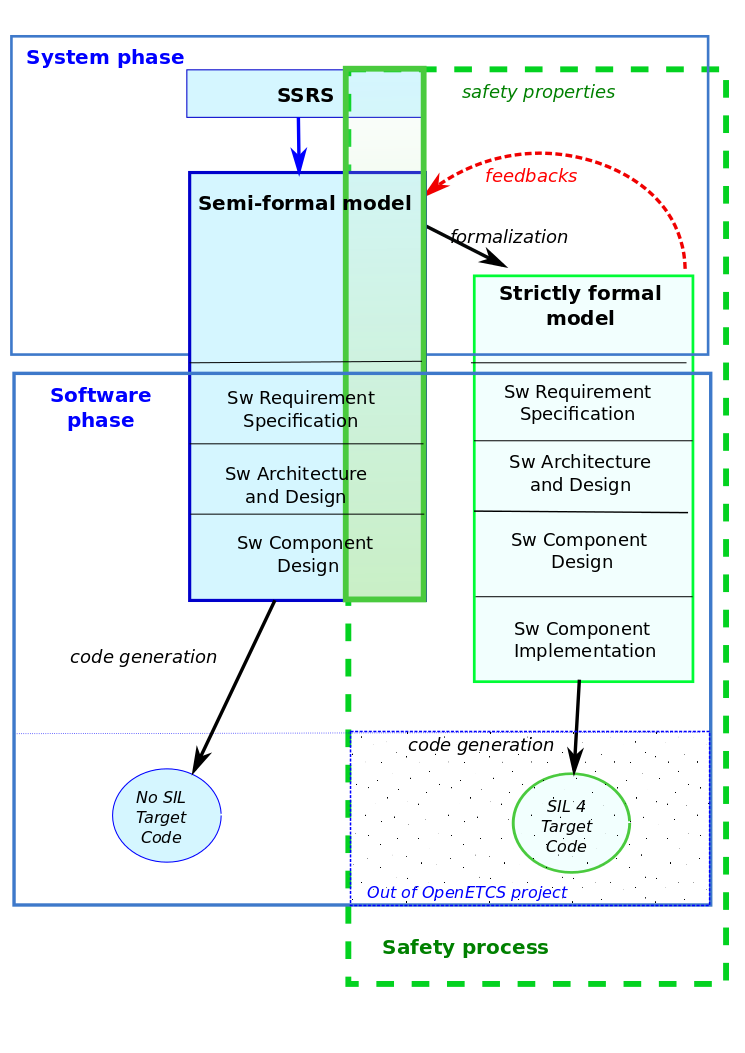
\includegraphics[width=4in]{Model-phase.png}}
  \caption{Software phase description}
  \label{fig:detailed software}
\end{figure}

\textbf{SW Requirements Verification}

\underline{Task} 

In the SW Requirements Specification the SSRS shall be taken as
starting point, redefining it to ensure the software constraints are
considered.  The SW Requirements Verification phase then shall verify
that the proposed Software Requirements cover as much as possible of
the SSRS and provide a correct implementation of the System
Requirements in the Software context.  On the other hand, the
Verification done in this phase shall include the assessment of the SW
Requirements modelling, the objective is to ensure the representation
of the requirements is coherent with their specification as well as
complete, explicit and implementable, as well as traceable to the
semi-formal and/or formal models defined in the system phase.

\underline{Documents to Be Produced} 

\begin{itemize}
\item SW Requirements Verification Report
\end{itemize}

\underline{Activities}

Some activities shall be performed to ensure the requirements are
written in a readable and testable manner. The Verification of the
Software Requirements shall assess whether the requirements met the
following aspects:
\begin{itemize}
\item Deterministic: Given an initial system state and a set of
  inputs, you must be able to predict exactly what the outputs will
  be.
\item Unambiguous: All openETCS project members must get the same
  meaning from the requirements; otherwise they are ambiguous.
\item Correct: The relationships between causes and effects are
  described correctly.
\item Complete: All requirements are included. There are no omissions.
\item Non-redundant: Just as the Software modelling (semi-formal and
  formal) provides a non-redundant set of data, the requirements
  should provide a non-redundant set of functions and events.
\item Lends itself to change control: Requirements, like all other
  deliverables of the openETCS project, should be placed under change
  control.
\item Traceable: SW Requirements must be traceable to each other, to
  the SSRS, to the objectives, to the design, to the test cases, and
  to the code.
\item Readable by all project team members: The project stakeholders,
  including the users, experts and testers, must each arrive at the
  same understanding of the requirements.
\item Written in a consistent style: Requirements should be written in
  a consistent style to make them easier to understand.
\item Explicit: Requirements must never be implied.
\item Logically consistent: There should be no logic errors in the
  relationships between causes and effects.
\item Lends itself to reusability: Good requirements can be reused on
  future projects based on openETCS.
\item Succinct: Requirements should be written in a brief manner, with
  as few words as possible.
\item Annotated for criticality: Each SW requirement should note the
  level of criticality to the openETCS project. In this way, the
  priority of each requirement can be determined, and the proper
  amount of emphasis placed on developing and testing each
  requirement.
\item Feasible: If the software design is not capable of delivering
  the requirements, then the requirements are not feasible.
\end{itemize}

The activities that shall ensure these aspects are successfully met
are the following:
\begin{itemize}
\item {\it SWReq-Ver-Act1. Compliance with SSRS}: the SW Requirements
  are based on the SSRS, so it shall be ensured that their
  specification is compliant and coherent with regard to the SSRS; the
  SW requirements complement, adjust and enlarge the scope delimited
  by the SSRS in the Software phase.
\item {\it SWReq-Ver-Act2. Accuracy, Consistency, Completeness,
    Correctness assurance}: A significant problem with recording
  requirements as text is the difficulty of analyzing them for
  completeness, consistency, and correctness. The Specification of the
  SW Requirements has precise syntactic and semantic rules (e.g., data
  type consistency) and the specification of the requirements shall be
  compared against those established rules to ensure these aspects are
  correctly covered.
\item {\it SWReq-Ver-Act3. Testability assurance}: The two objectives
  for testing the openETCS safety-critical SW are the demonstration
  that the software satisfies its requirements and the demonstration
  that errors that could lead to unacceptable failures have been
  removed.
\item {\it SWReq-Ver-Act4. Verificability assurance}: The SW
  Requirements shall identify the main functionality and describe the
  functional breakdown and data flows from top-level functions to
  low-level functions. The description provided as well as the flows
  identified shall be verifiable.
\item {\it SWReq-Ver-Act5. Compliance with Standards}: Compliance with
  CENELEC Standards (EN50126, EN50128 and EN50129) shall be verified.
\item {\it SWReq-Ver-Act6. Traceability with SSRS}: Each SSRS
  allocated to software must map to one or more software
  requirement. Traceability analysis, which can be automated,
  determines the completeness of the mapping of SSRS to software. A
  table similar to this one shall be obtained, either manually or
  automatically to assess the conformance with this expected activity.
\item {\it SWReq-Ver-Act7. Requirements modelling correctness}:
  Considering "the result of the modelling activities is a document
  that represents a thorough understanding of the problem the proposed
  software is intended to solve"\textcolor{red}{[1. Cho, Chin-Kuei,
    Quality Programming, John Wiley \& Sons, Inc, 1987, p 21.]},
  during the SW Requirements verification, it shall be possible to
  capture all required information, including additional information
  for safety-critical aspects with the support of the models. These
  Requirements representations shall be compared to their original
  specification and assess whether they are complete and enough to
  cover all the information provided by them.
\end{itemize}

\begin{center}
\begin{longtable}{|m{5cm}|m{7cm}|}
  \caption{Requirements Trace Table}\\
  \hline \rowcolor{myblue} \multicolumn{1}{|c|}{Source SSRS ID} &
  \multicolumn{1}{|c|}{SW Requirement ID} \\ \hline
\endfirsthead
\multicolumn{2}{c}%
{{\bfseries \tablename\ \thetable{} -- continued from previouqs page}} \\
\rowcolor{myblue} \multicolumn{1}{|c|}{Source SSRS ID} &
\multicolumn{1}{|c|}{SW Requirement ID} \\ \hline
\endhead
\hline \multicolumn{2}{|r|}{{Continued on next page}} \\ \hline
\endfoot
\hline \hline
\endlastfoot
SSRS-xxxx &
SWR-yyy
\\\hline
SSRS-xxxx &
SWR-yyy
\\\hline
\end{longtable}
\end{center}

\underline{Tools, Techniques, Methods and Measures} 

This section shall identify the special software tools, techniques, and
  methodologies to be employed by the verification team. 
The purpose of each should be defined and plans for the acquisition,
training, support, and qualification of each shall be described in
this section.

The following table summarizes the Techniques, methods, measures or
tools proposed for the identified activities. 

\begin{center}
\begin{longtable}{|m{1,5cm}|m{8,5cm}|m{4cm}|}
  \caption{SW Requirements Verification Tools, Techniques, Methods and Measures}\\
  \hline \rowcolor{myblue} \multicolumn{1}{|c|}{Activity} &
  \multicolumn{1}{|c|}{Techniques/ Methods/ Measures} &
  \multicolumn{1}{|c|}{Tools}\\ \hline
\endfirsthead
\multicolumn{3}{c}%
{{\bfseries \tablename\ \thetable{} -- continued from previous page}} \\
\rowcolor{myblue} \multicolumn{1}{|c|}{Activity} &
\multicolumn{1}{|c|}{Techniques/ Methods/ Measures} &
\multicolumn{1}{|c|}{Tools} \\\hline
\endhead
\hline \multicolumn{3}{|r|}{{Continued on next page}} \\ \hline
\endfoot
\hline \hline
\endlastfoot
{\it SWReq-Ver-Act1} & 
This compliance is verified by peer review. The first version of SW
Requirements is usually incomplete and composed primarily of top-level
adjustments. The meaning of the SW requirements is described
textually. & 
<To be defined>  
\\\hline
{\it SWReq-Ver-Act2} & 
Since the modelling at this stage is provided, verification is mostly
based on review and with a tools-based modelling approach. Some
consistency checks between the SW Requirements and both the
semi-formal modelling and the formal modelling can be automated. 
& 
<To be defined>  
\\\hline
{\it SWReq-Ver-Act3} &
Requirements-based testing has been found to be effective at revealing
errors early in the testing process Requirement models created with
standard UML use-case notations are not robust enough to create
requirements based test cases that met the safety-critical aspects, so
the standard use-case model notation shall be extended to allow the
capture of additional information required to determine test cases. & 
Test cases can be automatically generated from ``test-ready'' use-case
models. <To be defined>   
\\\hline
{\it SWReq-Ver-Act4} & 
Verification is mostly based on review &
<To be defined> 
\\\hline
{\it SWReq-Ver-Act5} & 
Verification is mostly based on review &
<To be defined>
\\\hline
{\it SWReq-Ver-Act6} & 
A traceability matrix between SSRS and SW Requirements shall be
prepared either manually or automatically and assessed by review &  
Integrated tools can generate software to system requirements
traceability tables showing which software requirements are allocated
to system requirements. <To be defined> 
\\\hline
{\it SWReq-Ver-Act7} & 
Verification is mostly based on review & 
<To be defined>
\\\hline
\end{longtable}
\end{center}

\textbf{SW Architecture, Design and Modelling Verification}

\underline{Task} 

This phase aims to ensure that the software architecture design
adequately fulfils the software requirements specification already
verified in the SW Requirements Verification phase. 
The software architecture defines the major elements and subsystems of
the openETCS software, how they are interconnected, and how the
required (safety integrity) attributes will be achieved. It also
defines the overall behaviour of the software, and how the software
elements interact.  
To carry this phase the information from the current software
lifecycle phase shall be verified. All essential information should be
available and must be verified; the information should include the
adequacy of the specifications, design and plans in the current phase.  
The architecture and design shall be modelled and the coherence of
those models with regard to their specification shall be verified to
assess whether the constraints are correctly treated. 
The verification configuration should be precisely defined and the
verification activities shall be repeatable. 

\underline{Documents to Be Produced} 

\begin{itemize}
\item SW Architecture, Design and Modelling Verification Report
\end{itemize}

\underline{Activities}

Software architecture verification should consider whether the
software architecture design adequately fulfils the SW requirements
specification.  

The essential properties to be verified during this phase are:

\begin{itemize}
\item What is the software supposed to do: including the SW
  specification and the system capabilities
\item What is the software not supposed to do: be aware of the
  unexpected emergent behaviour, boundary specifications, inhibits
\item What is the software supposed to do under adverse conditions:
  system biases, tolerances
\item What are the safety considerations
\item What are the integration or interfacing considerations:
  subsystems, modules, components, relationship between hardware and
  software, partitions, parallelism, compatibility 
\item What are the dependability considerations: performance,
  capacity, complexity, stability
\end{itemize}

Considering these aspects, a table shall be prepared to list a
relation of verification dimensions regarding to the Architecture and
Design that facilitates the process. An example is given below:

\begin{center}
\begin{longtable}{|m{2cm}|m{2cm}|m{2,1cm}|m{2cm}|m{1cm}|m{2cm}|m{2,1cm}|}
\caption{SW Architecture Verification preparation table - Example of contents}\\
\hline \rowcolor{myblue} \centering \textbf{Verification dimension} &
\centering \textbf{Intended behaviour} & \centering
\textbf{Unacceptable behaviour} & \centering \textbf{Adverse
  conditions} & \centering \textbf{Safety} & \centering
\textbf{Integration} & \textbf{Dependability} \\\hline  
\endfirsthead
\multicolumn{7}{c}%
{{\bfseries \tablename\ \thetable{} -- continued from previous page}} \\
\rowcolor{myblue} \centering \textbf{Verification dimension} &
\centering \textbf{Intended behaviour} & \centering
\textbf{Unacceptable behaviour} & \centering \textbf{Adverse
  conditions} & \centering \textbf{Safety} & \centering
\textbf{Integration} & \textbf{Dependability} \\\hline  
\endhead
\hline \multicolumn{7}{|r|}{{Continued on next page}} \\ \hline
\endfoot
\hline \hline
\endlastfoot
Performance analysis & Service delivery & Consequences of service
failure, unexpected emergent behaviour & Distributed redundancy and
fail-over & & &   
\\\hline
Timing Requirements & normal behaviour & Blown performance margins,
missing timing requirements & Distributed redundancy and fail-over &
Safety and Recoverability, timing margins & Timeline  
management, phase transition interlocks &   
\\\hline
Security Requirements & Secure communication & Compromised
communication & Redundant communication channels & & &  
\end{longtable}
\end{center}
The software architecture modelling, which consists of determining and
connecting software components, requires a phase of analysis to be
able to validate the representation carried out, as errors can occur
in the representation. It is thus necessary to be able to identify and
to provide them to the designer.  

Modelling must also bring answers in term of feasibility and the
constraint shall be analyzed so the interdependent functions should
not overlap.

The verifications done at the software architecture level are related
to specification and execution model coherency.

The expected activities for this phase are the following:
\begin{itemize}
\item {\it SWArch-Ver-Act1. Check the software architecture design}:
  The SW architecture and design should fulfil the SW requirements
  specification. From a safety point of view, the software
  architecture phase is where the basic safety strategy for the
  software is developed. 
\item {\it SWArch-Ver-Act2. Handle attributes}: The attributes of
  major elements and subsystems should be adequate with reference to
  the feasibility of the safety performance required, testability for
  further verification, readability by the development and
  verification team, and safe modification to permit further
  evolution. With the attributes, on which we rely once the software
  is specified, it is possible to check if the model of execution and
  the coherence of the periods of the various software components are
  corrects. 
\item {\it SWArch-Ver-Act3. Check incompatibilities}: The
  incompatibilities between design and specification should be
  checked.  
\item {\it SWArch-Ver-Act4. Model coherency}: Verify the
  representation carried out with the modelling. The errors identified
  can be related to the symmetry of the inter-connected functions. A
  certain number of constraints of coherence must thus be analyzed.  
\item {\it SWArch-Ver-Act5. Constraints analysis}: Ensure system
  dysfunctions do not occur. Some components can also execute an
  operation depending on a signal resulting from another component,
  which results in constraints of synchronization that must also be
  taken into account.  

\end{itemize}

\underline{Tools, Techniques, Methods and Measures} 

The specific software tools, techniques, and methodologies to be
employed by the verification team are to be identified here.  The
purpose of each should be defined and plans for the acquisition,
training, support, and qualification of each shall be described in
this section.

The following table summarizes the Techniques, methods, measures or
tools proposed for the identified activities.

\begin{center}
\begin{longtable}{|m{1,5cm}|m{8,5cm}|m{4cm}|}
\caption{SW Architecture, Design and Modelling Verification Tools,
  Techniques, Methods and Measures}\\ 
\hline \rowcolor{myblue} \multicolumn{1}{|c|}{Activity} &
\multicolumn{1}{|c|}{Techniques/ Methods/ Measures} &
\multicolumn{1}{|c|}{Tools}
\\ \hline 
\endfirsthead
\multicolumn{3}{c}%
{{\bfseries \tablename\ \thetable{} -- continued from previous page}} \\
\rowcolor{myblue} \multicolumn{1}{|c|}{Activity} &
\multicolumn{1}{|c|}{Techniques/ Methods/ Measures} &
\multicolumn{1}{|c|}{Tools} 
\\\hline
\endhead
\hline \multicolumn{3}{|r|}{{Continued on next page}} \\ \hline
\endfoot
\hline \hline
\endlastfoot
{\it SWArch-Ver-Act1} & 
 & 
<To be defined> 
\\\hline
{\it SWArch-Ver-Act2} & 
&  
<To be defined> 
\\\hline
{\it SWArch-Ver-Act3} &
&
<To be defined> 
\\\hline
{\it SWArch-Ver-Act4} & 
 &
<To be defined> 
\\\hline
{\it SWArch-Ver-Act5} & 
 &
<To be defined> 
\\\hline
\end{longtable}
\end{center}

\textbf{SW Component and Modelling Verification}

\underline{Task} 

This phase analyzes whether the SW components defined in the openETCS
Software process are verifiable by design, with a focus on the formal
verification of data aspects of components and components modelling.
This task requires a detailed understanding not only of the
corresponding specification, but also the environments and methodology
in which the verification component will be used.

This phase delivers methods and tools to

\begin{itemize}
\item Verify the component models by model-checking techniques, with a
  focus on behavioural aspects such as attributes and data-dependent
  properties 
\item Verify the specification of the components is coherent to the SW
  architecture and design previously verified. This activity shall be
  based on the existing models in the component stage as well as
  previous phases, in close connection with the model checking
  activities. 
\end{itemize}

\underline{Documents to Be Produced} 

\begin{itemize}
\item SW Component and Modelling Verification Report
\end{itemize}

\underline{Activities}

This phase aims to assess whether the specification and modelling of
components are reusable, configurable, and implementable in the
expected code automatically generated environment.

\begin{itemize}
\item Within the context of the models that contain the components
  identified for the SW phase, the verification of components within a
  control system model shall be required.  As standalone components ---
  For a high level of confidence in the component algorithm, verify
  the component in isolation from the rest of the components and
  sub-systems identified. This approach is called component analysis.
\item Verifying standalone components provides several advantages:
\begin{itemize}
\item The analysis can be be used to focus on portions of the design
  that cannot be tested because of the physical limitations of the
  system being controlled.
\item This approach can be used for open-loop simulations to test the
  plant model without feedback control.
\end{itemize}
\end{itemize}

The components shall be identified at the points of minimal coupling
(minimal control and/or information exchange) and decompose the
specification. The smaller components might be amenable to be verified
and how to abstract these parts of the specification shall be
analysed.

The rest of the specification could be exposed to formal analysis,
such as model checking or theorem proving. The abstraction reduces the
number of states that need to be checked by an automated verification
technique and helps in avoiding the state explosion problem, which
occurs in traditional model checking.

An approach to specification decomposition is slicing the system
specifications represented with Petri Nets. In this way, the
specification shall improve the understanding of the complexity of the
system and high-risk components can be identified earlier.

The activities that shall ensure these aspects are successfully met
are the following:
\begin{itemize}
\item {\it SWComp-Ver-Act1. Verify components with minimal coupling
    independently of the model}: Within this activity a component
  analysis shall be performed to verify model blocks, atomic
  subsystems and statechart atomic subcharts. After extracting the
  blocks, or contents of the subsystems and subcharts, a harness model
  shall be created for the referenced model and the extracted model
  with the contents of the subsystem o subchart. A Test suite shall be
  prepared and executed to record coverage and output values. The Code
  Generation Verification (CGV) shall be invoked to execute the test
  cases on the generated code for the model that contains the
  component.
\item {\it SWComp-Ver-Act2. Verify components with minimal coupling in
    the context of the model}: A similar process shall be conducted in
  this case but performing a system analysis to verify the model
  blocks in the context of the model.
\item {\it SWComp-Ver-Act3. Formal analysis of components}: Perform
  model checking of components against properties; the results
  obtained shall highlight that: the component satisfies the
  properties for the environment; the component violates the
  properties for the environment; characterization of those
  environments in which the components satisfied each property.
\end{itemize}

Regarding the Modeling Verification, the activities involved shall ensure that:
\begin{itemize}
\item The models have been designed correctly and covers all the parts
  involved in the openETCS project
\item The algorithms have been implemented properly
\item The models do not contain errors, oversights, or bugs
\item The specification is complete and that mistakes have not been
  made in implementing the model
\end{itemize}

Each of the models defined in the full development context shall be
developed for a specific purpose and its validity is determined with
respect to that purpose. It shall be considered that a model that may
be valid for one set of conditions, can be invalid in another; because
of that, the model's output variables of interest shall be clearly
identified and their required amount of accuracy be specified.

It is costly and time consuming to determine whether a model is valid
over the complete domain of the full development context. Instead,
tests and evaluations are conducted until sufficient confidence and
certainty is obtained that a model can be considered valid. In the
model verification activities, tests are performed, errors are
identified, and corrections are made to the underlying models while
the models are exercised for the identified cases. Furthermore, the
verification of the models can result in retesting requirements to
ensure code integrity.

If the verification process determines that a model does not have
sufficient accuracy for any one of the sets of identified conditions,
then the model is invalid. However, determining that a model has
sufficient accuracy for numerous conditions does not guarantee that a
model is valid everywhere in its applicable domain.

\begin{itemize}
\item {\it SWModel-Ver-Act1.} 
\item {\it SWModel-Ver-Act2. }  
\item {\it SWModel-Ver-Act3. }
\end{itemize}

\underline{Tools, Techniques, Methods and Measures} 

The specific software tools, techniques, and methodologies to be
employed by the verification team are to be identified here. 
The purpose of each should be defined and plans for the acquisition,
training, support, and qualification of each shall be described in
this section. 

The following table summarizes the Techniques, methods, measures or
tools proposed for the identified activities.

\begin{center}
\begin{longtable}{|m{1,5cm}|m{8,5cm}|m{4cm}|}
\caption{SW Component and Modelling Verification Tools, Techniques,
  Methods and Measures}
\\
\hline \rowcolor{myblue} \multicolumn{1}{|c|}{Activity} &
\multicolumn{1}{|c|}{Techniques/ Methods/ Measures} &
\multicolumn{1}{|c|}{Tools}\\ \hline  
\endfirsthead
\multicolumn{3}{c}%
{{\bfseries \tablename\ \thetable{} -- continued from previous page}} \\
\rowcolor{myblue} \multicolumn{1}{|c|}{Activity} &
\multicolumn{1}{|c|}{Techniques/ Methods/ Measures} &
\multicolumn{1}{|c|}{Tools} \\\hline 
\endhead
\hline \multicolumn{3}{|r|}{{Continued on next page}} \\ \hline
\endfoot
\hline \hline
\endlastfoot
{\it SWComp-Ver-Act1} & 
 & 
<To be defined>  
\\\hline
{\it SWComp-Ver-Act2} & 
& 
<To be defined>  
\\\hline
{\it SWComp-Ver-Act3} &
 &
 <To be defined>  
\\\hline
{\it SWModel-Ver-Act1} & 
 &
<To be defined> 
\\\hline
{\it SWModel-Ver-Act2} & 
 &
<To be defined>
\\\hline
{\it SWModel-Ver-Act3} & 
 & 
<To be defined>
\\\hline

\end{longtable}
\end{center}

\textbf{SW code generation Verification}

\underline{Task} 

This phase analyzes whether the generated code from the model is
correct, robust, complete, coherent and reliable, with a focus on the
formal verification and on the equivalence of the model and the
generated code.

This phase delivers methods and tools to

\begin{itemize}
\item Verify the equivalence between the model and the generated code
  by equivalence testing and dynamic testing techniques
\item Verify the correctness of the translation algorithm and its implementation
\item Verify the complexity, coding guidelines and syntax of the
  generated code by static analysis techniques
\item Verify the robustness of the generated code
\end{itemize}

\underline{Documents to Be Produced} 

\begin{itemize}
\item SW Code Generation Verification Report
\end{itemize}

\underline{Activities}

When in the other phase the confidence in the correctness of the model
has been verified, it is necessary to have high confidence in the
generated code.

To achieve verified code generation, it is not sufficient to only
verify the code generation algorithm due to the implementation of the
algorithm might introduce errors as well. It is necessary to
distinguish between the correctness of the translation algorithm
itself and the correctness of its implementation.

Within the context of the Code Generation Verification, the code
generation verification approach shall utilize translation testing to
demonstrate that the execution semantics of the model are preserved
during production code generation, compilation and linking

The validity of the translation process, i.e. whether or not the
semantics of the model have been preserved during code generation,
compilation and linking, shall be determined by comparing the system
reactions

The activities that shall ensure these aspects are successfully met
are the following:
\begin{itemize}
\item {\it SWCode-Ver-Act1. Semantic Properties Verification}: For
  safety reasons, it is necessary that the generated code is
  semantically equivalent to the original model specification to
  ensure correct software and system behavior.

  During this activity, the semantics of the original model is
  preserved during the code generation shall be demostrated. This will
  verify that the transformation algorithm is correct.

\begin{figure}[h]
  \centering
  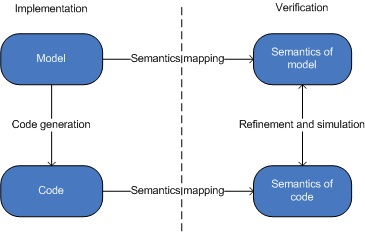
\includegraphics[scale=1]{images/transformation_verification.jpg}
  \caption{Transformation Verification}
  \label{fig:transformationver}
\end{figure}

To prove the semantical correctness of such a transformation, a
suitable model semantics is needed.

As a basic prerequisite, the semantics of the model and code must be
comparable and it is also required a semantics for both model and code
with the same semantic domain.

The first steps will be define the commom both model and code
semantics. A multitude of approaches can be taken to define such a
semantics. This definintion of the semantics poses subtle difficulties
due to inherent ambiguities. Once this is done the coverage over
semantics shall be identified.

Then, it will be necessary to establish a correspondence between the
model and code, based on refinement, and to prove it by simulation.

A refinement mapping correlating the control points of the model and
code, and indicating how the relevant model variables correspond to
the code variables or expressions at each control point shall be
established. For some transformation optimizations it is often
impossible to apply the refinement based rule since there are often no
control points where the states of the model and code can be
compared. So, a large class of these optimizations shall be identified
to allow their effective transformation verification.

After this, the simulation method shall be used for transformation verification. 

This transformation from model to code will be considered semantically
correct if the semantics of model and code are always the same.

Using the simulation principle to show that are equal, a simulation
relation in which they are contained shall be found and defined. Note
that the definition of a simulation relation is an artificial
construct for conducting proofs.


\item {\it SWCode-Ver-Act2.  Functional Correctness Verification}:
  Within this activity, as a first approach for functional properties
  correctness verification, the automatic test cases generated from
  the model will be executed under the automatic generated code from
  the same model, so that, the coherence, functionality and coverage
  of the code shall be verified.

  Taking into account the first obtained results, it will be possible
  to check the coverage of both code and test cases, detect the
  necessary functional properties not generated automatically, and
  they shall be inserted manually into the code.

  When discrepances are found, an analysis of both test cases and code
  shall be done to check in which part the problem is taking into
  account the techniques and tools of the specific verification phase
  activities.


\item {\it SWCode-Ver-Act3. Quality Properties (Complexity, Syntax,
    coding guidelines) Verification}: Within this activity, a static
  analysis shall be performed locating potentially vulnerable code.

  The static analysis involves no dynamic execution and will detect
  possible faults such as unreachable code, undeclared variables,
  parameter type mismatches, uncalled functions and procedures,
  possible array bound violations, standards fulfillment i.e. MISRA
  standard, etc.

The static analysis techniques will also include:
\begin{itemize}
\item \underline{data flow analysis}: it consists in a technique to
  follow the path that various specific items of data take through the
  code, looking for possible anomalies in the way the code handles the
  data items
\item \underline{control flow analysis}: technique for determining the
  control flow of the code. This type of analysis will identify
  infinite loops, unreachable code, cyclomatic complexity that
  identifies the number of decision points in a control flow, other
  complexity metrics like number of nested statements, etc.
\end{itemize}

With this analysis, errors in the structure and syntax of the code are
going to be found but run-time errors (errors that only occur when the
code is executed) will not be detected as we are not running the code.

Therefore this will not find things like memory leaks or check whether
a value in a variable is correct.

\item {\it SWCode-Ver-Act4. Equivalence Verification}: This activity
  shall use equivalence testing and other techniques like dynamic
  testing to demonstrate equivalence between the model and the
  generated code.
 
  During this phase, the execution of the model used for code
  generation and the object code derived from it with the same input
  stimuli followed by a comparison of the outputs shall be
  performed. The validity of the translation process, i.e. whether or
  not the semantics of the model have been preserved during code
  generation, compilation and linking, is determined by comparing the
  system reactions (results, which are the outputs resulting from
  stimulation with identical timed test inputs) of the model and the
  generated code.

  If the coverage achieved with the existing test inputs is not
  sufficient w.r.t. the selected model coverage metrics, additional
  test inputs that execute the model elements not covered shall be
  created. In practice, the tester can iteratively extend the set of
  test inputs using model coverage analysis until the chosen level of
  model coverage has been achieved. If full coverage for the selected
  metric(s) cannot be achieved, the uncovered parts shall be assessed
  and justification for uncovered parts shall be provided.
\item {\it SWCode-Ver-Act5. Robustness Verification}: Within this
  activity a code analysis shall be performed to verify its robustness
  so it behaves reasonably in exceptional situations; wrong execution
  paths, computational errors or erroneous inputs and memory
  alterations coming from the environment(errors caused by
  interactions between the software and its environment(hardware and
  software))

  The exceptional situations coming from the software itself can be
  automatically proven using static analyzers based on abstract
  interpretation such as Frama-C or RSM

  After this analysis, there will be necessary to check the
  exceptional situations coming from the environment. The
  inconsistencies between the specification and the user constrains
  present in the code shall be detected. To ensure the robustness of a
  piece of code, the value of each un-trusted input must be checked
  against its correctness domain after its production and before its
  consumption

  The robustness review of the generated code can be done by manual
  code review to verify that all checks are present at right locations
  and that the checked domains are strictly included in the
  correctness domains.
\end{itemize}

\underline{Tools, Techniques, Methods and Measures} 

The specific software tools, techniques, and methodologies to be
employed by the verification team are to be identified here. 
The purpose of each should be defined and plans for the acquisition,
training, support, and qualification of each shall be described in
this section. 

The following table summarizes the Techniques, methods, measures or
tools proposed for the identified activities.

\begin{center}
\begin{longtable}{|m{3cm}|m{7cm}|m{4cm}|}
\caption{SW Code Generation Verification Tools, Techniques, Methods
  and Measures}\\ 
\hline \rowcolor{myblue} \multicolumn{1}{|c|}{Activity} &
\multicolumn{1}{|c|}{Techniques/ Methods/ Measures} &
\multicolumn{1}{|c|}{Tools}\\ \hline  
\endfirsthead
\multicolumn{3}{c}%
{{\bfseries \tablename\ \thetable{} -- continued from previous page}} \\
\rowcolor{myblue} \multicolumn{1}{|c|}{Activity} &
\multicolumn{1}{|c|}{Techniques/ Methods/ Measures} &
\multicolumn{1}{|c|}{Tools} \\\hline 
\endhead
\hline \multicolumn{3}{|r|}{{Continued on next page}} \\ \hline
\endfoot
\hline \hline
\endlastfoot
{\it SWCode-Ver-Act1} & 
 & 
<To be defined>  
\\\hline
{\it SWCode-Ver-Act2} & 
& 
<To be defined>  
\\\hline
{\it SWCode-Ver-Act3} &
 &
 <To be defined>  
\\\hline
{\it SWCode-Ver-Act4} & 
 &
<To be defined> 
\\\hline
{\it SWCode-Ver-Act5} & 
 &
<To be defined>
\\\hline

\end{longtable}
\end{center}

\textbf{Traceability matrix Verification}

\underline{Task} 

The Traceability Matrix is a resource to ensure that the project's
scope, requirements, modeling and generated code remain as are
expected to be when compared to the objectives to be reached. The
matrix traces the different elements by establishing a thread for each
requirement to the corresponding model and component, the generated
code that consists on its implementations and the test cases defined.

\begin{itemize}
\item The specifications shall be verified following the traces
  between the elements defined in the matrix
\item With the matrix verification it shall be ensured that all the
  required information is included in the specification, such as
  process models and data models
\item Requirements that are not addressed by configuration items
  during design and code reviews can be identified; in a similar way,
  extra configuration items that are not required can be highlighted
\item The verification of the matrix shall provide input to change
  requests and future project plans when missing elements are
  identified
\end{itemize}

\underline{Documents to Be Produced} 

\begin{itemize}
\item Traceability Matrix Verification Report
\end{itemize}

\underline{Activities}

Taking the time to cross-reference each element involved in the
project to another element ensures that the results obtained by each
phase of the project are consistent with the requirements, the
modeling and the code.

To accomplish this objective it shall be verified that the
traceability matrix is in the following format:

\begin{itemize}

\item The matrix generated is a two-dimensional table,
\item There is one column per identified element (such as requirement,
model, components, or code),
\item A check mark at the end of the table shall be put if all the row
is well traced, coherent and unambiguous
\item Various traceability matrices may be utilized throughout the
project life cycle.  \item At least the matrices shall contain the
following elements:
\begin{itemize}
\item Formal specification of Requirements: It shows that each
requirement (obtained from SSRS) has been covered in an appropriate
section of the formal specification.
\item Design specification through modeling to functional
specification, this verifies that each function has been covered in
the design.
\item System test plan to functional specification ensures the test
case or test scenario for each process, component and each requirement
in the functional specification have been identified
\end{itemize}
\end{itemize}

\underline{Tools, Techniques, Methods and Measures}

The specific software tools, techniques, and methodologies to be
employed by the verification team are to be identified here.  The
purpose of each should be defined and plans for the acquisition,
training, support, and qualification of each shall be described in
this section.

The following table summarizes the Techniques, methods, measures or
tools proposed for the identified activities.

\begin{center}
\begin{longtable}{|m{1,5cm}|m{8,5cm}|m{4cm}|}
\caption{Traceability Matrix Verification Tools, Techniques, Methods
  and Measures}\\ 
\hline \rowcolor{myblue} \multicolumn{1}{|c|}{Activity} &
\multicolumn{1}{|c|}{Techniques/ Methods/ Measures} &
\multicolumn{1}{|c|}{Tools}\\ \hline  
\endfirsthead
\multicolumn{3}{c}%
{{\bfseries \tablename\ \thetable{} -- continued from previous page}} \\
\rowcolor{myblue} \multicolumn{1}{|c|}{Activity} &
\multicolumn{1}{|c|}{Techniques/ Methods/ Measures} &
\multicolumn{1}{|c|}{Tools} \\\hline 
\endhead
\hline \multicolumn{3}{|r|}{{Continued on next page}} \\ \hline
\endfoot
\hline \hline
\endlastfoot
{\it SWMatrix-Ver-Act1} & 
 & 
<To be defined>  
\\\hline
{\it SWMatrix-Ver-Act2} & 
& 
<To be defined>  
\\\hline
{\it SWMatrix-Ver-Act3} &
 &
 <To be defined>  
\\\hline

\end{longtable}
\end{center}

\textbf{Test Verification}

\underline{Task} 

Verification of the test suites designed for testing, the conformance
of the implementation of the specifications, the design, the models
and/or the code generated against the formal description of the
openETCS system shall involve the verification of some relevant
aspects of the test cases such as:

\begin{itemize}
\item expected input/output of the test behaviour
\item test results
\item test purpose
\end{itemize}

The properties of the test cases shall be defined as they were
liveness properties, providing notations to specify the test purpose
formally. All these properties expressed with formal notation can be
verified using model checking, for example, on an extended state
machine diagram, so the behaviour of the test case is
represented. With this methodology, errors in the specification of the
test cases can be found easily.

\underline{Documents to Be Produced} 

\begin{itemize}
\item Test Verification Report
\end{itemize}

\underline{Activities}

There are two approaches when designing a test suite:
\begin{itemize}
\item \textit{Semi-automatic generation of test-cases}: the formal
  specification of the system is used to generate the test
  cases. Previously there has been identified some test design
  techniques that generate test cases. However there could be some
  features, like the robustness capabilities of implementation, that
  cannot be derived to test cases using semi-automatic techniques.
\item \textit{Human design of test cases}: human designed test suites
  have some advantages over the semi-automatic ones that shall be
  taken into account, for example that the test case can be designed
  with a specific test purpose, the test cases can be grouped into
  various categories (basic interconnection tests, capability tests,
  valid behaviour tests, robustness/invalid behaviour tests, etc.) and
  the test cases can be manually designed for complex
  architectures. On the other hand these test cases, due to they have
  been designed manually, can be error-prone.
\end{itemize}

The test suites designed during the openETCS project shall combine
both strategies, so in general terms some of them shall be generated
semi-automatically following different techniques to be reviewed and
adjusted later by the test engineers to ensure their appropriateness,
and for the most specific contexts, the required experience and
knowledge shall involve a manual design and a methodology to verify
the correctness of those test cases against the formal specification.

Considering these aspects when designing the test suites, the
following activities shall be done to verify the correctness and
completeness of the tests cases generated:

\begin{itemize}
\item {\it SWTest-Ver-Act1. Verification of semi-automatic generated
    test cases}: The verification of the test case shall imply to
  check whether the essential information has been correctly
  generated. For example: are sufficient input combinations
  exercised?, are the tests complete and enough to find defects?, the
  conditions have been collected in the test cases, the test cases
  test one specific thing each to simplify the tracking of errors and
  obtain high coverage, the test cases say how the system works, the
  test cases are correctly organised in test suites and they keep the
  consistency so it will be easy to locate and add new test cases in
  the future, and finally assess whether the test cases are:
\begin{itemize}
\item Fast: The test cases shall be fast to execute, the running
  should not take much time.
\item Independent: The test cases can be run in any order. 
\item Repeatable: The result of the test case should be always the
  same, no matter how many times it has been executed.
\item Small: Small test cases are easy to understand and change, are
  also likely to be faster.
\item Transparent: It should be clear what the purpose of each test case is.
\end{itemize} 
\item {\it SWTest-Ver-Act2. Verification of manual designed test
    cases}: the verification process is similar to the process already
  defined in the verification of semi-automatic generated test cases
  activity. Besides this, some aspects related to the manual
  specification of test cases shall be taken into account like the
  peer-review done to find typical human errors, robustness and
  completeness checking or general coherence.
\end{itemize}


\underline{Tools, Techniques, Methods and Measures} 

The specific software tools, techniques, and methodologies to be
employed by the verification team are to be identified here. 
The purpose of each should be defined and plans for the acquisition,
training, support, and qualification of each shall be described in
this section. 

The following table summarizes the Techniques, methods, measures or
tools proposed for the identified activities.

\begin{center}
\begin{longtable}{|m{1,5cm}|m{8,5cm}|m{4cm}|}
\caption{Test Verification Tools, Techniques, Methods and Measures}\\
\hline \rowcolor{myblue} \multicolumn{1}{|c|}{Activity} &
\multicolumn{1}{|c|}{Techniques/ Methods/ Measures} &
\multicolumn{1}{|c|}{Tools}\\ \hline  
\endfirsthead
\multicolumn{3}{c}%
{{\bfseries \tablename\ \thetable{} -- continued from previous page}} \\
\rowcolor{myblue} \multicolumn{1}{|c|}{Activity} &
\multicolumn{1}{|c|}{Techniques/ Methods/ Measures} &
\multicolumn{1}{|c|}{Tools} \\\hline 
\endhead
\hline \multicolumn{3}{|r|}{{Continued on next page}} \\ \hline
\endfoot
\hline \hline
\endlastfoot
{\it SWTest-Ver-Act1} & 
 & 
<To be defined>  
\\\hline
{\it SWTest-Ver-Act2} & 
& 
<To be defined>  
\\\hline
{\it SWTest-Ver-Act3} &
 &
 <To be defined>  
\\\hline

\end{longtable}
\end{center}

\textbf{Coverage Verification}

\textcolor{red}{(futher development: requirements, model and code
  coverage description in task and activities)}

\underline{Task} 

Test coverage is a measure of test effectiveness and it aims to reach
a sufficient fault removal with contained testing effort. Considering
higher levels of coverage are associated with better quality, this
aspect raises an important practical question of how hard it may be to
increase coverage.

The test coverage shall be influenced by:

\begin{itemize}
\item Modeling complexity
\item Code Complexity
\item Type of functionality
\item Testing team experience in the area to be covered
\end{itemize}

All these factors were related to the level of coverage and quality,
with coverage having an effect even after these
adjustments. Furthermore, the test effort increases exponentially with
test coverage, but the reduction in field problems increases linearly
with test coverage. This suggests that for most cases the optimal
levels of coverage are likely to be well short of 100\%.  The level of
coverage needed shall be analysed in each phase of the project and
adjusted when more information and details are obtained.

\underline{Documents to Be Produced} 

\begin{itemize}
\item Coverage Verification Report
\end{itemize}

\underline{Activities}

One of the key tasks to take into account in the preparation of the
V\&V plan is that the correctness of openETCS system shall be verified
with respect to its specification, while is is also assessed how
complete the specification is and whether it really covers all the
expected behaviours.  Doing an exhaustive verification process is a
great challenge considering we are speaking in terms of
simulation-based verification, where test suites shall be prepared
with finite subsets of input sequences.

In this context, it is essential to measure the exhaustiveness of the
test suite with the support of numerous coverage metrics that reflect
different aspects of the appropriateness of the test suite
designed. The activities to be done to measure the coverage shall be
focused not only on state-based coverage, but simulation-based
verification to the formal verification setting as well.

Then, coverage metrics are used in order to monitor progress of the
verification process, estimate whether more input sequences are
needed, and direct simulation towards unexplored areas of the design
and modeling. The metrics proposed shall measure the part of the
design that has been activated by the input sequences.

The basic approach to coverage in testing, which is recording which
parts of the design were exercised during the execution, cannot be
used in formal verification because formal methods are exhaustive, and
this shall be taken into account when designing the coverage strategy
and dealing with formal methods.

The activities that shall ensure these aspects are successfully met
are the following:

\begin{itemize}
\item {\it SWCover-Ver-Act1. Coverage in model checking}: Important
  advantages of model based testing are formal test specifications
  that are close to requirements, traceability of these requirements
  to test cases, and the automation of test case design. In model
  checking, coverage is a standard measure in testing, but is
  considerable difficult to compute in the context of formal
  verification. With this activity the correctness of the system shall
  be verified with respect to the desired behaviour by checking
  whether the involved models satisfy the formal specifications. The
  correctness and exhaustiveness of the specifications made shall have
  direct influence in the exhaustiveness of the model checking; the
  coverage metrics are the way to check this exhaustiveness and
  address the verification process to unexplored areas of the
  design. One technique to be applied in the activity shall be to
  measure coverage checking whether each output is fully determined by
  the specification, given a combination of input values. There are
  other possibilities, like do a model check for each of the mutant
  designs, and although a way to simplify the process is to use
  non-deterministic variables for mutations, this technique is still
  time consuming and costly, so it can be proposed for the most
  critical scenarios.  The following sub-activities shall be included.
\begin{itemize}
\item {\it SWCover-Ver-Act1.1. Coverage of the properties defined:}
  Model Checking is a method for deciding whether a given design
  satisfies a given formal property: in case the design violates the
  property, the Model Checker provides a trace that demonstrates how
  the property can be violated. On the other hand, when the answer to
  the Model Checking query is positive, most tools terminate with no
  further feedback. However, there can be situations where the
  properties are not as complete as expected and here the skills of
  the verification engineer are essential. For this reason, a sanity
  check for the completeness of the set of properties is to measure
  the coverage of them.
\item {\it SWCover-Ver-Act1.2. Code-based coverage metrics}: This
  activity shall imply the execution of syntactic coverage that shall
  be supported with the syntactic representation of the design with
  respect to which the coverage is measured. It covers the measures
  identified to assess the degree to which the source code obtained by
  automatic generation from the models is tested by particular test
  suites. \\ 
  Among others, the number of code lines executed during the
  simulation shall be measured (statement coverage), as well as the
  functions executed (function coverage), whether all the branches
  defined in each control structure present in the code (branch
  coverage) are executed at least once, the points of entry and exit
  are invoked at least once (decision coverage), the boolean
  sub-expressions (condition coverage), or combination of some of them
  like condition/decision coverage where both decision and condition
  coverage are checked to assess whether both have been satisfied in
  the generated code.
\item {\it SWCover-Ver-Act1.3. State-based model coverage}: It
  measures all the states that have been reached and checked. It is
  the essential measure to take in formal verification. The approach
  proposed is to combine coverage criteria, to use model
  transformations for testing, and to combine state machines with the
  other test models in order to reach a whole overview of the
  correctness and effectiveness of the models and whether these
  specifications are close to requirements.
\item {\it SWCover-Ver-Act1.4. Semantic coverage}: Semantic coverage
  metrics measure the part of the functionality of the design
  exercised by the set of input sequences. In this context, the effect
  of the mutations shall be checked mainly on the satisfaction of the
  specification. The influence of mutations and omissions shall be
  checked on the result of model checking of the specifications, in
  such a way that the influence of omission or the changes of values
  of output variables shall be assessed on the satisfaction of the
  specification in the design. \\Besides this, in path coverage the
  influence of omitting or mutating a finite path on the satisfaction
  of the specification in the design shall be assessed. Within this
  task, all possible mutations can be introduced consistently on each
  occurrence of the mutated element, on exactly one occurrence, or on
  a subset of occurrences, thus resulting in structure, node, or tree
  coverage, respectively. The application of mutations shall be done,
  as said before, in the most critical elements of the design.
\end{itemize}
\item {\it SWCover-Ver-Act2. Functional Test Coverage}: It refers to
  metrics that create reports on the measurement of functionality
  exercised in the design and models obtained. In this area the
  metrics proposed are the control-flow coverage that indicates how
  completely the logical flow of the functional model is traversed,
  and the data path coverage, that indicates how completely the data
  paths have been exercised over a specified set of observable
  values. A list of assertions referring to the variables of the
  design shall be obtained, describing those assertions the conditions
  that may be satisfied during the execution or a state of the
  design. These kind of coverage metrics shall measure what assertions
  are covered by a given set of input sequences.
\item {\it SWCover-Ver-Act3. Simulation-based verification}: Each of
  the metrics identified for the Simulation-based verification is
  addressed to a specific representation of the design or a specific
  verification goal. This activity shall be conducted taking into
  consideration the syntactic coverage and semantic coverage metrics
  perspective and shall contain the following sub-activities:
\begin{itemize}
\item {\it SWCover-Ver-Act3.1. Syntactic coverage metrics}: Syntactic
  coverage metrics shall assume a specific formalism for the
  description of the design and this kind of metrics shall also
  measure the syntactic part of the design when executing a given
  input sequence. In this context, it shall be considered as a
  precondition to reach a high degree of coverage according to
  syntactic-based metrics before moving to other type of coverage
  metrics to apply when performing Simulation-based
  verification. \\The syntactic coverage metrics, as in the Model
  Checking perspective, shall include the Code coverage; the task
  shall be conducted in a similar way with statement and branch
  coverage as the basis, where the coverage is calculated on the basis
  of when these items (branches or statements) are executed at least
  once during the execution of a sequence. The expression coverage
  shall be also applied to check boolean expressions.
\item {\it SWCover-Ver-Act3.1. Semantic coverage metrics}: Semantic
  coverage metrics require the support of the experts involved in the
  design of the system and are more sophisticated than syntactic
  coverage metrics. Similarly to code coverage, a state or a
  transition shall be covered if it is visited during the execution of
  the input sequence. Limited-path coverage metrics shall be applied
  to check what expected sequences of behaviour are exercised; on the
  other hand, transition coverage shall be done as a special case of
  path coverage, but for paths of length 1. As said before, mutation
  coverage is the metric that inspired some important work on coverage
  in model checking; and it can be applied in the contexts of semantic
  coverage and in this specific case, for simulation-based
  verification. In mutation coverage, a small change or mutation ins
  introduced to the design, and it shall be checked whether the change
  leads to an erroneous behaviour.  The coverage shall be measured in
  terms of the percentage of the mutant designs that fail.  The goal
  here shall be to find a set of input sequences such that for each
  mutant design there exists at least one test that fails on it.
\end{itemize}
\end{itemize}

Low coverage indicates a possible incompleteness in the specification,
which may lead to missed bugs in the non-covered parts of the design,
so the levels of coverage shall be continuously monitored in order to
assure the correct flow of the project.

\underline{Tools, Techniques, Methods and Measures} 

The specific software tools, techniques, and methodologies to be
employed by the verification team are to be identified here. 
The purpose of each should be defined and plans for the acquisition,
training, support, and qualification of each shall be described in
this section. 

The following table summarizes the Techniques, methods, measures or
tools proposed for the identified activities.

\begin{center}
\begin{longtable}{|m{3cm}|m{7cm}|m{4cm}|}
\caption{SW Coverage Verification Tools, Techniques, Methods and Measures}\\
\hline \rowcolor{myblue} \multicolumn{1}{|c|}{Activity} &
\multicolumn{1}{|c|}{Techniques/ Methods/ Measures} &
\multicolumn{1}{|c|}{Tools}\\ \hline  
\endfirsthead
\multicolumn{3}{c}%
{{\bfseries \tablename\ \thetable{} -- continued from previous page}} \\
\rowcolor{myblue} \multicolumn{1}{|c|}{Activity} &
\multicolumn{1}{|c|}{Techniques/ Methods/ Measures} &
\multicolumn{1}{|c|}{Tools} \\\hline 
\endhead
\hline \multicolumn{3}{|r|}{{Continued on next page}} \\ \hline
\endfoot
\hline \hline
\endlastfoot
{\it SWCover-Ver-Act1} & 
 & 
<To be defined>  
\\\hline
{\it SWCover-Ver-Act2} & 
& 
<To be defined>  
\\\hline
{\it SWCover-Ver-Act3} &
 &
 <To be defined>  
\\\hline
{\it SWCover-Ver-Act4} & 
 &
<To be defined> 
\\\hline
{\it SWCover-Ver-Act5} & 
 &
<To be defined>
\\\hline
{\it SWCover-Ver-Act6} & 
 & 
<To be defined>
\\\hline

\end{longtable}
\end{center}

\textbf{Safety Verification}

\subsubsection{Tool chain Verification}

Verification of the identified list of tools that have been collected
in the tool chain.


\section{Verification Reporting}
\label{sec:verif-report}


This section describes how the verification activities have to be
documented.  Verification reporting will occur throughout the software
life cycle.  The content, format, and timing of all verification
reports shall be specified in this section.

The following kinds of reports will be generated during the verification process:
\begin{itemize}
\item \textbf{Anomaly reports:} 
\item \textbf{Phase Summary Verification reports:} 
\item \textbf{Final report:}
\end{itemize}

\subsection{Structure of the Verification Report}
\label{sec:struct-verif-report}

The following sketches the structure of the verification report. It
shall cover the following central topics:
\begin{description}\setlength{\parsep}{0pt}\setlength{\itemsep}{0pt}\setlength{\topsep}{0pt}
%\reqfixed{04}{040}{x}
%\subreqfixed{04}{040}{1}{x}
\item[Header] containing all information to identify, this report, the
  authors, the approbation and reviewing entities.
\item[Executive Summary] giving an overview of the major elements from
  all sections. 
\item[Problem Statement] describing the challenges to be answered by
  \VV as well as the decisions to be taken based on the V\&V results
  as well as how to cope with potentially faulty output. It further
  describes the accreditation scope based on the risk assessment done
  on V\&V-level. 
\item[V\&V Requirements Traceability Matrix] links every V\&V artifact
  back to the requirements to measure e.g. test coverage and to
  directly link V\&V results to the requirements. 
\item[Acceptability Criteria,] describing the criteria for acceptance
  of the artifact into the \VV process e.g. as the direct translation
  of the requirements into metrics to measure success, are used
  e.g.\ for burndown charts within the process. 
\item[Assumptions] that are identified during the design of the
  verification and validation strategy and how these assumptions have
  an impact on the verdict by listing capabilities and limitations. 
\item[Risks and Impacts] that come across the execution of V\&V tasks
  together with the impacts foreseen. 
\item[V\&V Design] states how the V\&V process builds up including
  data preparation, execution and evaluation. 
\item[V\&V Methodologies] giving a step-by-step walkthrough of all
  possible V\&V activities including the assumptions, and
  verdict-relevant limitations and criteria for, e.g.,  model
  verification, model-to-code verification, unit testing, integration
  testing and final validation (according to the standard, this
  involves running the software on the target hardware).  
\item[V\&V Issues] describing unsolved V\&V issues and their impact on
  the affected proof or verdict. 
\item[Peer Reviews] going into details on how the community can take
  part and how official bodies and partners are integrated into the
  development and review process. 
\item[Test Plan Definition] going into the details of testing by
  describing among other things: 

\begin{description} 
\item[Title] as a unique identifier to the test plan.
\item[Description] of the test and the test-item giving information
  about version and revision. 
\item[Features] to be tested and not to be tested in combination are
  listed together with information background.  
\item[Entry Criteria] which have to be met by the EVC before a test
  can be started, e.g. that the EVC has to be in level~3 limited
  supervision with the order to switch to level~2. 
\item[Suspension criteria and resumption requirements] are the central
  key to a smooth automation of the tests covering topics like
  \emph{when exiting this test before step 10, which entry criteria
    does it comply to or which resumption sequence has to be executed
    to continue testing}. 
\item[Walkthrough] covering a step-by-step approach of the test plan.
\item[Environmental requirements] going into the details of what is
  needed concerning the test environment, e.g. tools, adapter, data
  preparation. 
\end{description}

\item[Discrepancy Reports] identifying the defects.
\item[Key Participants] describing the assignment and task for each
  role involved.  

\begin{description}
\item[Accreditation of Participants] describing who was accredited to
  which role during the \VV phase. 
\item[V\&V Participants] listing the partners participating in V\&V activities,
\item[Other participants] including other interest groups such as
  reviewer by affiliate partners\footnote{affiliate partners are
    non-funded companies who signed the project cooperation agreement
    and with it get read access to the repositories starting from
    incubation phase to contribute e.g. by reviewing}. 
\end{description}

\item[Timeline] giving the timeline for the baselines as input to the
  V\&V process and identifying when each artifact should be created. 
\end{description}



An example of a summary table of verification activities performed is
given in Table~\ref{tab:verif-activ-summary}.  Such a table should
enter the verification report.

\begin{center}
\begin{longtable}{|m{2cm}|m{6cm}|m{2cm}|m{2cm}|}
\caption{SW Verification Activities Breakdown}\label{tab:verif-activ-summary}\\

\hline \rowcolor{myblue} \multicolumn{1}{|c|}{Activity Code} &
\multicolumn{1}{|c|}{Activity} & \multicolumn{1}{|c|}{Responsibility}
& \multicolumn{1}{|c|}{Status/Link}\\ \hline
\endfirsthead


\multicolumn{4}{c}%
{{\bfseries \tablename\ \thetable{} -- continued from previous page}} \\
\rowcolor{myblue} \multicolumn{1}{|c|}{Activity Code} &
\multicolumn{1}{|c|}{Activity} & \multicolumn{1}{|c|}{Estimated
  Delivery} & \multicolumn{1}{|c|}{Real Delivery} \\ \hline
\endhead

\hline \multicolumn{4}{|r|}{{Continued on next page}} \\ \hline
\endfoot

\hline \hline
\endlastfoot

\rowcolor{lightgray} \multicolumn{4}{|l|}{Phase 0: SW Requirements
  Verification} 
\\\hline
SWReq-Ver-Act1 & Compliance with SSRS verification & & 
\\\hline
SWReq-Ver-Act2 & Accuracy, Consistency, Completeness, Correctness
assurance & & 
\\\hline
SWReq-Ver-Act3 & Testability assurance & & 
\\\hline 
SWReq-Ver-Act4 & Verificability assurance & & 
\\\hline 
SWReq-Ver-Act5 & Compliance with Standards & & \\\hline 
SWReq-Ver-Act6 & Traceability with SSRS verification & & \\\hline
SWReq-Ver-Act7 & Requirements modelling correctness & & \\\hline
\rowcolor{lightgray} \multicolumn{4}{|l|}{Phase 1: SW Architecture and
  Design Verification} 
\\\hline
SWArch-Ver-Act1 & software architecture design verification & & 
\\\hline
SWArch-Ver-Act2 & Handle attributes verification & & 
\\\hline
SWArch-Ver-Act3 & incompatibilities checking & & 
\\\hline
SWArch-Ver-Act4 & Model coherency verification & & 
\\\hline
SWArch-Ver-Act5 & Constraints analysis verification & & 
\\\hline
SWArch-Ver-Act6 & Traceability verification & & 
\\\hline
SWArch-Ver-Act7 & Compliance with Standards verification & & 
\\\hline
\rowcolor{lightgray} \multicolumn{4}{|l|}{Phase 2: SW Component
  Design} 
\\\hline
 & & & \\\hline
\end{longtable}
\end{center}


Also a summary of the tool verification activities is to be included,
as indicated in Table~\ref{tab:tool-verif-summary}.
\begin{center}
\begin{longtable}{|m{1cm}|m{6,5cm}|m{2cm}|m{2cm}|}
\caption{Tool Chain Verification Summary}
\label{tab:tool-verif-summary}\\

\hline \rowcolor{myblue} \multicolumn{1}{|c|}{Activity Code} &
\multicolumn{1}{|c|}{Activity} & \multicolumn{1}{|c|}{Estimated
  Delivery} & \multicolumn{1}{|c|}{Real Delivery} \\ \hline  
\endfirsthead

\multicolumn{4}{c}%
{{\bfseries \tablename\ \thetable{} -- continued from previous page}} 
\\
\rowcolor{myblue} \multicolumn{1}{|c|}{Activity Code} &
\multicolumn{1}{|c|}{Activity} & \multicolumn{1}{|c|}{Estimated
  Delivery} & \multicolumn{1}{|c|}{Real Delivery} 
\\ \hline
\endhead

\hline \multicolumn{4}{|r|}{{Continued on next page}} \\ \hline
\endfoot

\hline \hline
\endlastfoot

\rowcolor{lightgray} \multicolumn{4}{|l|}{Phase 0: Tool chain
  Requirements} 
\\\hline
 & & & \\\hline
\rowcolor{lightgray} \multicolumn{4}{|l|}{Phase 1:} \\\hline
 & & & \\\hline
\end{longtable}
\end{center}

%The structure of the Verification report is already defined in the
%\ref{sec:struct-verif-report} section of this document 

\section{Administrative Procedures}
This section identifies the existing administrative procedures that
are to be implemented as part of the Verification Plan. 
Verification efforts consist of both management and technical tasks.
Furthermore, it is the task of the SQA team to monitor whether the
procedures as defined in the management plans (\cite{QAplan}, [SCMP],
[Review and Revision processes]) are followed. 

\subsection{Problem Report}
The problem reporting procedure is described within the document
Change/Problem Management Process.

Any problem, failure and error encountered during the review
activities (QA. Verification, Validation, Assessment) planned in the
software development life-cycle, problems reported by users and
customers as well as change requests initiated by any of the system
stakeholders will be reported and managed following the Change/Problem
Management Process detailed in
\href{https://github.com/openETCS/governance/tree/master/Change-Problem%20Process}{[governance]} and through the Change/Problem Management Tool.

\subsubsection{Task Iteration Process}
Any change in the requirements (system, sub-systems, sw or components)
require repeated verification and validation activities. 

Once the change is accepted following the change/problem management
procedure, the phases and items affected by it must be
evaluated. These tests will be redesigned to reflect the change in the
requirement and will be executed again. 

In turn, a new analysis of the Software Integrity Level will involve
the analysis of the activities requirements and documentation
presented by the EN50128 standard and include such activities in the
SVVP if necessary. 

\subsubsection{Deviation Process}
The Quality Manager will be informed in the case of detection of a
deviation regarding Verification Plan. In addition, he/she also be
informed if it is deemed necessary by an amendment to the Plan,
whether or not motivated by a deviation 

The Quality Manager will report such incidents to the Project Managers
and with whom shall act appropriately. All persons listed in the
responsibilities section (Sec.~\ref{sec:vv-responsibilities}) shall be
informed of a change in the Verification Plan

\subsubsection{Control Procedure}
Control procedures are specified in the Configuration Management Plan [SCMP]


Verification has to be done in each of the phases of the
development. This chapter is structured according to the verification
reports to be produced.

\setcounter{section}{-1}
\section{Template for Describing a Verification or Validation Activity}
\label{sec:VnV-template}

\begin{tabular}{|p{3.2cm}|p{11cm}|}
  \hline
  \multicolumn{2}{|c|}{\textbf{General description of the activity}} \\\hline
  \textbf{Verification object} & 
  % <artifact(s) title> (<number>)
  \\\hline
  \textbf{Responsible role} & 
  % VER | VAL
  \\\hline
  \textbf{Reference material} & 
  % Often used
  % standard(s): \cite{EN50128:2011}, \cite{EN50126:1999},
  % Development process: \cite{openETCS:D2.3a-V02}
  % FPP
  \\\hline
  \textbf{Objective} & 
  % one or two sentences describing the general goal of VnV here
  \\\hline
  \textbf{Evidential material} & 
  % e.g. test documentation
  \\\hline
  \textbf{Method(s)} & 
  % e.g. (most often) Review, could be formal proof, tool-supported
  \\\hline
  \textbf{Documentation} & 
  % Text document, specific review sheet, ...
  \\\hline
\end{tabular}


\begin{tabular}{|p{3.2cm}|p{11cm}|}
  \hline
  \multicolumn{2}{|c|}{\textbf{Detailed description of the objective}} \\\hline
  \textbf{Formalities} & 
  % List the formalities to be checked here.
  % Formalities in general concern the unambiguity of references,
  % consistency in terms, formal completeness of requirement capture
  \\\hline
  \textbf{Traceability} & 
  % Describe what is to be established here for the tracing, i.e. that
  % tracing is done adequately here 
  \\\hline
  \textbf{Completeness} & 
  % Define the completeness to be checked here.
  % Completeness check that the content completely covers the
  % requirements, so these requirements are to be described and
  % referenced here
  \\\hline
  \textbf{Correctness} & 
  % Define the correctness checks
  % e.g. correct refinement of requirement items 
  \\\hline
  \textbf{Consistency} & 
  % Define the consistency to be checked
  % e.g. interfaces match, no contradictions in result properties 
  \\\hline
\end{tabular}

%
\begin{tabular}{|p{3.2cm}|p{11cm}|}
  \hline
  \multicolumn{2}{|c|}{\textbf{Detailed description of the
      documentation [Option 1]}} \\\hline
  \textbf{Template}  &
   % Provide a reference to a documentation template, or include the template
  \\\hline
\end{tabular}

%
\begin{tabular}{|p{3.2cm}|p{11cm}|}
  \hline
  \multicolumn{2}{|c|}{\textbf{Detailed description of the
      documentation [Option 2]}} \\\hline
  \textbf{Managerial items} & 
  % Referencing of input and output, contributing persons, dates,
  % If applicable: tool versions, verdict type 
  \\\hline
  \textbf{[Output item/section \textit{nn}]} & 
  % Iterate for the different output parts
  % Include tool qualifications if applicable
  \\\hline
\end{tabular}



\begin{tabular}{|p{3.2cm}|p{11cm}|}
  \hline
  \multicolumn{2}{|c|}{\textbf{Detailed description of the activity}} \\\hline
  \textbf{Activity steps} & 
  % Describe the steps and their contributions (how they fit together) 
  \\\hline
  \textbf{Step \textit{nn}} & 
  % Describe each step: Goal, Input, Output, Means
  \\\hline
\end{tabular}



\section{Verification of Planning}
\label{sec:verification-full-0}

These verifications are done by reviewing the documents. The results
are collected in the Planning Verification Report (0-05).

\subsection{Verification of the Project Plan}
\label{sec:verification-full-00}

% \paragraph{General description of the activity}
% \begin{description}
% \item[Object of verification:] Project Plan (0-00)
% \item[Responsible:] VER
% \item[Reference material:] EN~50126, EN~50128, FPP, openETCS Process (D2.3a)
%   \item[Objective:] Establish that the project plan defines a viable
%     management structure, where all activities are assigned properly
%     and adequately.
%   \item[Evidential material:] --
%   \item[Method:] Review
%   \item[Documentation:] \textit{tbd}
% \end{description}

\begin{tabular}{|p{3.2cm}|p{11cm}|}
  \hline
  \multicolumn{2}{|c|}{\textbf{General description of the activity}} \\\hline
  \textbf{Verification object} & Project Plan (0-00)
  \\\hline
  \textbf{Responsible role} & VER
  \\\hline
  \textbf{Reference material} & EN~50126, EN~50128, FPP, openETCS
  Process (D2.3a)
  \\\hline
  \textbf{Objective} & Establish that the project plan defines a viable
  management structure, where all activities are assigned properly
  and adequately.
  \\\hline
  \textbf{Evidential material} & --
  \\\hline
  \textbf{Method} & Review
  \\\hline
  \textbf{Documentation} & Text document
  \\\hline
\end{tabular}

\begin{tabular}{|p{3.2cm}|p{11cm}|}
  \hline
  \multicolumn{2}{|c|}{\textbf{Detailed description of the objective}} \\\hline
  \textbf{Formalities} & \textit{tbd}
  % List the formalities to be checked here.
  % Formalities in general concern the unambiguity of references,
  % consistency in terms, formal completeness of requirement capture
  \\\hline
  \textbf{Traceability} & --
  % nothing to check, here
  \\\hline
  \textbf{Completeness} & \textit{tbd}
  % Define the completeness to be checked here.
  % Completeness check that the content completely covers the
  % requirements, so these requirements are to be described and
  % referenced here
  \\\hline
  \textbf{Correctness} & \textit{tbd}
  % Define the correctness checks
  % e.g. correct refinement of requirement items 
  \\\hline
  \textbf{Consistency} & \textit{tbd}
  % Define the consistency to be checked
  % e.g. interfaces match, no contradictions in result properties 
  \\\hline
\end{tabular}

%
\begin{tabular}{|p{3.2cm}|p{11cm}|}
  \hline
  \multicolumn{2}{|c|}{\textbf{Detailed description of the
      documentation}} \\\hline
  \textbf{Managerial items} & \textbf{Input:} [Project plan version],
  \textbf{Output:} [Project plan verification report version],
  \textbf{Responsible person:} [person of role VER],
  \textbf{Contributors:} [list], \textbf{Date:} [date]
  \\\hline
  \textbf{[Output item/section \textit{nn}]} & 
  % Iterate for the different output parts
  % Include tool qualifications if applicable
  \\\hline
\end{tabular}



\begin{tabular}{|p{3.2cm}|p{11cm}|}
  \hline
  \multicolumn{2}{|c|}{\textbf{Detailed description of the activity}} \\\hline
  \textbf{Activity steps} & \textit{tbd}
  % Describe the steps and their contributions (how they fit together) 
  \\\hline
  \textbf{Step \textit{nn}} & \textit{tbd}
  % Describe each step: Goal, Input, Output, Means
  \\\hline
\end{tabular}


\subsection{Verification of the Quality Assurance Plan}
\label{sec:verification-full-01}

%\input{WP41-V03-Full-01}

\subsection{Verification of the Configuration Management Plan}
\label{sec:verification-full-02}

%\input{WP41-V03-Full-02}

\subsection{Verification of the Verification Plan}
\label{sec:verification-full-03}

%\input{WP41-V03-Full-03}

\subsection{Verification of the Validation Plan}
\label{sec:verification-full-04}

%\input{WP41-V03-Full-04}

\subsection{Planning Verification Report}
\label{sec:verification-full-05}

Sec.~\ref{sec:verification-full-05} gives an overview of the components of the Planning
Verification Report. Its main parts are described in the 
subsections of Sec.~\ref{sec:verification-full-0} preceding this
subsection (Sec.~\ref{sec:verification-full-05}).
%\input{WP41-V03-Full-05}


\section{Verification of the System Design}
\label{sec:verification-full-1}


\section{Verification of the Sub-System Architecture Design}
\label{sec:verification-full-2}


\subsection{Verification of the Sub-System Architecture Design}
\label{sec:verification-full-13}

%\input{WP41-V03-Full-13}

\subsection{Verification of the Acceptance Plan}
\label{sec:verification-full-14}

%\input{WP41-V03-Full-14}

\subsection{Sub-System Architecture Design Verification Report}
\label{sec:verification-full-15}

%\input{WP41-V03-Full-05}

\section{Verification of the SW Specification}
\label{sec:verification-full-3}


\section{Verification of the SW Design}
\label{sec:verification-full-4}

\section{Verification of the SW Component Implementation and Test}
\label{sec:verification-full-5}

\section{Verification of the SW Integration}
\label{sec:verification-full-6}

\section{Verification of the SW Validation}
\label{sec:verification-full-7}




\chapter{Validation Plan for a Full Development}
\label{sec:validation-plan-full}

%% \chapter{Validation for a Full Development}
% \label{sec:valid-full-devel}


For each of the validation steps identified in the plan
  overview, the following has to be instantiated:

\section{DAS2V Validation}
\label{sec:dasv-validation}

\subsection{Task}
\label{sec:dasv-valid-task}


\subsection{Documents to Be Produced}
\label{sec:dasv-valid-docum-be-prod}


\subsection{Phase Specific Activities}
\label{sec:dasv-valid-phase-spec-activ}

\subsection{Techniques and Measures}
\label{sec:dasv-valid-techniques-measures}



\section{SFM Validation (3d)}
\label{sec:sfm-validation}

\subsection{Task}
\label{sec:sfm-valid-task}

The formalisation of the requirements in form of a semi-formal model
enables a systematic check of the completeness and consistency of the
system test specification.

The model itself can perhaps be animated (depending on the concrete
form which is not yet fixed). This offers the chance to an early
(preliminary) validation of the design.

\subsection{Documents to Be Produced}
\label{sec:sfm-valid-docum-be-prod}

\begin{enumerate}
\item Revised System Test Specification
\item SFM validation report
\end{enumerate}

\subsection{Phase Specific Activities}
\label{sec:sfm-valid-phase-spec-activ}

\tbd{}

\subsection{Techniques and Measures}
\label{sec:sfm-valid-techniques-measures}

\tbd{}

\section{Final Validation (tbd)}
\label{sec:final-validation}

\subsection{Task}
\label{sec:final-valid-task}

The final validation shall ascertain that the end result of the
development---the EVC software in its specified environment---behaves
as required. 

\subsection{Documents to Be Produced}
\label{sec:final-valid-docum-be-prod}

\begin{enumerate}
\item System Test Definition (based on System Test Specification)
\item System Validation Report
\end{enumerate}

\subsection{Phase Specific Activities}
\label{sec:final-valid-phase-spec-activ}

Testing the software against the user requirements.

\subsection{Techniques and Measures}
\label{sec:final-valid-techniques-measures}

A technique to be considered is testing in a validated testbed
(including API animation/simulation).





\part{\VV Plan for the Project openETCS}

\chapter{\VV Strategy for the Project openETCS}
\label{sec:vv-strategy-project}

%
% \chapter{\VV Strategy for the Project openETCS}
% \label{sec:vv-strategy-project}

\paragraph{Scope of \VV in openETCS}

The project will only perform part of the development, and thus also
only a part of the V\&V activities. These need to be defined and
planned. The overall approach shall be to try out the different
constituents on and in representative samples, so that the
realisability of the \vv strategy for a full development can
covincingly be demonstrated.

Besides the usual purpose of \vv activities, namely evaluating and
proving the suitability of design artifacts, V\&V in openETCS will
also generate information on the suitability of the methods and tools
employed. For that purpose, a format for describing methods and tools
to be used in V\&V and one for summarizing the findings about the
suitability are defined.

\paragraph{Implementing SCRUM}
The overall project approach is to organise activities in an agile
way, following the ideas behind the SCRUM development
method. This has two main aspects for V\& V (in the following text,
\emph{verification} is used to also include validation):

\begin{enumerate}
\item \label{SCRUM-Artifacts} Artifacts are produced in iterations and
  expected to be verified iteratively.
\item \label{SCRUM-Split} Verification activities are split over
several iteration, where each should produce some useful result.
\end{enumerate}

Adressing (\ref{SCRUM-Artifacts}), it is recommended to not attempt to
derive a final verdict, except in cases where a set of requirements
are claimed to be covered completely. Preliminary models or code parts
can serve to evaluate tools and methods, and to set up verification
environments, to be able to complete the verification when the
artifact is a more final state. Preliminary artifacts should be
assessed for their aptness for the intended v\&v. Feedback on
deficiencies will help to accelerate later activities.

Concerning (\ref{SCRUM-Split}), an adequate procedure is to include a
review of the verification in each iteration. This corresponds to the
principle of only permit ``tested code'' into the results of each
SCRUM phase. This review should best be performed by a project partner
different from the one who performed the verification.

Further practices to do verification during an ongoing development
with several parameter not set, include: 
\begin{enumerate}
\item Write an object of verification if necessary for evaluation purposes
\item Construct specifications from available material
\item Try to fit those into a general picture of the development (process)
\item Select methods and tools prudently (keep FLOSS and CENELEC in mind)
\end{enumerate}



\paragraph{Cooperation with Other WPs}

The \vv has to be performed in cooperation with WP~3, which
produces DAS2Vs (models and code), and with WP~7, where methods
and tools are defined and developed. 

To exchange information with WP~3, formats are needed for collecting
information about DAS2Vs (V\&V tasks) and for giving back information
about the results of V\&V activities. Similarly, with WP~7
communication shall use formats to describe V\&V methods and tools
(input from WP~7) and the results of evaluations of V\&V methods and
tools.


\chapter{Verification Plan for the Project openETCS}
 \label{sec:verification-plan-project}

% % \chapter{Verification Plan for the Project openETCS}
% \label{sec:verification-plan-project}

\section{Verification Overview}
\label{sec:verif-overv}
Describe the organization, schedule, resources, responsibilities,
tools, techniques, and methodologies to be deployed in order to
perform the verification activities.


\subsection{Organisation}
Define the relationship of verification to other efforts such as
development, project management, quality assurance, and configuration
management. Define the lines of communication within the verification
effort, the authority for resolving issues, and the authority for
approving verification deliverables.

Organisation: a format for describing design artifacts subject to V\&V,
  and a feedback format for the findings during V\&V.

\subsection{Schedule}
The schedule summarizes the various verification tasks and their
relationship to the overall openETCS project.  It describes the
project life cycle and project milestones including completion dates.
Summarize the schedule of verification tasks and how verification
results provide feedback to the whole openETCS process to support
overall project management functions.  The objective of this section
is to define an orderly flow of material between project activities
and verification tasks.

According to the Description of Work of WP~4 \cite{WP4DoW}, the verification
activities will be structured into three main phases: 
\begin{enumerate}
\item First Level: Verification of prototypical system and API model
  and prototypical code,
\item Second Level: Verification of system model, functional API
  prototype model, code architecture and system API prototype
\item Third Level: Verification of final system and API model, final
  code and the functional API model
\end{enumerate}



\section{Verification Activities---User Stories}
\label{sec:verif-activ-user}

The term ``User Story'' as used in openETCS stands for any kind
application of tools, not just for the end user application of the
system (EVC software) which is to be developed. This section shall
describe such ``user stories'' of verifiers, i.e., it
shall describe where which method or tool is to going to be applied to
what artifact(s) (DAS2Vs). It thus shall tell coherently the
\textbf{story} of verification activities. Later (sub)sections provide
the organisational detail: \textbf{When} (Timeline,
Sec.~\ref{sec:verif-activ-timel}) and \textbf{Contribution} (which of
the verification obligations from Sec.~\ref{sec:verif-full-devel} are
tackled by what approach.

\bgcmmnt{the template for a user story should be included. It needs to
be updated: Verification Levels 1 and 2 should be covered. One may
include the old plan for Level 1, and mark changes appropriately.}


\subsection{Reviews and Inspections}
\label{sec:reviews-inspec-openETCS}

%\subsection{Reviews and Inspections}
%\label{sec:reviews-inspec-openETCS}

\paragraph{Reviews}
In the openETCS project
all written documents, specifications, models and code can be
reviewed. It is also important to include all documents concerned with
the creation and delivery of the openETCS product. This means that
strategies, plans, approaches, operation and maintenance manual, user
guides, the contract that will initiate the work should all be
reviewed in a structured way. 

Information about the reviews planned within openETCS is given in the
QA plan \cite{QAplan}.

\paragraph{Inspections}
Inspection shall be applied to design artifacts whose correctness
is important for the demonstration of the project results, and also
to validate results of innovative \vv methods and/or tools.

\subsection{Software Architecture Analysis Method (SAAM)}
\label{sec:saam-openETCS}

%\subsection{Software Architecture Analysis Method (SAAM)}
%\label{sec:saam-openETCS}
Potential targets for SAAM are parts and instances the SFM 
(semi-formal model) of the software, to ascertain the 
viability of the software architecture decision. The scenarios 
with which the analysis shall be performed are to be developed
from the operator requirements.

\subsection{Architecture Tradeoff Analysis Method (ATAM)}	
\label{sec:atam-openETCS}

%\subsection{Architecture Tradeoff Analysis Method (ATAM)}	
%\label{sec:atam-openETCS}
ATAM may be applied to the SW architecture.

\subsection{Formal Verification at Software Level}
\label{sec:form-verif-soft-openETCS}

% \subsection{Formal Verification at Software Level}
% \label{sec:form-verif-soft-openETCS}
This section describes CEA LIST's and Fraunhofer FOKUS' plans regarding the use
of formal methods to assess properties at the C code level. 
Section~\ref{sec:Frama-C} above describes the main plug-ins of the Frama-C
tool suite that are envisaged for that, while the theoretical background is
summarized in sections~\ref{sec:Abstract Interpretation}
and~\ref{sec:deduct-verif}. Namely, two main categories of properties
can be dealt with. First, we can focus on functional properties, that is
establishing that a given function is conforming to its (formal) specification.
Second, it is also possible to analyze a whole application to check the absence
of potential run-time errors (arithmetic overflows, division by 0, invalid
dereference of pointers, buffer overflow, use of uninitialized variables,
undefined order of evaluation, ...). A case study partly based on previous
experiments is developed further in OpenETCS and has been presented
in~\cite{Gerlach.2013}. Existing code from OpenETCS partners,
namely Siemens and ERSA has also been identified has a good target for
such activities.

\subsection{Applying RT-Tester to a
  Model of a Component Handling the Acknowledgment  of a Level Transition Order }

%\documentclass{article}

%\title{Proposal for a Subsection Describing a VnV User Story in the
%  Verification Plan:\\Instantiated for a DLR Verification Activity}
%\author{Hardi Hungar}
%\date{July 16, 2014}

%\newcommand{\tbi}[1]{$<$\textit{#1}$>$}


%\begin{document}
%\maketitle

%\begin{abstract}
%  This document presents an the V\&V user story of the DLR for
%  Verification Level~2, to exemplify how the provided template can be
%  instantiated.
%\end{abstract}

%\subsection{Applying RT-Tester to a
% Model of a Component Handling the Acknowledgment  of a Level Transition Order }

This section describes the verification activity of the DLR during
Verification Level 2. The object of verification is 
a model of a component handling the acknowledgment  of a level
transition order by the driver. This component shall trigger braking if
the driver does not acknowledge the level change as required. The goal
of the activity is mainly to evaluate the RT Tester tool as a
component of the secondary tool chain. The verification object itself
will be created as part of the activity. It is intended to contribute
it to WP~3 (Modelling) as a byproduct of this activity.


\paragraph{Object of verification}
The object of verification will be available in the modeling
repository on GitHub after it has reached a certain degree of
maturity. It is intended to constitute a \emph{module design
  specification}, i.e., a specification to be implemented using SCADE
to generate code in a subsequent development step. It will be
developed as a SysML model with C annotations to make it
executable. It describes how the OBU monitors potentially
necessary driver acknowledgments after a \texttt{Level Transition
  Order} (LTO) has been received.  The term LTO Monitor will be used
to refer to the component in the ensuing description.

\paragraph{Available specification}
Section~5.10.4 of Subset~026 is taken as functional
specification. Details like the interface objects of the LTO Monitor
and functionalities of other OBU components which the monitor relies
on will be defined based on a general understanding of the workings of the
OBU and a discussion with project contributors (lacking a SW
architecture and component design so far).

\paragraph{Methods and Means}

The main tools employed in this activity are Papyrus for SysML
modeling (Primary toolchain, deliverable D7.1) and RT Tester,
Sec.~\ref{sec:RTTester}. For modeling, we adhere to the language
restrictions of the RT-Tester manual [\emph{add citation}] in order to
be able to use the model as a \emph{simulation}. This way, we can
compile the LTO Monitor and run tests on it. Tests are to be generated
from \emph{test models} focusing on parts of the monitor
functionality.  

\paragraph{Results to be achieved}

The intention is get a feeling for the capabilities of RT-Tester to be
able to assess its potential for implementing the openETCS
workflow. Findings and conclusions shall be entered into a report, to
be discussed with U Bremen (who contribute the RT Tester) and
potential users of it. 

\paragraph{Timeline}

\begin{itemize}
\item Modeling the LTO Monitor, writing test models and applying the tests
to the monitor shall be done during the second level of
verification. The activity shall be completed by October 2014.
\item There are no results so far as the activity has started with
Verification Level~2.
\item No plans for continuing the activity in Verification~Level~3 have been
made. 
\end{itemize}






\paragraph{Maturity Classification}

The tools applied have the following TRLs (Technology Readiness
Levels):
\begin{description}
\item[Papyrus:] TRL~4 (tentative estimation). Papyrus SysML modeling
  has been employed by the developers and potentially also in an
  industrial context, but not in the form it is done here. WP~7 will
  be in a better position to judge that.
\item[RT Tester:] TRL between 4 and 8. According to U Bremen (Jan
  Peleska), RT Tester has been assessed for use in the development
  regulated by relevant standards. More details on that will be
  provided by U Bremen. Wrt.\ the current usage context (Papyrus
  SysML), the evidence would have to be evaluated to assign a similar
  TRL (higher than 4).
\end{description}


This activity shall not comply to the requirements of a SIL~4
development, as it is intended to evaluate the tools. A positive
outcome of the evaluation would contribute to an argument that RT
Tester is appropriate to perform a part of the verification of design
specifications which take the form of executable models. This relies on:
\begin{enumerate}
\item A potentially high maturity of RT Tester (its
qualification)
\item The fact that systematic dynamic testing with high
coverage is an element of an approved combination of techniques for
code verification. And that executable models would be adequately
treated similar to code.
\end{enumerate}
This is of course a preliminary statement to be substantiated at the
end of the activity.  

%\eod

%\end{document}


\subsection{Validation of the ETCS Specification with Colored Petri Nets (TWT)}
\label{sec:VnVUsrStr:TWT}
This section describes the verification plan of TWT. It concerns
the validation of the ETCS specification. The goals of the activity are:

\begin{itemize}
\item establishing the consistence and correctness of the specification
\item supporting the modelling activities in WP3 by identifying deficiencies
\item providing suggestions for improvements of the standard
\end{itemize}

\paragraph{Object of verification}
\nl
The object of verification is the ETCS specification, in particular the procedures in Subset 026, Chapter 5.

\paragraph{Available specification}

see above

\paragraph{Methods and Means}

Colored Petri nets are used to describe the procedures of the standard on an abstract level. 
Details of data are mainly abstracted but the focus is on the control- and message-flow. This enables to identify potential weak spots
in the standard, e.g., scenarios where messages are lost or incorrectly received.

In this context we will use different verification methods
\begin{itemize}
\item simulation (with CPN Tools)
\item model checking (CPN Tools, ASCoVeCO)
\end{itemize}

It is planned to use the results also to support the model development in WP3.

\paragraph{Results to be achieved}

\begin{description}
  \item[Specification Findings] We have already collected specification findings that resulted from the modelling of the procedures in Subset 026, Chapter 5. This list is going to be further extended as we expect to find further deficiencies which are not directly evident and require a thorough analysis.
  \item[Improvement Suggestions] Suggestions on how to improve the specification; these will also help the modelling activities in WP3
  \item[Feedback for Standardisation] We plan to provide concrete feedback to improve the standard
\end{description}

\paragraph{Timeline \& step description}
~\\
\begin{tabular}{ll}
  \textbf{until}&\textbf{activity}\\
  November 2014 & Completion of the model\\
  December 2014 & Evaluation of model checking capabilities with CPNs\\& using different verification methods\\
  December 2014 & Partitioning of the model complete\\&(currently covering several procedures)\\
  June 2015 & All analysis results available\\
  August 2015 & Review of findings and improvement suggestions complete\\
  October 2015 & Final report as feedback to standardisation complete\\
\end{tabular}


\paragraph{Maturity Classification}

The tools applied have the following TRLs (Technology Readiness
Levels):
\begin{description}
\item[CPN Tools] TRL 7 (in use in several areas, available for years, not qualified)
\item[Others:] other tools to be applied not yet fixed
\end{description}

The activity shall comply in the following way to the requirements of
a SIL~4 development:

SIL~4 compliance is not necessary as the results of the activities are not automatically processed further but instead involve a review by a human.



\subsection{Verification with Model-Based Simulation using SystemC (TWT, URO)}
\label{sec:model-based-sim-openETCS}
%\subsection{Verification with Model-Based Simulation using SystemC (TWT, URO)}
%\label{sec:model-based-sim-openETCS}

In Section~\ref{sct:uro:systemc} (page \pageref{sct:uro:systemc}) the
basics of SystemC and the SysML/SystemC joint approach have been
described. TWT and the University of Rostock (URO) will work on this
concept based on the following action items:

\begin{enumerate}
  \item TWT will analyse methods for generating SystemC code from
  SysML models. In first investigations the Acceleo tool (Eclipse
  plugin, based on OMG standard) seems to be a promising candidate for
  model-to-text transformation.
  \item URO will build a modular and executable SystemC model for
  braking curves that is suitable for real-time simulation. An
  accompanying high-level SysML model will be constructed as well and
  will be means to test the transformation methods to be developed in
  the context of action item 1.
  \item TWT and URO plan to investigate which other parts of the ETCS
  specification can benefit from real-time simulation and build models
  accordingly.
  \item URO will investigate whether performance analysis based on the
  underlying hardware system is feasible within the openETCS
  project. This will allow to scale the hardware resources of the OBU
  system accordingly.
  \item In addition, using the results from action item 1, TWT and URO
    plan to transform existing SysML models (to be developed in WP3)
    to SystemC for real-time simulation.
  \item Evaluation (and possibly implementation) of an Eclipse
  integration
\end{enumerate}

Please note that the above list may be subject to future change.


\subsection{System Integration  Testing (Uni Bremen/DLR)}
%\subsection{System Integration  Testing (Uni Bremen/DLR)}

This section describes the verification plan of Uni Bremen. It
concerns the test generation for part of the on board unit as
specified in the subset -026. he main goal are :

\begin{enumerate}
\item Create a test model in SysML. From the model evaluation
  activities, the management of the radio communication is already
  available. To cover different aspect of the specification, the
  ceiling speed monitoring model will be also provided.
\item Generate test cases according to the defined interface given by
  DLR. (RT-Tester) 
\item Provide simulation environment for the
  track-to-train simulation (including braking curves/speed
  profiles)\footnote{ OpenETCS system testing for the EVC on-board
    computer requires test execution in real physical time and also
    track layout with realistic speed profiles.  We also want to
    contribute to the track and Speed Simulation by automatically
    generates ``relevant'' layout for OpenETCS.}  along routes used
  for testing
\item Study the automatic generation of these track layouts and speed
  simulations; if feasible, implement a generator and integrated it in
  the DLR laboratory environment
\item Set up a test environments for
  \begin{itemize}  
  \item Hardware-in-the-loop Testing within DLR laboratory.
  \item Software-in-loop testing with code provided by SCADE (Siemens)
  \end{itemize}
\end{enumerate}


\paragraph{Track simulation}
OpenETCS system testing for the EVC on-board computer requires test
execution in real physical time and also track layout with realistic
speed profiles.  We also want to contribute to the track and Speed
Simulation by automatically generates ``relevant'' layout for
OpenETCS.



\paragraph{Test cases generation}
We also plan different activities to ensure the pertinence of our test cases.
\begin{enumerate}
\item Check the test model (SysML) : RTT-BMC or other model checkers
\item Add relevant LTL properties if needed
\item Test case analysis by 
  \begin{itemize}
    \item Structural coverage
    \item Requirement coverage
    \item Mutation coverage 
    \item Data coverage
  \end{itemize}
\end{enumerate}

\paragraph{Test cases analysis -- comparison to Subset 76}
\begin{enumerate}
\item Provide techniques and Howto describing how test cases from
  Subset 76 can be executed in the RT-Tester environment, either as SW
  integration test or as HiL test in the DLR simulation environment
\item Create new set of test cases for the ceiling speed monitoring
  (As far as we know,they do not yet exist in Subset 76)
\item Compare new test cases created by RT-Tester to new test cases
  for ceiling speed monitoring provided by ERTMS standardization
  group, as soon as available; suggest improvements for the Subset 76
  test cases. 
 \end{enumerate}



\paragraph{Object of verification}
\nl
The object of verification is the speed and distance monitoring test model\\
(https://github.com/openETCS/validation/tree/master/VnVUserStories/VnVUserStoryUniBremen/05-Work/SpeedAndDistanceMonitoring)
and represents the chap 13.10.3 of the subset 026.



\paragraph{Available specification}

The specification is the subset 026 chap 3.13.10.1-3, 3.13.10.5-6.
It describes the ceilingand the target speed monitoring of the
train. It specifies when the braking commands should apply depending
on the speed and the position of the train.

\paragraph{Methods and Means}

Model based testing with RT-tester (see section \ref{sec:RTTester}) is used for the tests generation
from a test model design with Papyrus.



\paragraph{Results to be achieved}

The main goal is to obtain automatically generated test that cover
part of the subset 026 for the speed and distance monitoring that can
be then played by the DLR laboratory.
Furthermore, the tests should ensure some coverage criteria, and be
realistic enough to be sound and usable.

In order to have strong and sound test we need to constraints the test
generation. We can see two different approaches. One is to model some physical effect
such as realistic deceleration and acceleration embedded in the test
model.
The second approach consists of adding track layout information to the
model that will generate tests for a given track layout.


\paragraph{Timeline}


\begin{tabular}{lp{5cm}}
December 2014 & Create and improve  the Speed and distance monitoring test model\\
March 2014 &  Generate test conforms to the DLR specification\\
August 2014 & Study how to model stronger environment \\
September 2014 & Study how to generate test for a given track (or partial track) layout\\
September 2014 &  Implement the stronger environment for better test generation\\
November 2014 &  Implement test generation for a given track layout\\
January 2014&  Compare the generated tests with the different environment
  strategies.\\
 February 2015 & Define Test representation\\
 March 2015 & Represent Subset 076 to be compared with the
  generated tests\\
April 2015 & Write Reports \\
\end{tabular}

\paragraph{Maturity Classification}
The RT-tester tool may be divided in the following parts:
\begin{itemize}
\item RT-tester Core: Test Generation, test execution and real-time
  test evaluation.
\item RT-tester SCADE : SCADE interfaces for test execution and test
  simulation of generated C code from SCADE.
\item RT-tester OpenETCS: The new developed parts like the DLR
  laboratory adapter, the test environment parser, the eclipse
  front-end plugin.
\end{itemize}
The tools applied have the following TRLs (Technology Readiness
Levels):

\begin{description}
\item[RT-tester Core:] TRL~9. The tool is in use in different
  projects in industrial context such as Airbus  and
  Siemens. Moreover, the Core have been certified for  ISO 26262 ad RTCA
DO178C.
\item[RT-tester SCADE:] TRL~9. The tool is in use at Siemens.
\item[RT-tester OpenETCS:] TRL~6. The tool is in use within
  openETCS project, but it is still in the prototype phase.
\end{description}

%% \bgcmmnt{Technology readiness level of the tools in analogy to the definitions
%% from
%% \texttt{http://ec.europa.eu/research/participants/data/ref/h2020/
%% wp/2014\_2015/annexes/h2020-wp1415-annex-g-trl\_en.pdf}:

%% \begin{description}
%% \item[TRL 1] basic principles observed
%% \item[TRL 2] technology concept formulated
%% \item[TRL 3] experimental proof of concept
%% \item[TRL 4] technology validated in lab
%% \item[TRL 5] technology validated in relevant environment (industrially relevant
%% environment in the case of key enabling technologies)
%% \item[TRL 6] technology demonstrated in relevant environment (industrially relevant
%% environment in the case of key enabling technologies)
%% \item[TRL 7] system prototype demonstration in operational environment
%% \item[TRL 8] system complete and qualified
%% \item[TRL 9] actual system proven in operational environment (competitive
%% manufacturing in the case of key enabling technologies; or in space)
%% \end{description}
%% These categories are formulated for ``real'' systems, not verification
%% tools, so some interpretation of the definitions is needed. For us,
%% the levels 3 to 6 seem the most probable. SCADE with its simulation
%% capabilities would be an example of a system of higher TRL which could
%% be used in verification. RT Tester (the plugin together with the
%% server installed components) might perhaps be classified as 5 (DLR
%% guess): It has been used like it would be applied in a real
%% development, but not extensively (not demonstrated, just
%% validated. This could be different at the end of the project.).}

%% The activity shall comply in the following way to the requirements of
%% a SIL~4 development.  \tbi{Compliance description} 

%% \bgcmmnt{According to the role the activity would have in a
%%   development process. Tools must be qualified, depending on their
%%   usage (e.g., error detection by supplementing activities). If an
%%   activity is not intended to perform some verification completely,
%%   state what would be needed for being able to use its result. Qualify
%%   your statement if you are not sure about your judgment: e.g., guess,
%%   tentative, informed estimation, or similar.}




\subsection{Model Verification by applying the openETCS
  Verification Tool Chain (Siemens)}
% \subsection{Model Verification by applying the openETCS
%   Verification Tool Chain (Siemens)}

Siemens will focus the activities on the verification of its
contributions to the openETCS work packages 3 and 7. Currently
available is the MoRC model provided for the primary tool chain for WP
7. This modeling will be continued for WP 3. The existing formal model
will be complemented by a semi-formal model on top. Both, the
semi-formal as well as the formal model need to be verified in WP 4
and will serve as verification objects.

The intention is to apply the preferred and most valuable methods and
parts of the openETCS verification tool chain to the models and by
giving feedback into the openETCS project contribute to increase their
useability and adequacy.

In more detail, these activities are planned: 

\begin{itemize}
\item Support the integration of the MoRC model into the openETCS test
  environment / DLR laboratory.
\item Support the integration of the MoRC model into the RT-Tester
  environment, provided by Uni Bremen.
\item Model based test case generation and execution by using the
  RT-Tester environment provided by Uni Bremen.
\item Determination of the structural test coverage on the model.
\item Determination of the requirements coverage regarding subset-026
  documents, SSRS, implementation model, test model, test case and
  test execution issues.
\item Determine the feasibility of proving safety properties for the
  model.
\end{itemize}


\section{Verification Activities---Timeline}
\label{sec:verif-activ-timel}

This section lists per partner/activity in which of the project
phases according to Sec.~\ref{sec:verif-activ-timel} (first, second or
third level of verification) a particular activity is planned. In the
first version of the V\&V plan, only the first level needs to be detailed.


\subsection{First Level of Verification}
\label{sec:first-level-verif}

This section gives only a short description, which should refer to an
activity detailed earlier. Most probably the material will be
organised in a table.

\paragraph{TWT}
TWT will continue with the analysis of methods for generating SystemC
code from SysML models. In first investigations the Acceleo tool
(Eclipse plugin, based on OMG standard) seems to be a promising
candidate for model-to-text transformation. The approach will be
aligned with URO and their SystemC model of the braking curves.  See
also Sct.~\ref{sec:model-based-sim-openETCS}.

In addition, TWT will start with the analysis on whether/how UML/SysML
statecharts can be transformed to timed automata in a sensible manner
while retaining as much structural information as possible. Timed
automata provide a means for model checking real-time properties of
systems. See also Sct.~\ref{sec:real-time-TA-openETCS}.

\paragraph{URO}
URO will continue their work on a modular and executable SystemC model
for braking curves suitable for real-time simulation. An accompanying
high-level SysML model will be constructed as well and aligned with
TWT's activities on SysML $\rightarrow$ SystemC code generation.  See
also Sct.~\ref{sec:model-based-sim-openETCS}.

\paragraph{Uni. Bremen}
Uni Bremen will start by developing and setting a simulation
environment for the test of the EVC. The test models from the
model-evaluation will be completed and the breaking curves will be
added.  The set of tests generated will be then compared to the
available ones of SUBSET-076.


\subsection{Second Level of Verification}
\label{sec:secon-level-verif}

\subsection{Third Level of Verification}
\label{sec:third-level-verif}


\section{Verification Activities---Process View}
\label{sec:verif-activ-proce}
This section provides the detailed plan for the verification tasks
throughout the openETCS project life cycle. It summarizes the
activities performed by the project partners in relating them to the
overall definition of verification activities in
Sec.~\ref{sec:verif-full-devel}. 

\section{Verification Reporting}
This section describes how the results of implementing the
Verification Plan will be documented.  Verification reporting will
occur throughout the software life cycle.  The content, format, and
timing of all verification reports shall be specified in this section.

\bgcmmnt{Here we need the template for reporting.}

\nthng{\textit{This subsection has to be revised to fit the restrictions of implementability within the project.}}

The following reports will be generated during the verification process:
\begin{itemize}
\item \textbf{Anomaly reports:} 
\item \textbf{Phase Summary Verification reports:} 
\item \textbf{Final report:}
\end{itemize}

The structure of the Verification report is already defined in the
\ref{sec:struct-verif-report} section of this document 

\section{Administrative procedures}
This section identifies the existing administrative procedures that
are to be implemented as part of the Verification Plan. 
Verification efforts consist of both management and technical tasks.
Furthermore, it is the task of the SQA team to monitor whether the
procedures as defined in the management plans ([QAplan], [SCMP],
[Review and Revision processes]) are followed. 

\subsection{Problem Report}
The problem reporting procedure is described within the document
Change/Problem Management Process.

Any problem, failure and error encountered during the review
activities (QA. Verification, Validation, Assessment) planned in the
software development life-cycle, problems reported by users and
customers as well as change requests initiated by any of the system
stakeholders will be reported and managed following the Change/Problem
Management Process detailed in
\href{https://github.com/openETCS/governance/tree/master/Change-Problem%20Process}{[governance]} and through the Change/Problem Management Tool.

\subsection{Task Iteration Process}
Any change in the requirements (system, sub-systems, sw or components)
require repeated verification and validation activities. 

Once the change is accepted following the change/problem management
procedure, the phases and items affected by it must be
evaluated. These tests will be redesigned to reflect the change in the
requirement and will be executed again. 

In turn, a new analysis of the Software Integrity Level will involve
the analysis of the activities requirements and documentation
presented by the EN50128 standard and include such activities in the
SVVP if necessary. 

\subsection{Deviation Process}
The Quality Manager will be informed in the case of detection of a
deviation regarding Verification Plan. In addition, he/she also be
informed if it is deemed necessary by an amendment to the Plan,
whether or not motivated by a deviation 

The Quality Manager will report such incidents to the Project Managers
and with whom shall act appropriately. All persons listed in the
Responsibilities section (Sec.~\ref{sec:vv-responsibilities}) shall be
informed of a change in the Verification Plan

\subsection{Control Procedure}
Control procedures are specified in the Configuration Management Plan [SCMP]


 This chapter (Sec.~\ref{sec:verification-plan-project}) should have
 been based on a tailoring of the process for the full development
 \cite{openETCS:D2.3a-V02} to the project activities. In absence of
 such a tailoring, which would relate the project activities and their
 outcome appropriately the full development, this is done here for
 each planned verification activity. I.e., the artifacts of the
 project which are subjected to verification are related to the
 artifacts defined in \cite{openETCS:D2.3a-V02}. And for each
 verification activity of the project, the corresponding verification
 activity (or activities) from the Verification Plan for the full
 development (Sec.~\ref{sec:verification-plan-full}) is adapted here
 to the scope and form of the respective project result.

\setcounter{section}{-1}
\section{Template for Describing a Verification Activity of the Project}
\label{sec:VnV-template-project}

The template from Sec.~\ref{sec:VnV-template} is to be extended by a
description of the verification object in relation to the
corresponding artifact(s) in the full development. 



\chapter{Validation Plan for the Project openETCS}
 \label{sec:validation-plan-project}

% % \chapter{Validation Plan for the Project openETCS}
% \label{sec:valid-plan-open}

\section{Validation Overview}
\label{sec:valid-overv}
This section describes the validation activities which are
  planned to be performed within the project.

The timeline of validation activities parallels that of the
verfication. I.e., there are the same three levels as in
Sec.~\ref{sec:verif-overv}. 


\section{Validation Activities---User Sories}
\label{sec:valid-activ-user}

Like Sec.~\ref{sec:verif-activ-user}, this section describes the
validation activities to be performed within the project. It shall
tell coherently the \textbf{content} (method, tool, result quality) of
validation activities. Later (sub)sections provide the organisational
detail: \textbf{When} (Timeline, Sec.~\ref{sec:valid-activ-timel}) and
\textbf{Contribution} (which of the validation obligations from
Sec.~\ref{sec:valid-full-devel} are tackled by what approach.


\section{Validation Activities---Timeline}
\label{sec:valid-activ-timel}

This section lists per partner/activity in which of the project
phases according to Sec.~\ref{sec:valid-activ-timel} (first, second or
third level of validation) a particular activity is planned. In the
first version of the V\&V plan, only the first level needs to be detailed.


\subsection{First Level of Validation}
\label{sec:first-level-valid}

A short description which may refer to an activity detailed
earlier. Most probably the material will be organised in a table.

\subsection{Second Level of Validation}
\label{sec:secon-level-valid}

\subsection{Third Level of Validation}
\label{sec:third-level-valid}


\section{Validation Activities---Process View}
\label{sec:valid-activ-proce}
This section provides the detailed plan for the validation tasks
throughout the openETCS project life cycle. It summarizes the
activities performed by the project partners in relating them to the
overall definition of validation activities in
Sec.~\ref{sec:valid-full-devel}. 





\part{Methods and Tools for Verification and Validation}
\label{sec:methods-and-tools}

% % \part{\VV Methods and Tools }
% \label{sec:methods-tools}

The project shall select / develop / describe a chain of methods and
tools for doing \vv in a full development. In Version V01, this
section collects proposals, which will be evaluated and from which
those suitable for real-life
development and maintenance of the open-source EVC software will be selected.

Each proposal described here shall be classified for which tasks and
activities in teh development it is intended, i.e., which role it
should take.

\bgcmmnt{A common format should be included, adressing:
  \begin{description}
  \item[Contributor] Person or organisation who contributed the
    description. Should name a contact for further information
    concerning the method or tool. In case of modifications or
    additions by others than the contributing party, these others
    shall be added.
  \item[Purpose] For which activites this method/tools might be useful
  \item[Evaluation/Evidence] Has it been demonstrated somehow?
    Summary, pointers, etc.
  \item[Review] Has the evidence been assessed (internal asssessment, verdict)?
  \item[Tool qualification] Needs/done/Ideas
  \end{description}
}

\chapter{On the Notion of ``Formal Methods''}
\label{sec:notion-formal-method}

As FLOSS relies to a large extent on the use of tools for generating, 
verifying and validating a design, ``formal methods'' necessarily will
play an important role in the openETCS activities.  

In common language, the notion {\em ``formal''} is often used in a
broad sense, meaning everything that can be described by rules, even
if they are rather vague.
%
Contrary to that, we use {\em ``formal''} in the narrow sense of
EN-50128 \cite[Section~D.28]{en50128},
meaning strictly mathematical techniques and methods.
%
Since the Aerospace Standard DO-178C \cite{DO-178C}
follows a similar understanding,
but gives more elaborate explanation in its supplementary document
%DO-333 
devoted to formal methods \cite{DO-333},
our presentation closely follows the terminology of the latter.


\begin{quote}
{\em Formal methods are mathematically based techniques for the
specification, development, and verification of software aspects of
digital systems.
%
The mathematical basis of formal methods consists
of formal logic, discrete mathematics, and computer-readable
languages.
%
The use of formal methods is motivated by the expectation
that, as in other engineering disciplines, performing appropriate
mathematical analyses can contribute to establishing the correctness
and robustness of a design.}

\hfill
\cite[Section~1.0, p.1]{DO-333}
\end{quote}


\chapter{Reviews and Inspections}
\label{sec:reviews-inspec}

Not everything can be done by formal methods. The introduction of reviews
 in the openETCS project will enable the
adherence to design specifications as well as ensuring that
appropriate coding techniques---for automatic generation as well as 
observation of relevant coding
standards---have been used.  The use of an appropriate review technique
will also help to ensure the consistency of approaches across development teams
and may result in improved standards through the identification of
best practice solutions.  Software reliability will be increased due
to the removal of a larger percentage of the errors that would
otherwise remain in the software. Specific analysis techniques
exist for predicting the reliability of software.

For verifying any product, whether it is a piece of
software, a design specification, test script or anything else, it is 
essential to carry out some sort of review or inspection process. 
The introduction of formal review processes provides us with 
definite points in time when we can carry out these essential 
assessments.

It is possible to review just about anything. In the openETCS project
all written documents, specifications, models and code can be
reviewed. It is also important to include all documents concerned with
the creation and delivery of the openETCS product. This means that
strategies, plans, approaches, operation and maintenance manual, user
guides, the contract that will initiate the work should all be
reviewed in a structured way.

\paragraph{Inspection}
On the other hand, an inspection is a visual examination of a software
product to detect and identify software anomalies, including errors
and deviations from standards and specifications
\cite{Fag76-99}. Inspections are peer examinations led by impartial
facilitators who are trained in inspection techniques. Determination
of remedial or investigative action for an anomaly is a mandatory
element of a software inspection, although the solution should not be
determined in the inspection meeting.

Both review and inspection methods shall be used in different
contexts during the execution of the Verification activities.

More information about the reviews can be found in Quality Assurance Plan
\cite{QAplan}.

\chapter{Software Architecture Analysis Method (SAAM)}

SAAM \cite{KABC96} is one of the simpler methods for a scenario-based
architecture evaluation, and it was the first to be published. SAAM is
suitable for the testing of software architectures with regard to
quality attributes (qualitative requirements), such as
%
\begin{itemize}
\item Modifiability,
\item Portability,
\item Growth Potential,
\item Performance,
\item Reliability,
\end{itemize}
%
but also for the evaluation of the functionality (functional 
requirements) of a software architecture. 

In a SAAM evaluation basically scenarios are developed, 
prioritized and assigned to those parts of the software 
architecture to be tested that are affected by them. 
This may be sufficient to indicate problems in the architecture.

\chapter{Architecture Tradeoff Analysis Method (ATAM)}	
\label{sec:atam}

ATAM \cite{ATAM} is used to review the design decisions of the architecture. 
It is checked whether the design decisions satisfactorily 
support the requirements concerning quality. Risks and 
compromises included in the architecture are identified 
and documented.

The process includes two phases. 
\begin{itemize}
\item In the first phase the necessary components 
	are presented. Then the architecture is checked and analyzed. 
\item In the second phase it is tested whether the analysis 
	and the test were correct and complete. Then the 
	results are summed up.
\end{itemize}

\chapter{Model Based Testing Method}
\label{subsec:mbt}
\section{Model Based Testing Strategy - generalities}
Testing consists in executing the System Under Test (SUT) for some
particular inputs and in assessing whether or not the corresponding
SUT executions conform to some requirements.  Whatever the testing
technique used is, one has to define test cases to be submitted to the
SUT and associate to them a decision procedure called oracle. The
oracle allows the tester to compute verdicts according to what the
executions of SUT (resulting from the test case submission) reveal
about its correctness.  This correctness is measured with respect to
requirements. Model based testing is a particular kind of testing
technique in which requirements are described by models which are
executable specifications. Their execution traces (or ``traces'' for
short) are sequences of stimulations of the SUT and resulting
observations of the SUT reactions. Test cases are sequences of
stimulations that are selected from the test model. A sequence
corresponding to an input test data can be obtained by considering a
trace of the model and ``forgetting'' it. For functional testing, SUT
is considered as a black bbox: the tester (a human or a test bench)
can only stimulate the SUT and observe its reactions. Interactions
between the tester and the SUT result on the definition of
traces. Therefore, a SUT can be seen as a set of traces that is not
known (since SUT is a black box) but the tester may discover some of
those traces by interacting with SUT. The oracle is based on a so
called conformance relation. A conformance relation is a mathematical
relation between the set of traces of the SUT and the set of traces of
the model.  When these sets of traces fulfill the relation we say that
the SUT conforms to the model. The oracle takes as inputs traces
representing an interaction between the tester and the SUT and compute
verdicts. Whatever the testing technique is, the set of possible
verdicts always contain the verdict Fail which is emitted whenever the
trace taken as input demonstrates that the SUT does not conform to the
model. Depending on the testing technique used there may be different
verdicts emitted when Fail is not emitted. These different verdicts
reflect different traceability information related to interaction
trace taken as input. In this section we briefly discuss two model
based testing tools that we will use conjointly in the OpenETCS
project.

Model based testing (MBT) may apply at different level during the
lifecycle:
\begin{itemize}
\item System integration testing
\item Software integration testing
\item High level code verification
\item Object code verification
\end{itemize}
High-level code verification may be performed on any host perform
whereas object code verification intends to test the running code on
the target hardware.

\paragraph{Model-Based System Integration Testing}
The objectives of MBT on system integration level are to
\begin{itemize}
\item validate the correctness and completeness of the development model,
\item verify that the generated code components cooperate correctly on
  the target HW, in order to achieve the system-level capabilities.
\end{itemize}

The first objective implies that the {\it test model} and the original
development model are separate entities; otherwise the system
integration test would just validate that all logical errors still
residing in the openETCS development model are really implemented in
the code. Even in presence of a formally validated development model,
in which high confidence can be placed, we prefer to create a separate
test model, because
\begin{itemize}
\item the test model may use a higher level of abstraction since only
  the SUT behaviour visible at the system interfaces is relevant,

\item the test model may specify different interfaces to the SUT,
  depending on the observable interfaces in a test suite; the
  observation level ranges from black-box (only the ``real'' SUT
  system interfaces are visible) to grey-box level (some global
  variables may be monitored or even manipulated by the testing
  environment, some task or object communications may be observed
  etc.),

\item the development model may contain errors that are only revealed
  during HW/SW integration (for example, calculations failing due to
  inadequate register word size, or deadlines missed due to
  insufficient CPU resources).
\end{itemize}

Software integration is performed by software-in-the-loop technology
on host computers. The software components as well as the complete
software are tested on host computer with a testing environment that
simulates the hardware behavior and the operational environment. The
main advantage is that all software properties can be easily simulated
and tested. The tests for software-in-the-loop may be generated from a
model but at this level unite test for each software functionalities
may also be performed.

\paragraph{Model-Based Testing of Generated High-Level Code}
Another application of MBT aims at the verification of generated
high-level code (for openETCS, the target language will be C).  If
model-to-text transformations are not formally verified, it is
necessary to verify the outcome of each transformation. Since the
transformation source is a model $M$, MBT suites can be derived
automatically from this model to show that the generated code conforms
to $M$.

Observe that in contrast to system-level MBT no redundant model is
used for this objective, but the same model $M$ used for code
generation can be used: we just have to verify the consistency between
code and $M$, without validating $M$'s correctness and
completeness. The latter task is separately performed by means of
\begin{itemize}
\item property checking or
\item simulation.
\end{itemize}
The model-based testing (MBT) approach can be used to create test
suites conforming to the highest criticality level of the applicable
CENELEC standards, in order to justify that the generated code is
consistent to its model~\cite{PeleskaVL11Nfm,pel2011a,peleska2009d}.
Furthermore, the generated result may be formally verified against the
model. This formal verification task is easier than proving the
correctness of a generator or compiler as a whole, because now just
one concrete artefact (the generated code) has to be checked against
the transformation source. The theoretical foundations of object code
verification, as well as its proof of concept have been established
in~\cite{Pnueli98}. In
\cite{RSRSChapter2012,DBLP:journals/fac/HaxthausenPK11} these concepts
have been refined and applied to the railway domain.


The  main advantage of this approach in comparison to performing V\&V for
generators and compilers is that the latter do not have to be
re-verified after improvements and extensions. Therefore we advocate
the test-based code verification approach to be applied in openETCS
for verifying generated high-level source code or object code of SIL-4
applications. 


The HW/SW integration testing is out of the scope of this
project. Nevertheless, Model-Based Testing of Compiled Object Code
or/and  Alternative Unit test on target HW may also be performed.


\section{Model Based Testing applied to Open ETCS V\&V}
According to the previous activity on defining the project process,
the Open ETCS process is based on 3 main inputs for methodology and
product lifecycle: the SCRUM methodology, the Model Driven Design and
the Cenelec software development V cycle.  Traditionally, system
requirements are directly translated into formal specifications on
which verification and proof techniques are applied. The use of formal
specifications and formal language allows then to derive the models
using dedicated languages (B for instance) in order to guaranty
conservation of properties along the design process. The main
difficulty in this context is to be sure that the interpretation of
rules has correctly been captured in the formalized specification
which is not easy to check by the regulators. For this reason, the
model based testing has been chosen as testing and verification
technique within the V\&V activities of the OpenETCS project.

Moreover, we suggest to create test models on the basis of the ETCS
standard (subset 026) and the existing high-level test suites made
available in subset 076. The latter test cases should be feasible
computations of the test model, so that the test model really creates
a {\it superset} of the existing test suite from subset 076.

This technique application will be explained in the following
paragraphs through the description of different model-based testing
tools: MaTeLo, Diversity and RT-tester.

\section{Matelo Model Based Testing solution}
MaTeLo purpose is to generate test cases for systems whose expected
usage and behavior are described by a probabilistic model. MaTeLo tool
is based on its own test model called "usage model" and uses, among
other characteristics, usage profiles for test case generation. This
usage model describes the possibilities regarding the use of the soft
(in our case; operating scenario) during its whole lifecycle. This
usage model is performed thanks to a Matelo specific modeler, it
allows to generate test cases that will then be plugged to the SUT
which will be the software semi-formal model realized in the frame of
WP3 activities.  MaTeLo has three main functionalities: test modeler,
test cases generator and test campaign analyser. Even if MaTeLo is
mainly a test case generation tool, we can consider that this tool
performs also analysis for different reasons:
\begin{itemize}
\item A test model can be considered as a development artifact the
  same way as a system model for example. So analysis on it could
  identify some ambiguous or erroneous points in test model (i.e. in
  the future test campaign) or in the specifications (because MaTeLo
  mode l is built from system specifications).
\item Even whether test campaign analysis is mainly based on testing
  activities, analysis techniques have to be used as wellThe limit
  between a model to perform test and a model to perform analysis is
  not so obvious.
\end{itemize}

Because its test case generation is based on a model, MaTeLo belongs
to the family of Model-Based Testing solutions. MaTeLo model basically
uses Markov Chains to describe the test model of the SUT implemented
for "Black Box Testing" in all xIL steps (MIL, SIL, PIL, HIL).  MaTeLo
Usage Model edition facility allows for implementing test models that
describe the use cases of the SUT completed with the tester point of
view, and then, Matelo testing facility can generate automatically the
test cases generated by the tool.  Thanks to the numerous validation
steps, MaTeLo Test Campaign Analysis provides information such as test
coverage (requirements, model) or reliability of the SUT.  Once the
MaTeLo test model is performed and the testing strategy is defined
with MaTeLo profiles faciulities, MaTeLo generates test cases. For
that, MaTeLo Testor contains several test generation algorithms that
can be used for different purposes. Different test case generators are
based on a Usage profile approach, considering the occurrence
probability of each model transition. Other are deterministic (most
probable execution path, or all the transitions are covered).  In the
case of Open ETCS project, the SUT model is an on-board EVC, designed
according to the SRS Subset 026. This specification itself is not
sufficient to cover all functional aspects, and tests depend strongly
on the operating rules to be considered on the observed track. The
principle for the MaTeLo model would be to encompass all the possible
states and transitions that can be considered in a well-defined
perimeter (based on Subset026, signaling and exploitation rules to
consider). Then, the test could be precisely defined by the usage
profile to adapt it to a track oriented testing campaign.

\section{Diversity Model Based Testing solution}
DIVERSITY is a model based testing tool developed at CEA LIST. Its
underlying technology is symbolic execution. Symbolic execution has
been first defined for programs. The goal of this technique is to
identify, for each possible execution of the program, the constraints
to be satisfied in order to follow it. The main idea consists in
executing the program, not for concrete numerical values but for
symbolic parameters, and to characterize constraints on these
parameters at each step of the execution.  In that sens, DIVERSITY is
a white box testing tool.  In the frame of the openETCS project we
plan to use DIVERSITY to extract test cases from models defined in the
first phases of the system design. Our goal is to extract test cases
dedicated to abstract safety requirements. More precisely we focus on
safety requirements dealing with communication between sub
systems. For that purpose we will use the language of sequence
diagrams extended with timing constraints to specify such
requirements. With sequence diagrams, one may describe execution
scenarios in terms of partially ordered message passing between
subsystems. Message passing can be structured thanks to operators
expressing sequencing, parallelism, choice, loop...  It is possible to
automatically analyze sequence diagrams with DIVERSITY in order to
extract test cases. The originality is that, thanks to projection
mechanisms, it is possible to extract test cases, not only for the
entire system, but also for any sub systems composing it. Because of
this mechanism, sub systems can be tested as soon as they are
implemented, even though the entire system is not yet implemented. In
such a process we perform a particular kind of unitary testing in
which unit test cases are built according to the usage that will be
made of the sub system in the entire system. In the frame of OpenETCS,
this functionality could be useful in order to realize the unitary and
modular tests.  The first step consists in defining a requirement
model in the form of a sequence diagram or a Matelo Test scenario. The
requirement model is analyzed with DIVERSITY in step 2. This analysis
results on a so-called symbolic tree, whose each path denotes a
possible (symbolic) execution of the sequence diagram. Such trees may
be theoretically infinite due to the possible occurrences of the
``loop'' operator of sequence diagrams. Therefore, DIVERSITY uses
various stopping criteria to stop the computation (typically based on
message coverage notions).  The symbolic tree computed in step 2
characterizes executions of the whole system model.  However, because
testing the whole system may be complicated in terms of testing
architecture, or simply because one wants to test some sub systems
before the whole system is implemented, we offer a mechanism to
extract symbolic trees for each distinguished sub system. This is
based on so-called projection techniques. This operation is realized
in step 3. In step 4, each identified sub system is tested thanks to a
real time off-line testing algorithm.  Then, we can relate correctness
of sub systems and correctness of the whole system by using a
compositionality theorem.  The compositionality theorem expresses
that, the conformance of each subsystems to all their projections
guarantees the conformance of the whole system to the sequence
diagram. A direct consequence is that any faults of the whole system
can be discovered as a fault of at least one of its sub systems. This
implies that testing the whole system mainly comes to test each of its
sub systems after a short test integration phase testing that each sub
system is correctly connected.  We believe that such an approach will
be very useful for ETCS systems which are by nature very distributed
and thus hardly observable and controllable as a whole. The share of
OBU EVC kernel in sub-system is the role of the SSRS model, and this
refinement to diversity will be possible once this functional
decomposition of the EVC will be released.

\section{Complementary use of the DIVERSITY and MaTeLo}
The use of the two tools can be done in a complementary way that would
allow a more efficient test case set generation.  MaTeLo would start
from the test model, and generate automatically all the use cases that
can be encountered in CBTC use. MaTeLo tool analyses the models as
black box, and generates tests according to a stochastic approach.
DIVERSITY will analyze these scenarios, based on a symbolic execution
of the semi-formal SysML model (white box testing), in order to filter
the tests generated by MaTeLo and to reduce the test case set.  As
discussed in previous Sections, the two tools DIVERSITY and MaTeLo
handle different kinds of models. The version of DIVERSITY that we
will use in the project handles high level models in the form of
sequence diagrams. Such models can be used to specify requirements on
communication scenario between subsystems of a reference system under
test. Models handled in MaTeLo are automata labeled by transfer
functions and probabilities. Such models are useful to describe
executable behaviors very close to the actual implementation, and
based on operating scenarii. Clearly these two levels of modeling are
useful in design processes of safety critical applications such as
ETCS implementations, and can be combined in different ways for
improving the test coverage of our EVC Software kernel.  Indeed, ETCS
systems have such a level of complexity, that it is difficult to
describe them in a model straight from the requirements. Therefore,
the refinements provided by two modeling levels are very
helpful. Moreover, it is mandatory to maintain a good traceability
between these two levels of modeling, in order to fulfill the safety
requirements.  The complementarity of these tools takes place in some
refinement processes in which high level requirements can be
implemented into executable models. However, it is crucial to assess
whether executable models correctly implement requirements. In
practice this may be a difficult question because it requires to
efficiently explore the executable model, which by nature is generally
huge because it represents in a precise manner the functional
behaviors of the actual implementation.  In order to overcome this
problem we plan to take benefits from the fact that executable models
of ETCS will be described in the form of communicating executable
models. This fact permits to see the model as a collection of
communicating subsystems. This permits to take benefits of the
compositional result described in the Diversity, and use it for white
box testing (the internal behavior of functional modules and blocks
defined in the kernel can then be precisely tested)..


\section{The RT-tester} 
\label{sec:RTTester}

The RT-Tester test automation tool, made by Verified
\cite{verified_website}, performs automatic test generation, test
execution and real-time test evaluation.  It supports different
testing approach such as unit testing, software integration testing
for component, hardware/software integration testing and system
integration testing.  The RT-Tester version  follows the
model-based testing approach \cite{Peleska2011} and
it provides the following features :
\begin{itemize}
\item Automated Test Case Generation 
\item Automated Test Data Generation 
\item Automated Test Procedure Generation 
\item Automated Requirement Tracing 
\item Test Management system 
\end{itemize}
Starting from a test model design with UML/SYML, the RT-tester fully
automatically generates test cases. They are then specified as test
data (sequences of stimuli with timing constraints) and used to
stimulate the SUT and run concurently with the generated test
oracles. The test procedure is the combination of the test oracles and
the SUT that can be compiled and executed.

The tool supports test cases/data generation for structural
testing. It automatically generates reach statement coverage, branch
coverage and modified condition/decision coverage (MC/DC) as far as
this is possible.  The test cases may all be linked to requirements
ensuring a complete requirement traceability.  Additionally RT-tester
may produce test cases/data from a LTL formula, since a LTL formula
describes a possible run of the model.

Taking advantage of SysML requirements diagram, the test cases and
test procedures are directly linked to the requirements. It is then
possible to perform test campaign guided by requirements.

Finally the tool may produce the documentation of tests for
certification purposes. For each test cases the following document are
produced :
\begin{itemize}
\item {\em Test procedure}: that specifies  how one test case can be
  executed, its associated test data produced and how the SUT
  reactions are evaluated against the expected results.
\item {\em Test report}: that summarizes all relevant information
  about the test execution.
\end{itemize}

In \cite{brauer_efficient_2012}, a general approach  on how to qualify
model-based testing tool according to the standard ISO 26262 ad RTCA
DO178C has been proposed and applied with success to the RT-tester
tool. Following the same  approach compatibility with the CENELEC EN50128
may be easily done. 


\chapter{Characterisation of Formal Methods}

Based on rigorous mathematical notions, formal methods may be used
to describe software systems' requirements in an unambiguous way,
thus supporting precise communication between engineers.
%
Formally specified requirements can be checked for consistency and
completeness by appropriate tools;
also, compliance between different representation levels of
specification can be verified.
%
Formal methods allow one to check software properties like:

\begin{itemize}
\item Freedom from exceptions
\item Freedom from deadlock
\item Non-interference between different levels of criticality
\item Worst case resource usage (execution time, stack, \ldots)
\item Correct synchronous or asynchronous behaviour,
        including absence of unintended behaviour
\item Absence of run-time error
\item Consistency of a formal model
\item Correctness of a formal model
\end{itemize}


In order to subsume this variety of applications under a single
paradigm,
the DO-178C
considers a formal method to consist in applying a
formal {\em analysis} to a formal {\em model}.
%
Both analysis and model differs depending on the particular method.
%
For most methods, the model
is just identical to the source code; however, it may
also be e.g.\ a tool-internally generated abstract state space (used
in the Abstract Interpretation method, cf.\
Section~\ref{sec:Abstract Interpretation} below).
%
For most methods, analysis tools need human advice;
however, they may also be fully automatic (e.g.\ for 
Abstract Interpretation or Model Checking, cf.\
\ref{sec:Model Checking}).

\chapter{Formal Analysis Methods}
\label{sec:formal-analysis}

In this section we present
the three most common methods for formal analysis.
The foundation of these analysis
methods are well understood and they have been
applied to many practical problems.


\section{Abstract Interpretation}
\label{sec:Abstract Interpretation}

The abstract interpretation method
\cite{Cousot.Cousot.1976}
builds at every point of a given program a conservative\footnote{
        i.e.\ guaranteeing soundness
}
abstraction
of the set of \emph{all} possible states that may occur there
during any execution run. Such a representation is also called an 
\emph{over-approximation}, in the sense that it captures all possible
concrete behaviours of the program, while the abstraction might lead to 
consider states that cannot occur in a concrete execution.
%
Abstract interpretation 
determines particular effects of the program relevant for the
properties to be analysed, but does not actually execute it.
%
This allows one to statically determine dynamic properties of
infinite-state programs.
%
The main application is to check the absence of runtime errors, like
e.g.\ dereferencing of null-pointers, zero-divides,
and out-of-bound array accesses.
%
While conventional ad-hoc static analysis tools such as PCLint or \mbox{QA\cxx}
are well-tailored for quick, but incomplete analyses,
abstract-interpretation based tools while requiring more computation time, are
\emph{safe} in the sense that they guarantee that {\em all} potential
runtime errors are detected. On the other hand, such a tool might report 
spurious warnings, related to states that are included in the abstraction but
do not correspond to concrete executions. Such \emph{false alarms} can be
avoided to some extent by increasing the precision of the 
abstraction~\cite{Souyris.Delmas.2007},
at the expense of the computation time of the analysis. However,
%
human intervention is often required to improve the approximation accuracy
w.r.t.\ those program points where {\em false alarms}
have to be removed.


\section{Deductive Verification}
\label{sec:deduct-verif}
Deductive methods
\cite{Beckert.Marche.2010}
\cite{Ledinot.Pariente.2010}\nocite{Beckert.Marche.2010}\cite{Abrial1996}
\cite{Abrial2005}
perform mathematical proofs to establish formally specified properties
of a given program, thus providing rigorous evidence. Its primary use is to
verify functional properties of the program.
This method is based on the Hoare logic~\cite{Hoare.1969,Hoare.Wirth.1973},
or axiomatic semantics, in
which functions are seen as predicate transformers. In summary, a function
\texttt{f}
is given a state described by a given predicate $P$ and transforms 
it into a new state, described by another predicate $f(P)$.
In this context, the specification of \texttt{f} is given by a \emph{contract}, 
which defines the predicate $R$ that \texttt{f} requires from its callers and
the predicate $E$ that it ensures upon return. Verifying the implementation
against such a specification amounts to proving that for each $P$ such that
$P\Rightarrow R$ (i.e.\ that satisfies the requirement of \texttt{f}), then
$E\Rightarrow f(P)$ 
(i.e.\ the concrete final state is implied by what \texttt{f} ensures).

%
Tools based on deductive verification usually extract proof
obligations from program code and property specifications and attempt
to prove them, either automatically or interactively. Some tools are
tightly coupled to a given theorem prover such as Atelier
B~\cite{atelierb} or Rodin~\cite{rodin}, while other such as
Why3~\cite{why3} promote a cooperation across a wide range of provers.
%
In addition to the contracts of the function, it is often required to provided
additional annotations in order to be able to use deductive verification. In
particular, for each loop in the code, a suitable \emph{loop invariant} has
to be provided. A loop invariant is a property that is true when encountering
the loop for the first time and, if true at the beginning of a loop step, stays
true at the end of this step. From both hypotheses, it is then possible to
inductively conclude that the invariant is true for any number of step, and in
particular at the end of the loop. While it is possible to synthesize
automatically loop invariant in some simple cases, in particular thanks to
abstract interpretation, this activity must most of the time be done manually.

Similarly, some proof obligations are too complicated to be handled by automated
theorem provers, and must be discharged interactively via proof
assistants~\cite{coq,isabelle}. Deductive verification is thus much less
automated than abstract interpretation. On the other hand, it is much more
flexible for functional properties verification, in the sense that it can be
used to prove any property that can be expressed in the specification language
of the tool (usually any first-order logic property), while abstract
interpretation is limited to the properties that fit within the abstract setting
that has been chosen.

\section{Model Checking}
\label{sec:Model Checking}

Model checking
\cite{Clarke.Schlingloff.2001}\nocite{Robinson.Voronkov.2001}
explores all possible behaviours of a program to
determine whether a specified property is satisfied.
%
It is applicable only to programs with reasonable small state spaces;
the specifications are usually about temporal properties.
%
If a property is unsatisfied, a counter-example can be generated
automatically,
showing a use case leading to property violation.

Bounded Model checking \cite{biere_symbolic_1999} (BMC) is mainly used
for finding bugs more than proving properties.  The basic idea of BMC
is to find a counter-example-trace of a bounded length . The
transition relation of the system is unrolled to a bounded length
symbolically and check against a propositional formula with a SAT or a
SMT-solver. If the formula is satisfiable, it exists a feasible path
in the system that validate the formula, the SAT solver returns a
satisfying assignment that is transformed into a
counter-example. Otherwise the bound is increased and the process is
repeated. Some more recent works
\cite{bradley_sat-based_2011,McMillan-interpo-2003} add the use of
induction techniques and interpolant to prove the properties.

\chapter{Correct by Construction Formal Methods}
\label{sec:correctbyconstr}


\section{Event B for system analysis}

\begin{comment}
To be completed by Systerel
\end{comment}

\section{Classical B for software development}

Classical B \cite{Abrial1996} is used for software development. It is
supported by Atelier B from ClearSy\cite{atelierb}, a free partially
open source tool. The B software development starts with software
requirements usually expressed in a natural language
document. Classical B uses a mathematical language suitable both to
model the requirements and to write implementable code. In a first
step called formal general designed, requirements are modeled into B
specification modules. The correctness of this step is partially
covered by proof and partially by human verification. Then in a second
step called formal detailed design, B specification modules are
refined by breaking down modules until the B model is fully
implemented. The correctness of this step is entirely covered by
proof.

A B module contains state data and treatments both abstract and
concrete. Those data are based on integers, sets, relations and
functions. The properties of data are expressed with classical first
order predicates. The treatments, which are called operations, are
expressed with substitutions, which may be abstract (for instance one
may specify that some state variables become such that some predicate
should hold), or concrete like mere statements (assignment, if, case,
while).

A B module should follow a refinement process. During this process,
specification information is gradually added, design choices are made,
and eventually code is written by breaking down the module in other
modules. The refinement consistency is handled by dedicated proof
obligations, generated by the tool. Those proof obligations should be
proved using specific proof tools: some automatic provers try to
discharge proof obligations and when they fail, the user should help
to build a demonstration in the interactive prover.

During the proof activity of large models, the model should be tuned
to build a complete and consistent model where everything should fit
together. Through this process, the user becomes aware of the precise
properties needed to satisfied every part of the model.

In the end, B model code is translated into C or Ada code by automatic
translator tools. This translation is basically a syntax
transformation. However, as translating is here safely critical,
usually 2 independent tools are used.

With classical B, the strength of a consistent and fully proved model
is so high that it gives a very high level of trust in the code
obtained. The proof activity makes it useless to go through a unit
test activity, since symbolic proof covers all possible use of each
operation, whereas unit tests only cover a limited number of cases.

\section{B predicate evaluation for data verification and validation}


\begin{comment}
To be completed by Systerel
\end{comment}


\chapter{Verification with Formal Methods}

In the railway domain, the standard
EN~50128 highly recommends use of formal methods in
requirements specification (\cite[Table A.2]{en50128}),
software architecture (A.3),
software design and implementation (A.4),
verification and testing (A.5),
data preparation (A.11), and
modelling (A.17)
for Safety Integrity Level SIL~3 and above.
%
However, functional\slash black-box testing is still mandatory in
verification; this constraint may be considered as discouraging from
the use of formal methods.

Until recently, the situation was quite similar in the aerospace
domain.
%
J.\ Joyce, a member of the RTCA
standardisation committee SC-205, described
Airbus' problems in certifying their ``unit-proof for unit-test''
approach:

        \begin{quote}
        ``{\em Formal methods were used for certification credit in
        development of the A380, but apparently it was not a trivial
        matter to persuade certification authorities that this was
        acceptable even with the reference to formal methods in
        DO-178B as an alternative method.}''
        \end{quote}


Such experiences eventually caused the more detailed treatment of
formal method issues in the revision C of DO-178 that appeared in
late 2011.
%
The DO-178C considers formal methods as special cases of
reviews and analyses; thus incorporating them without major
structural changes of the software development recommendations.
%
For an employed formal method, the standard requires to justify its
unambiguity, its soundness\footnote{
        i.e., that the method never asserts a property to be true
        when it actually may be not true
},
and any additional assumptions\footnote{
        e.g.\ data range limits
}
needed by the method.
%
The DO-178C admits formal property verification on object code
as well as on source code, the latter additionally needing
evidence about property preservation of the source-to-object
code compiler.
%
However, ``{\em functional tests
executed in target hardware are always required to ensure that the
software in the target computer will satisfy the high-level requirements}''
\cite[FM.12.3.5]{DO-333}.

As a consequence of subsuming formal methods under general reviews and
analyses, no deviating special rules to qualify tools are necessary:
``{\em
Any tool that supports the formal analysis should be assessed under
the tool qualification
guidance required by DO-178C and qualified where necessary.}''
\cite[FM.1.6.2]{DO-333}.
Of course, for the railway domain, the rules of EN~50128 for supporting
software tools and languages must be taken into account
\cite[Section~6.7]{en50128}.

During the last 15 years, formal methods have grown out of academic
playgrounds and become practically relevant in several applications
domains.
Below, we sketch a few different tools, also to indicate the variety
of issues formal methods can be applied for.
Many of the tools mentioned below provide formal verification for programs
written in~C.
There is currently insufficient support for the programming language~\cxx,
which is predominantly used in Thales' RBC product.
%
A list of free software tools for formal verification
can be found at \cite{gulliver}.
%
The list is not meant to be complete.
%
It is structured by tool purpose, and each tool is briefly
introduced.

\section{The Frama-C Source Code Analysis Suite}
\label{sec:Frama-C}

{\em Frama-C}~\cite{Cuoq.2012} is a suite of tools 
from CEA LIST and INRIA Saclay, dedicated to the analysis of C source code.
Frama-C gathers several static analysis techniques in a single
collaborative framework. Frama-C also features a formal specification language,
ACSL~\cite{ACSL}, in which the contract of each function of the program can
be written (see section~\ref{sec:deduct-verif}), as well as assertions that
are supposed to hold at a given program point.

Frama-C's kernel as well as many analysis plug-ins are available under the
LGPL Open-Source licence from~\cite{frama-c}. Other plug-ins have been
developed by third-party developers, either in an academic~\cite{Bouajjani.2011}
or an industrial~\cite{Ledinot.Pariente.2010} background. The remainder of this
section only deals with the plugins that are released with Frama-C's kernel and
are the most relevant for OpenETCS.

\paragraph{Value Analysis} 
Value analysis is based on abstract interpretation 
(section~\ref{sec:Abstract Interpretation}). This plugin analyses a
complete application, starting from a given entry point, and gives at
each program point an over-approximation of the values that can appear
in each memory location at this point. For each operation, Value also
checks that whether the abstract value of the operands guarantees that
the operation is safe. If this is not the case, it emits an alarm, in
the form of an ACSL assertion, and attempts to reduce its abstract
state to represent only safe concrete values. If all concrete values
are unsafe, then either the corresponding branch of the code is dead
(and was only taken because of the over-approximation), or there is a
real error in the code. Otherwise, the analysis resumes with the
reduced state. Conversely, if no alarm is emitted by Value, the
analysed code is guaranteed not to lead to a run-time error.

Value can also be used to check whether ACSL annotations hold or
not. However, it is restricted to the subset of the ACSL language that
fits well within the abstract representation that is used.

Finally, Value can be tweaked in various ways to increase the
precision of the results (leading to fewer false alarms), generally at
the expense of the computation time and amount of memory used by the
analysis. These options are described in more detail in Value's
reference manual~\cite{frama-c-va}.

\paragraph{WP} 
WP is a plugin dedicated to deductive verification 
(see section~\ref{sec:deduct-verif}). It uses different models 
to represent C memory states in the logic. More abstract models lead to easier
proof obligations, but cannot be used in presence of low-level pointer 
arithmetic, while more concrete ones are able to deal with any C construction,
at the expense of far more complex proof obligations.

WP has two native interfaces to discharge proof obligations. The first one calls
the Alt-Ergo~\cite{alt-ergo} automated theorem prover, while the second let the
user do the proof within the Coq~\cite{coq} interactive proof assistant. In
both cases, the original formulas are first run through an internal simplifier,
that can directly discharge the simplest proof obligations, without the need
for a call to an external tool. In addition, WP can also call the
Why3~\cite{why3} back-end, through which it has access to a
variety of automated provers. Alt-Ergo, Coq and Why3 are available
under Open-Source licences (Cecill-C and LGPL). The various possible settings
of WP are described in its user manual~\cite{WP}.

While WP's primary usage is to prove functional properties expressed as 
function contracts, it can also be used to prove the absence of runtime error,
either by discharging the alarms emitted by Value Analysis, or by generating
proof obligations for all operations that might lead to a runtime error 
(without having to use Value first). The latter case is done through the use
of the \emph{RTE} plugin, that generates an ACSL assertion for each potentially
dangerous operation. WP can then generate proof obligations for these assertions
as usual.

\paragraph{Aora\"i}
While Value and WP are used to verify program properties, the Aora\"i
plugin is dedicated to generate ACSL specifications (which can then be
proved by Value or WP). More precisely, it takes as input an automaton
describing the sequence of function calls that are allowed during the
execution of a program (from a given entry point). From that
automaton, Aora\"i instruments the code and provides ACSL contract for
each function so that if all the contracts hold, then the code is
behaving according to the automaton.

Transitions of the automaton can be guarded by conditions over the state of the
program at a given call point. Full syntax of Aora\"i's input language is 
described in~\cite{aorai}.




\section{The Diversity Symbolic Execution Tool}


DIVERSITY is a symbolic execution tool developed at $CEA-LIST$. Its
underlying technology is {\em symbolic execution}.  Symbolic execution
has been first defined for programs \cite{King75,Clarke,Rama}. The
goal of this technique is to identify, for each possible execution of
the program, the constraints to be satisfied in order to follow it.
The main idea consists in executing the program, not for concrete
numerical values but for symbolic parameters, and to characterize
constraints on those parameters at each step of the execution.  For
instance let us consider that at a given step of an execution the next
instruction $ins$ to be executed is $if(x>14) x:=x+1$. Moreover let us
suppose that from the previous steps we have computed a couple
$(x\rightarrow a, a<45)$ meaning that before the execution of $ins$,
the value of $x$ is represented by the symbolic parameter $a$, with
the constraint that $a<45$. Executing $ins$ results on a new context
$(x\rightarrow a+1 , a<45 \land a>14)$ taking into account both the
constraints so that the instruction is executable ($x$ has to be
greater than $14$ and since $x$ value is $a$ it means that $a$ has to
be greater than $14$) and the variable updates induced by the
instruction (the result of the execution of $x:=x+1$ is that $x$ value
is now $a+1$). $a<45 \land a>14$ is called a {\em path
  condition}. Generating test data to follow some executions comes the
to use solvers to find values satisfying such path conditions.
Symbolic execution has been later adapted to modeling formalisms like
{\em Input Output Symbolic Transition Systems} (\cite{RGLG03,GAL00}),
later to timed version of Input Output Symbolic Transition Systems
(\cite{EGL11,BEGL12}) and also to various industrial modeling
languages like the {sequence diagrams} of the $UML$
(\cite{BGS11}). Those symbolic execution adaptations have been used in
model based testing contexts. System under test are compared to their
models by means of two conformance relations namely {\em $ioco$}
(\cite{Tre96a}) and its timed extension {\em $tioco$}
(\cite{Kri04}). Those two conformance relations are among the most
widely accepted conformance relations. Several testing algorithms were
defined based on those conformance relations (\cite{GLRT06, EGL11,
  BEGL12}).

In the frame of the openETCS project we plan to use DIVERSITY to
extract test cases from models defined in the first phases of the
system design. Our goal is to extract test cases dedicated to abstract
safety requirements. More precisely we focus on safety requirements
dealing with communication between sub systems. For that purpose we
will use the language of sequence diagrams extended with timing
constraints to specify such requirements. With sequence diagrams, one
may describe execution scenarios in terms of partially ordered message
passing between subsystems. Message passing can be structured thanks
to powerful operators expressing sequencing, parallelism, choice,
loop...  In \cite{BGS11} we show how to automatically analyze such
sequence diagrams with DIVERSITY in order to extract test cases. The
originality is that is that, thanks to projection mechanisms, it is
possible to extract test cases, not only for the entire system, but
also for any of its distinguished sub systems. Thanks to this
mechanism, sub systems can be tested as soon as they are implemented,
even though the entire system is not yet implemented. In such a
process we perform a particular kind of unitary testing in which unit
test cases are built according to the usage that will be made of the
sub system in the entire system.  Faults identified with such an
approach are very relevant because we know that they will be activated
in the system. The process is illustrated in Figure \ref{ct}.  The
first step consists in defining a requirement model in the form of a
sequence diagram. The requirement model is analyzed with DIVERSITY in
step $(2)$. This analysis results on a so-called {\em symbolic tree},
whose each path denotes a possible (symbolic) execution of the
sequence diagram.  Such trees may be theoretically infinite due to the
possible occurrences of the "loop" operator of sequence
diagrams. Therefore, DIVERSITY uses various stopping criteria to stop
the computation (typically based on message coverage notions).  The
symbolic tree computed in step $(2)$ characterizes executions of the
whole system model. However because testing the whole system may be
complicated in terms of testing architecture, or simply because one
wants to test some sub systems before the whole system is implemented,
we offer a mechanisms to extract symbolic trees for each distinguished
sub system. This is based on so-called {\em projection} techniques
(\cite{FGG07,EGL11}). This operation is realized in step $(3)$. In
step $(4)$ Each identified sub system is tested thanks to a real time
off-line testing algorithm (\cite{BEGL12}).  Thanks to a
compositionality theorem (\cite{bannour2012}) we can relate
correctness of sub systems and correctness of the whole system (see
step $5$).  The compositionality theorem expresses that, the
conformance of each subsystems to all their projections guarantees the
conformance of the whole system to the sequence diagram. A direct
consequence is that any faults of the whole system can be discovered
as a fault of at least one of its sub systems. This implies that
testing the whole system mainly comes to test each of its sub systems
regardless of a very simple test integration phase in which one only
tests that each sub system is correctly connected. We believe that
such an approach will be very useful for ETCS systems which are by
nature very distributed and thus hardly observable and controllable as
a whole. We plan to identify with experts how to partition them into
several sub systems that will be more easily observable and
controllable at the testing phase.


\begin{figure}
\centering
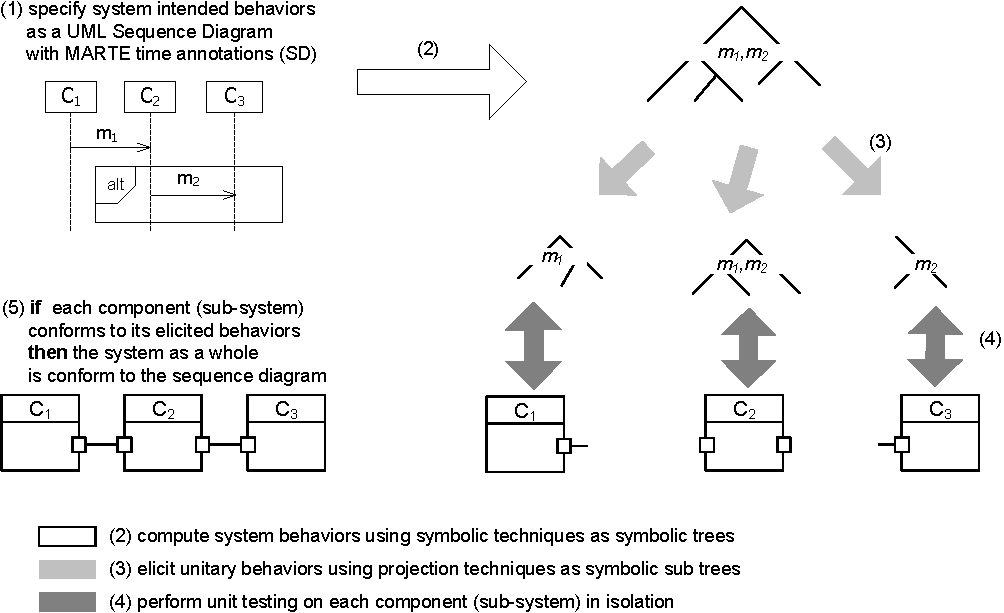
\includegraphics[scale=0.525]{approach_3.pdf}
\caption{\label{ct}Compositionnal Testing}
\end{figure}








\section{Microsoft's Verifier for Concurrent C (VCC)}

VCC is a tool from Microsoft Research
to prove correctness of annotated concurrent C programs.
It was mainly developed to verify Microsoft's \emph{Hyper-V} hypervisor.
%
It supports an own annotation language providing
e.g.\ contracts, pre- and postconditions, and type invariants.
%
It uses the Boogie tool to generate proof obligations,
and the automatic prover Z3 to prove them.
%
If an obligation is violated, the Model Viewer tool can generate a
counter-example use case.
%
VCC is available for non-commercial use from \cite{vcc}.


\section{The Proof Assistants Coq and Isabelle}


{\em Coq} is an interactive theorem prover and proof checker,
developed at INRIA, and based on
higher-order logic and the natural deduction calculus.
%
It provides the formal language {\em Gallina}, in which
mathematical definitions can be expressed as well as
executable algorithms and theorems.
%
The supporting tool for tactics-based semi-interactive development of
proofs is available from \cite{coq}.
%

{\em Isabelle}, maintained at Cambridge University,
and its predecessor {\em HOL}\footnote{
        Higher Order Logic
},
are similar tactic-oriented interactive theorem provers.
%
Isabelle is available from \cite{isabelle}.
%
While Isabelle is not yet supported in the Frama-C environment,
Coq is.


\section{The Model Checker NuSMV}

{\em SMV}\footnote{
        Symbolic Model Verifier
}
has been the first model checker based on binary decision
diagrams.
%
{\em NuSMV} is a reimplementation by the Fondazione Bruno Kessler
that is in addition capable of
performing SAT-based model-checking.
%
It supports both
Linear Temporal Logic (LTL) and Computation Tree Logic (CTL).
%
NuSMV's source code is available under an LGPL license from
\cite{nusmv}.


\section{Formal Verification of Real-Time Aspects based on Timed Automata}
\label{sct:twt:descrTA}

%\textcolor{magenta}{===== Start TWT =====}

Verifying system properties involving time is difficult with
traditional model checking methods. Commonly used \emph{temporal
  logics}, such as LTL or CTL catch discrete and qualitative aspects
of time and allow to formulate properties such as\footnote{The
  prefixes are the corresponding linear time operators.}
\begin{itemize}
  \item[\bf X] At the next point in time a property holds.
  \item[\bf F] At some future point in time a property holds.
  \item[\bf G] Always/generally (now and at any future point in time)
    a property holds. 
  \item[\bf U] A property $p$ holds until a property $q$ holds.
\end{itemize}

While it is possible to state properties that must be satisfied at
individual (discrete) points in time, continuous and quantitative
aspects of time as in the safety requirement
\begin{quote}
``The delay between receiving an emergency message and the issuing of
a brake order is less than 1 second.''
\end{quote}
are a real challenge. The problem does not stem from discrete
vs. continuous time, as any physical realisation of a real-time system
is inherently discretised by its clock. Instead, an operator for
expressing arbitrary temporal quantities or differences is
missing. Thus, for LTL and a clock of 1 kHz, it would be required to
use the operator \textbf{X} 1000 times. This notation is rather
unhandy, as it enforces to express a functional property relative to a
particular system.


This lack of expressivity is not merely a matter of notation, i.e.,
LTL or CTL, but also of the underlying semantics. Before introducing a
better suited logic we will first consider a formalism that serves as
this logic's semantics -- namely \emph{timed automata}.

\paragraph{Timed Automata}

Timed automata \cite{Alur1994} are essentially finite automata
extended with a finite set of clocks that all proceed at the same
rate. Clocks may be individually reset to zero. Clock variables can be
part of constraint expressions that may be used as transition
guards. A transition can only be taken if its guard is
fulfilled. Similarly, it is possible to specify an invariant for a
state that must be satisfied when the automaton is in this
state. Thus, we can enforce time constraints for the runs of the
automaton.

\paragraph{An Example}
The timed automaton in Figure~\ref{fig:ta:emergency1} depicts an
automaton representing an over-simplified version of an OBU subsystem
processing emergency messages. It has three states, one clock $x$ and
three actions, \textit{emg\_msg} (reception of an emergency message),
\textit{proc\_msg} (processing the message, e.g. raising an alarm) and
\textit{brake} (issueing the brake order). Upon receiving an emergency
message the clock $x$ is reset. The \textit{proc\_msg}-transition is
guarded by the clock constraint $x<1$ preventing the transition to be
taken if $x\geq 1$. The same holds for the \textit{brake}-transition.

\begin{figure}
\begin{center}
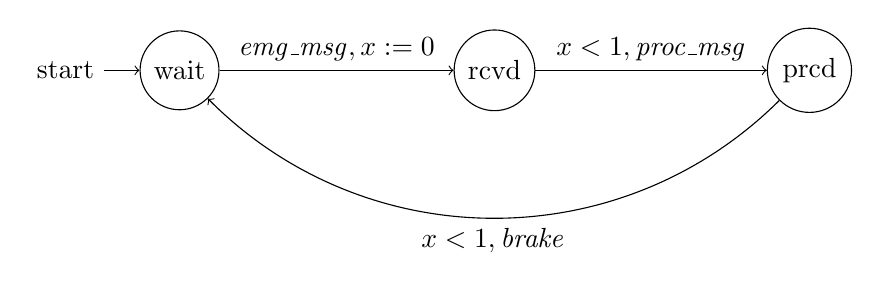
\begin{tikzpicture}[node distance=1.3cm,bend angle=45,auto]
\node [state, initial] (s1) at (0,0) { wait };
\node [state] (s2) at (4,0) { rcvd };
\node [state] (s3) at (8,0) { prcd };
\path[->] (s1) edge node {$\mathit{emg\_msg}, x:=0$}(s2);
\path[->] (s2) edge node {$x<1, \mathit{proc\_msg}$}(s3); 
\path[->] (s3) edge [bend left] node {$x<1, \mathit{brake}$}(s1);
\end{tikzpicture}
\end{center}
\caption{First (faulty) version of a timed automaton for processing
  emergency messages} 
\label{fig:ta:emergency1}
\end{figure}

One might think that the automaton from Figure~\ref{fig:ta:emergency1}
thus fulfills the safety requirement stated above. Due to the
operational semantics of timed automata this is not true: a timed
automaton in a given state can either take a transition or wait for an
arbitrary amount of time. Thus, if automaton waits in state rcvd and
$x$ exceeds one second, the system will deadlock as the next
transition is guarded by the constraint $x<1$. A run of the automaton
that could serve as counterexample is, e.g.

$$(\mathrm{wait},0)\rightarrow(\mathrm{wait},0.5)\rightarrow(\mathrm{rcvd},0.5)\rightarrow(\mathrm{rcvd},2)\rightarrow\textrm{DEADLOCK}$$

A solution to this problem is to force the automaton to proceed by
placing \emph{progress} constraints on the states. This has been done
in Figure~\ref{fig:ta:emergency2}. The transition guards have been
omitted as they are not necessary anymore. Now the safety property
``The delay between receiving an emergency message and the issuing of
a brake order is less than 1 second.'' is fulfilled.

\begin{figure}
\begin{center}
\small
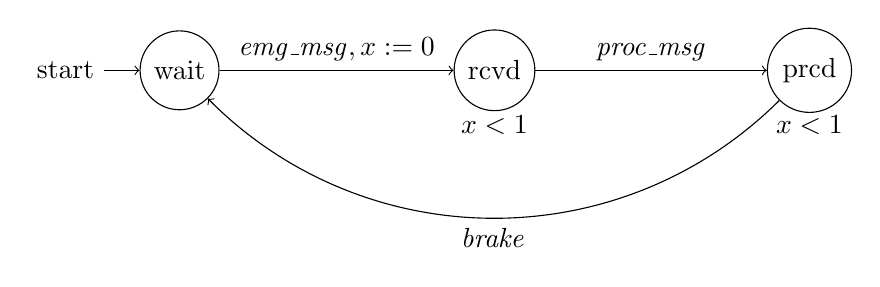
\begin{tikzpicture}[node distance=1.3cm,bend angle=45,auto]
\node [state, initial] (s1) at (0,0) { wait };
\node [state] (s2) at (4,0) { rcvd }; 
\node [state] (s3) at (8,0) { prcd };
\node at (4,-0.7) {$x<1$};
\node at (8,-0.7) {$x<1$};
\path[->] (s1) edge node {$\mathit{emg\_msg}, x:=0$}(s2);
\path[->] (s2) edge node {$\mathit{proc\_msg}$}(s3); 
\path[->] (s3) edge [bend left] node {$\mathit{brake}$}(s1);
\end{tikzpicture}
\end{center}
\caption{Corrected version of the timed automaton for processing
  emergency messages}
\label{fig:ta:emergency2}
\end{figure}

\paragraph{UPPAAL}

\textsc{Uppaal} is a tool for modelling and verifying timed automata
developed by the universities of Uppsala and Aalborg
\cite{UppaalTutorial04}. This toolkit is under constant development
and comes with an academic as well as a commercial licence. Moreover,
there is a comparably large body of literature featuring
\textsc{Uppaal}, providing introductory and industrial examples.

\textsc{Uppaal} extends timed automata with synchronisation enabling
concurrent, communicating automata representing different parts of a
system. In addition, variables other than clocks are supported making
the modelling language more powerful. The logic used for expressing
real-time properties is a subset of TCTL (Timed Computation Tree
Logic). Nesting of temporal operators is not supported leading to a
restriction in expressiveness.

\paragraph{From SysML/UML to Timed Automata}

Timed automata and statecharts in SysML/UML are both based on the
concept of finite automata. Thus, it seems reasonable to extract timed
automata from existing statecharts which is addressed in the
literature \cite{David2002, Knapp2002, Jensen2004}. In this way,
safety properties -- formalised as TCTL formulae -- can be verified in
an automated fashion for a given statechart. However, there remain
challenges:
\begin{itemize}
\item Translating hierarchical states to timed automata is not
  straight-forward and complicates matters significantly. If an
  hierarchical state-chart is flattened, structural information is
  lost and makes the timed automaton more difficult to read and
  understand. Thus, it is advisable to retain some kind of hierarchy,
  possibly by using synchronisation mechanisms.
\item Special statechart features, such as history nodes that have a
  partially undefined semantics according to the current SysML/UML
  standard \cite{fecher_29_2005}, introduce problems. As they are not
  used very often, they can possibly left out in a first iteration.
\end{itemize}

%\textcolor{magenta}{===== End TWT =====}

\chapter{Verification with Model-Based Simulation}
\label{sct:uro:systemc}

%\textcolor{magenta}{===== Start URO (first draft) =====}

This section addresses verification based on simulation. By building
an executable model of system components its real-time behaviour can
by analysed and evaluated before actually building the entire system.

\section{Modelling with SysML and SystemC}

Specifications in natural language are difficult to handle. Breaking
down an overall system description into small comprehensible parts
reduces complexity and eases interdisciplinary communication to be
more efficient in performing development tasks.

SysML, developed by the OMG (Object Management Group), is a simple but
powerful general-purpose graphical modeling language that does not
directly support executable models. However, there is a variety of
tools for code generation from UML/SysML, especially for the Eclipse
platform and the Papyrus framework that will be used in the project.

To enable model execution and especially real-time simulation it is
considered to generate semi-formal SystemC code from that abstract
SysML models. It has to be investigated whether the the SysML model
have to be adapted to a domain or language specific version. Concrete
analysis will show whether this is feasible.

SystemC is a C++ library providing an event-driven simulation
interface suitable for electronic system design at various abstraction
levels (from high level down to individual hardware components). It
enables a system designer to simulate concurrent processes. SystemC
processes can communicate in a simulated real-time environment, using
channels of different datatypes (all C++ types and user defined types
are supported). SystemC supports hardware and software synthesis (with
the corresponding tools). SystemC models are executable.

\section{Model execution and simulation}

The aim of the execution of an SystemC model is to ensure that the
working capacity (performance) of the underlying hardware system is
sufficient to meet the system requirements. It has to be analysed
which hardware resources will be needed for the OBU to avoid excessive
delays and to ensure adequate response times in critical situations.
Because of the integrated simulation enviroment, SystemC enables
scheduling analysis for average and worst-case conditions and provides
analyses of process resources for individual system functions.

In addition, by creating an executable system model from SysML or UML,
the (real time) behaviour of the system can be analysed which is not
feasible at the SysML level.

%\textcolor{magenta}{===== End URO =====}




\bibliographystyle{unsrt}
\bibliography{bibliography}
%\bibliography{Lbrr_VnV03}


%\appendix

% \chapter{Requirements on \VV}
% \label{sec:appendix}

%% \appendix

% \chapter{Requirements on \VV}
% \label{sec:appendix}


\section{Requirements on \VV from D2.9}
\label{sec:requirements-vv-D29}
%\todo{Adapt the intro text} 

The already provided requirements require a
safety plan compliant to the CENELEC EN~50126, 50128 and 50129.  This
pulls a number of requirements on V\&V, including Verification and
Validation plans. On the topic of compliance to EN~50128, one shall
also refer to the D2.2 document.


\reqfixed{02}{061}{A Verification plan shall be issued and complied
  with.}  
\subreqfixed{02}{061}{01}{The verification plan shall
  provide a method to demonstrate the requirements covering all the
  development artifacts.}  
\subreqfixed{02}{061}{02}{The verification
  plan shall state all verification activities required for each of
  these development artifacts.} 
 \reqfixed{02}{062}{A Validation Plan
  shall be issued and complied with.}  
\subreqfixed{02}{062}{01}{The
  validation plan shall provide a method to validate all functional
  and safety requirements over all development artifacts.}
\subreqfixed{02}{062}{02}{The validation plan shall state all
  validation activities required for each of these development
  artifacts.}

\reqfixed{01}{021}{The test plan shall comply the mandatory documents
  of the SUBSET-076, restricted to the scope of the OpenETCS project.}
\begin{justif}
  It will possibly be difficult to model all the tests in the course
  of the project, but the test plan should at least be complete.
\end{justif}


\reqfixed{02}{063}{Each design artifact needs a reference artifact
  which it implements (\emph{e.g.} code to detailed model, SFM to SSRS
  model\dots)} 

\subreqfixed{02}{063}{01}{The implementation between them relation
  shall be specified in detail.}  e.g.\ for state machine and a higher
level state machine mapping of interfaces, states and transition is
required.  This includes additional invariants, input assumptions and
further restrictions. This informaiton is the basis for verification
activities.

\subreqfixed{02}{063}{02}{The design of the artifacts shall be made
  such to allow verifiability as far as possible.}

\reqfixed{02}{064}{The findings from the verification shall be traced,
  and will be adequately addressed (taken into consideration, or
  postponed or discarded with a justification).}



\section{General Requirements on Verification}

\tbd{Reformulate text taken from the EN~50128 to avoid copyright infringements.}
{\footnotesize\sffamily\centering
  \begin{longtable}{||p{.15\textwidth}|p{.4\textwidth}|p{.4\textwidth}||}
    \hline\hline
    \bfseries Excerpt from EN~50128:2011 [N01] & \bfseries
    Requirement & \bfseries Project Relevance\\
    \hline\hline
    \endhead
    \hline\hline
    \endfoot
    5.3.2.7 & For each document, traceability shall be provided in
    terms of a unique reference number and a defined and documented
    relationship with other documents.  &
    fully applicable\\
    \hline 5.3.2.8 & Each term, acronym or abbreviation shall have the
    same meaning in every document.  If, for historical reasons, this
    is not possible, the different meanings shall be listed and the
    references given.  &
    \\
    \hline 5.3.2.9 & Except for documents relating to pre-existing
    software (see 7.3.4.7), each document shall be written according
    to the following rules:
    \begin{itemize}
    \item it shall contain or implement all applicable conditions and
      requirements of the preceding document with which it has a
      hierarchical relationship;
    \item it shall not contradict the preceding document.
    \end{itemize}
    &
    \\
    \hline 5.3.2.10 & Each item or concept shall be referred to by the
    same name or description in every document.  &
    \\
    \hline 6.5.4.14 & Traceability to requirements shall be an
    important consideration in the validation of a safety-related
    system and means shall be provided to allow this to be
    demonstrated throughout all phases of the lifecycle.  &
    \\
    \hline 6.5.4.15 & Within the context of this European Standard,
    and to a degree appropriate to the specified software safety
    integrity level, traceability shall particularly address
    \begin{enumerate}[a)]
    \item traceability of requirements to the design or other objects
      which fulfil them,
    \item traceability of design objects to the implementation objects
      which instantiate them.
    \item traceability of requirements and design objects to the tests
      (component, integration, overall test) and analyses that verify
      them.
    \end{enumerate}

    Traceability shall be the subject of configuration management.  &
    \\
    \hline 6.5.4.16 & In special cases, e.g. pre-existing software or
    prototyped software, traceability may be established after the
    implementation and/or documentation of the code, but prior to
    verification/validation.  In these cases, it shall be shown that
    verification/validation is as effective as it would have been with
    traceability over all phases.  & This requirement does not apply to
    the project.
    \\
    \hline 6.5.4.17 & Objects of requirements, design or
    implementation that cannot be adequately traced shall be
    demonstrated to have no bearing upon the safety or integrity of
    the system.  &
    \\
    \hline
\end{longtable}}


{\footnotesize\sffamily\centering
  \begin{longtable}{||p{.15\textwidth}|p{.8\textwidth}||}
    \hline\hline
    \textbf{Excerpt from EN~50128:2011 [N01]} & \textbf{Requirement} \\
    \hline\hline
    \endhead
    \hline\hline
    \endfoot
    6.1.4.1 & Tests performed by other parties such as the
    Requirements Manager, Designer or Implementer, if fully documented
    and complying with the following requirements, may be accepted by
    the Verifier.
    \\
    \hline 6.1.4.2 & Measurement equipment used for testing shall be
    calibrated appropriately.  Any tools, hardware or software, used
    for testing shall be shown to be suitable for the purpose.
    \\
    \hline 6.1.4.3 & Software testing shall be documented by a Test
    Specification and a Test Report, as defined in the following.
    \\
    \hline 6.2.4.2 & A Software Verification Plan shall be written,
    under the responsibility of the Verifier, on the basis of the
    necessary documentation.
    \\
    \hline 6.2.4.3 & The Software Verification Plan shall describe the
    activities to be performed to ensure proper verification and that
    particular design or other verification needs are suitably
    provided for
    \\
    \hline 6.2.4.4 & During development (and depending upon the size
    of the system) the plan may be sub-divided into a number of child
    documents and be added to, as the detailed needs of verification
    become clearer.
    \\
    \hline 6.2.4.5 & The Software Verification Plan shall document all
    the criteria, techniques and tools to be used in the verification
    process.  The Software Verification Plan shall include techniques
    and measures chosen from Table A.5, Table A.6, Table A.7 and Table
    A.8.  The selected combination shall be justified as a set
    satisfying 4.8, 4.9 and 4.10
    \\
    \hline 6.2.4.6 & The Software Verification Plan shall describe the
    activities to be performed to ensure correctness and consistency
    with respect to the input to that phase. These include reviewing,
    testing and integration.
    \\
    \hline 6.2.4.7 & In each development phase it shall be shown that
    the functional, performance and safety requirements are met.
    \\
    \hline 6.2.4.8 & The results of each verification shall be
    retained in a format defined or referenced in the Software
    Verification Plan.
    \\
    \hline 6.2.4.9 & The Software Verification Plan shall address the
    following:
    \begin{enumerate}[a)]
    \item the selection of verification strategies and techniques (to
      avoid undue complexity in the assessment of the verification and
      testing, preference shall be given to the selection of
      techniques which are in themselves readily analysable);
    \item selection of techniques from Table A.5, Table A.6, Table A.7
      and Table A.8;
    \item  the selection and documentation of verification activities;  
    \item  the evaluation of verification results gained;   
    \item  the evaluation of the safety and robustness requirements;  
    \item the roles and responsibilities of the personnel involved in
      the verification process;
    \item the degree of the functional based test coverage required to
      be achieved;
    \item the structure and content of each verification step,
      especially for the Software Requirement Verification (7.2.4.22),
      Software Architecture and Design Verification (7.3.4.41,
      7.3.4.42), Software Components Verification (7.4.4.13), Software
      Source Code Verification (7.5.4.10) and Integration Verification
      (7.6.4.13) in a way that facilitates review against the Software
      Verification Plan.
    \end{enumerate}
    \\
    \hline
\end{longtable}}

%\todo{Insert other tables.}

\section{Glossary}
\label{sec:glossary}

\begin{description}
\item[API:] Application Programming Interface. In the project, the API
  defines the interface of the EVC software to the operating system
  and hardware. \textit{The exact nature of the API still needs to be
    defined, whether it should be seen as a specification or as an
    implementation has yet to be resolved.}
\item[ATAM:] Architecture Tradeoff Analysis Method
\item [DAS2V:] Design Artifact Subject to Verification or Validation,
  e.g.\ some model or code fragment which has to be verified against
  its specification.
\item[EVC:] European Vital Computer
\item[FLOSS:] Free/Libre/Open Source Software
\item[FFM:] Fully Formal Model. Sometimes called ``Strictly Formal
  Model''.  A model of a part of the design which has a fully formal
  semantics and can thus be subjeced to rigorous analysis methods from
  the domain of mathematical or computational logic.
\item[HW:] Hardware
\item[SAAM:] Software Architecture Analysis Method 
\item[SFM:] Semi Formal Model. A model of some part of the design
  whose semantical interpretation is either not fully fixed or is
  similar to that of a program. I.e., the interpretation might depend
  on variations in the code generation or compilation, or it does not
  resolve ``semantic variation points'' (UML).
\item[SW:] Software
\end{description}





\nocite{*}
%===================================================
%Do NOT change anything below this line

\end{document}
